%-----------------------------------------------------------------------
%
% File Name: thesis.tex
%
% Author: Kelley, D. B.
%
% Revision: $Id$
%
%-----------------------------------------------------------------------

% document class and packages
\documentclass[12pt,notitlepage]{report}
\usepackage{bibunits}
\usepackage{suthesis}
\usepackage{graphicx}
\usepackage{color}
\usepackage{amsmath}
\usepackage{amssymb}
\usepackage{amsfonts}
\usepackage[bookmarksnumbered, bookmarksopen, breaklinks, colorlinks, linkcolor=blue, citecolor=magenta]{hyperref}

%\usepackage{caption}
%\usepackage{rotating}
%\usepackage{tensor}

\pdfoutput=1
\DeclareGraphicsExtensions{.pdf,.png}

\hbadness=10000

% new command definitions
\newcommand{\half}{\frac{1}{2}}
\newcommand{\ospsd}{\ensuremath{S_n\left(\left|f_{k}\right|\right)}}

% journal definitions
\newcommand{\apj}{{\it Astrophysical J.}}
\newcommand{\apjl}{{\it Astrophysical J.}}
\newcommand{\aap}{{\it Astron. and Astrophys.}}
\newcommand{\cmp}{{\it Commun. Math. Phys.}}
\newcommand{\grg}{{\it Gen. Rel. Grav.}}
\newcommand{\cqg}{{\it Class. Quant. Grav.}}
\newcommand{\lr}{{\it Living Reviews in Relativity}}
\newcommand{\mnras}{{\it Mon. Not. Roy. Astr. Soc.}}
\newcommand{\pr}{{\it Phys. Rev.}}
\newcommand{\prl}{{\it Phys. Rev. Lett.}}
\newcommand{\prd}{{\it Phys. Rev. D}}
\newcommand{\pra}{{\it Phys. Rev. A}}
\newcommand{\prsl}{{\it Proc. R. Soc. Lond. A}}
\newcommand{\ptrsl}{{\it Phil. Trans. Roy. Soc. London}}
\newcommand{\rmp}{{\it Rev. Mod. Phys.}}

\newcommand{\tcr}{\textcolor{red}}
\newcommand{\tcb}{\textcolor{blue}}
\newcommand{\tcm}{\textcolor{magenta}}
\newcommand{\tcg}{\textcolor{green}}
\newcommand{\tcp}{\textcolor{purple}}

\begin{document}
\title{Angular trapping of a mirror using radiation pressure}
\author{David B. Kelley}
\majorprof{Stefan Ballmer}
% For the following line, if you got a masters, list it first. Otherwise, leave the first of the two entries blank, like the line below it.
\previousdegree{M.S. Syracuse University, Syracuse, NY, 2013}{B.S. Massachusetts Institute of Technology, Cambridge, MA, 2010}
%\previousdegree{}{B.S. Massachusetts Institute of Technology, Cambridge, MA, 2010}
\submitdate{October 2015}
\degree{Doctor of Philosophy}
\program{Physics}
\copyrightyear{2015}
\majordept{Physics}
\havededicationtrue
\dedication{to\\ my parents and Emma}
\haveminorfalse
\copyrighttrue
\doctoratetrue
\figurespagetrue
\tablespagetrue

\Abstract{% taken from angular theory paper
Alignment control in gravitational-wave detectors has consistently proven to be a difficult problem due to the stringent noise contamination requirement for the gravitational wave readout and the radiation-pressure induced angular instability in Fabry-Perot cavities (Sidles-Sigg instability \cite{Sidles06}).
I present the development, implementation, and measurement of a dual-carrier control scheme which uses radiation pressure to control a suspended mirror,
trapping it in the longitudinal degree of freedom and one angular degree of freedom. 
}
\beforepreface
\prefacesection{Preface}
The work presented in this thesis stems from my participation in the LIGO
Scientific Collaboration (LSC). This work does not reflect the
scientific opinion of the LSC and it was not reviewed by the collaboration.

\vspace*{0.5cm}
\noindent The theory of optical trapping in two degrees of freedom in chapter \ref{ch:introduction} is based on

\vspace*{0.25cm}

\noindent A.~Perreca~{\it et~al.}, ``Multi-dimensional optical trapping of a mirror,''
\prd~{\bf 89} (2014) 122002.

%\vspace*{0.5cm}
%
%\noindent Chapter \ref{ch:photothermal} is based on material from
%
%\vspace*{0.25cm}
%
%\noindent David B. Kelley~{\it et~al.}, ``Observation of photo-thermal feed-back in a stable dual-carrier optical spring,''  to be submitted to
%\prd.
%
%\vspace*{0.25cm}
%
%\noindent Chapter \ref{ch:angular} is based on 
%
%\vspace*{0.25cm}
%
%\noindent David B. Kelley~{\it et~al.}, ``Angular Trap Demonstration,'' to be submitted to
%\prd

\prefacesection{Acknowledgments}
I would like to thank many people for all the wonderful things they have done over the past 3000 years or so.



\afterpreface

\Chapter{Introduction}
\label{ch:introduction}
% $Id$

In chapter \ref{c:findchirp} we describe in detail the algorithms used to
inspiral signals from binary neutron starts and binary black hole MACHOs in
the LIGO data.  findchirp. We first carefully define the conventions that we
use for analysis quantities in section \ref{s:conventions}; in particular the
definition of the Fourier transform and the power spectral density. Section
\ref{s:waveforms} gives a brief description of the the waveforms used and
section \ref{s:matchedfilter} describes the implementation of the matched
filter.  Spurious noise may cause the output of the matched filter to be large
and so in section \ref{s:chisq} we describe our implementation of the $\chi^2$
time--frequency discriminator proposed in~\cite{allen}. Section
\ref{s:practical} contains additional details of the search particular to our
implementation: the computation of the inverse power spectrum and the trigger
selection algorithm. This is followed by a brief conclusion which summarized
the methods used and outlines some future directions for improvement.

\section{Fourier Transform Conventions}
\label{s:ftconv}

There are two possible sign conventions for the Fourier transform of a time
domain quantity $v(t)$. In this thesis, we define the Fourier transform
$\tilde{v}(f)$ of a $v(t)$ to be
\begin{equation}
\label{eq:ft}
\tilde{v}(f)=\int_{-\infty}^\infty dt\,v(t)\, e^{- 2 \pi i f t}
\end{equation}
and the inverse Fourier transform to be 
\begin{equation}
\label{eq:ift}
v(t)=\int_{-\infty}^\infty df\,\tilde{v}(f)\, e^{2 \pi i f t}.
\end{equation}
This convention differs from that used in some gravitational wave literature,
but is the adopted convention in the LIGO Scientific Collaboration.

%\Chapter{Suspensions}
%\label{ch:suspensions}
%Suspending the optics is one of the most complicated parts of the experiment.
The optics are constructed as discs with roughly 76 mm (3 inch) diameters. 
They are suspended from modified Small Optics Suspensions (SOSs) and controlled with Optical Sensing Electro-Magnets (OSEMs).

\section{Input coupler}

The input coupler (see fig \ref{fig:inputcoupler}) is designed to hold three mirrors at specific positions and angles. The mirrors are 0.5 inches in diameter with 7.5 cm RoC. They are mounted in an approximately 300 gram aluminum disk.
The central mirror forms the straight cavity with the end mirror, while the two mirrors on the side are part of the folded cavity. 
The angle and, to a lesser degree, z position of the two side mirrors are adjustable using set screws. 
 
For each of the adjustable mirrors, set screws push on the bevel of the back surface of the mirror. 
The mirror is held in place by a Teflon tube placed on the front side of the mirror, which is in turn clamped down with springs on screws.
This gives us the flexibility to adjust for manufacturing defects and to adjust the beam separation on the end mirror after construction.

Tapped screws in the top and bottom allow for precision correction of the center of mass of the mass after suspension.
The mirrors are shifted laterally to make the mirrors fit inside the 3.0 inch diameter of the aluminum mass.

The design concerns governing the placement of the holes include the separation of the beams, the angle of the folded cavity, and the desired lengths of the two cavities. 

\begin{figure}[hp]
	\centering
		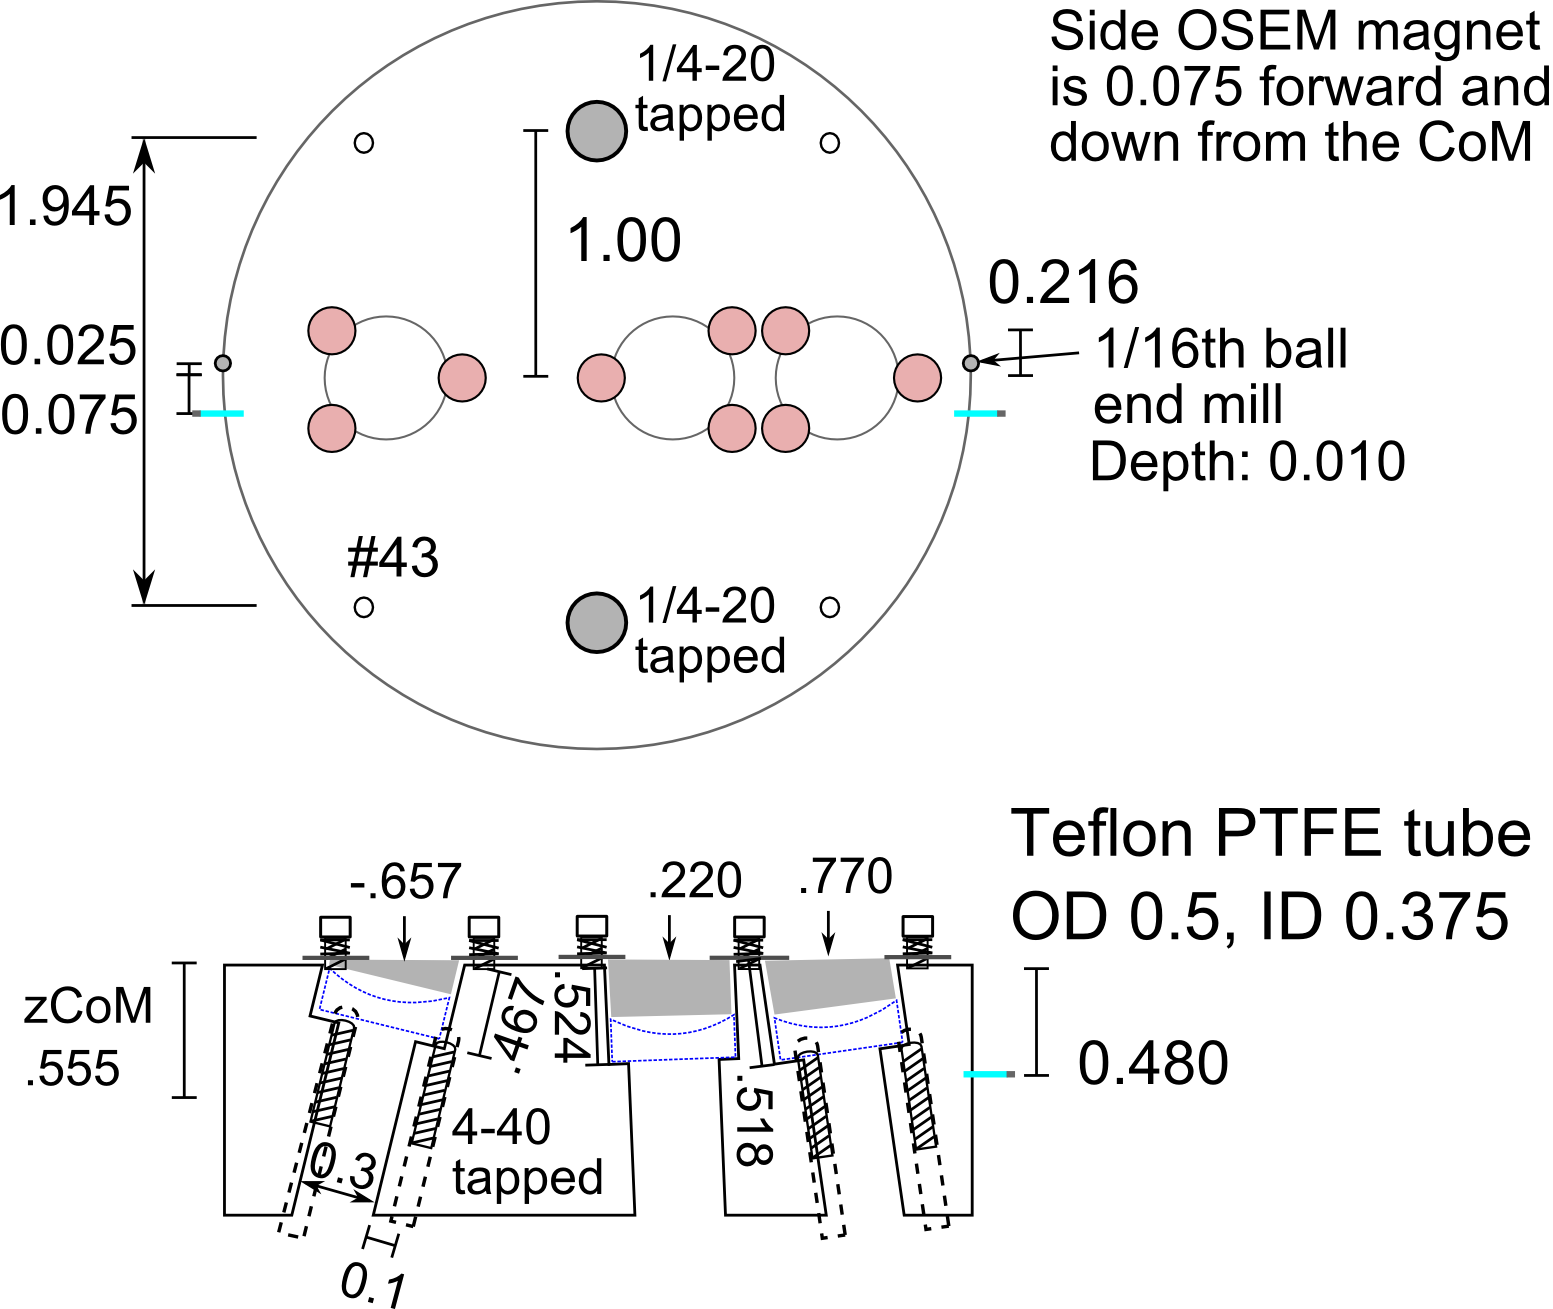
\includegraphics[width=.9\textwidth]{figures/suspensions/inputcoupler.png}
	\caption[Input coupler]{The input coupler for the cavity. Three 0.5 inch diameter mirrors with 7.5 cm RoC are held at specific angles inside an aluminum disk. The two side mirrors are adjustable using set screws, while the central mirror is fixed.}
	\label{fig:inputcoupler}
\end{figure}
 
\section{End mirror}

The end mirror has a diameter of 0.305 inches, a radius of curvature of 5 cm, and a mass of 0.4 grams. It is suspended by glass fibers from a steel ring, which is in turned suspended from a modified SOS. The suspension is pictured in \ref{fig:smallmirrorpic}.

The fibers are manufactured by cold welding a fused silica rod onto a mirror blank, creating a nub, then pulling a fiber off it, to a length of about 1 inch. Once the fiber cools, we break the cold weld. This leaves us with a nub attached to a fiber, which is in turn attached to a silica rod. The silica rod is glued into an aluminum block, which is screwed down to the steel ring. The nubs are then glued to the actual mirror using Optocast 3553. Because the nubs were created on a mirror blank with the same diameter, the volume of glue required is minimized, reducing the thermal noise effects of the glue joint. After gluing on all three fibers, the fibers are tensioned to raise the resonance of the position mode to the desired frequency.

\begin{figure}[htbp]
	\centering
		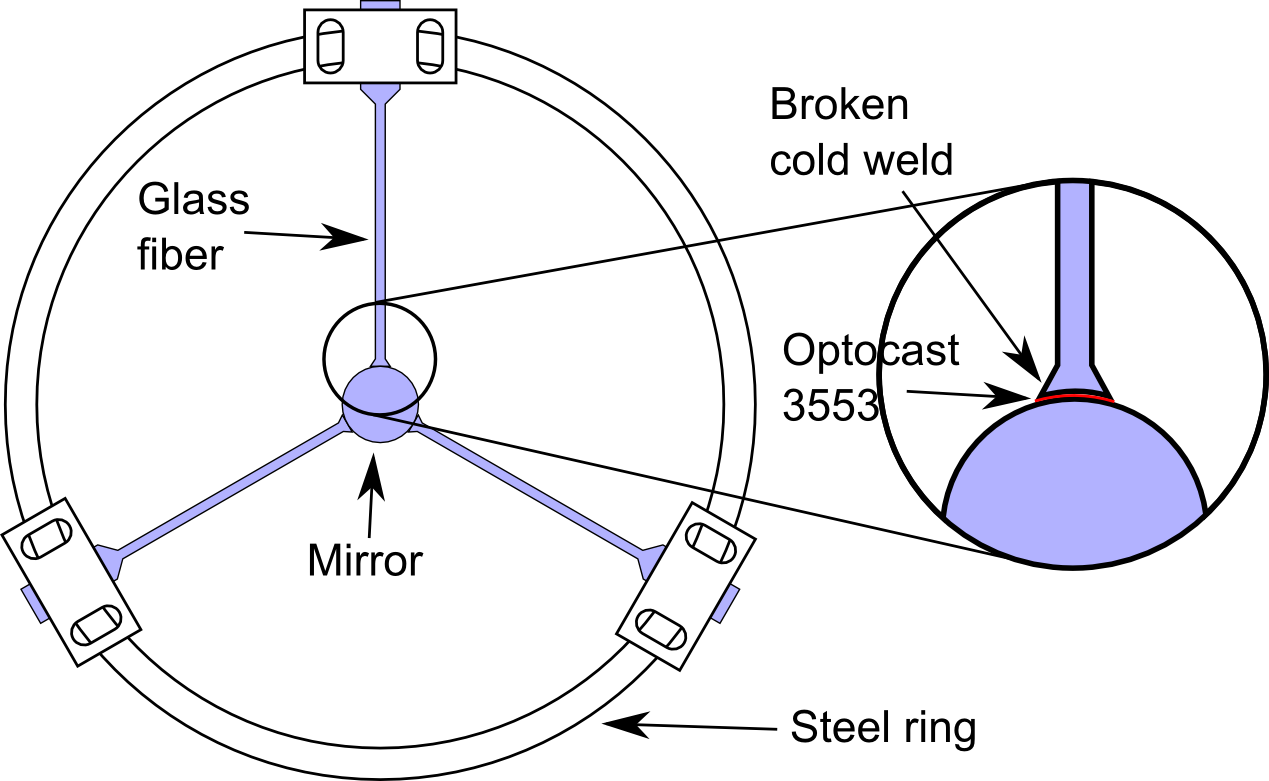
\includegraphics[width=.9\textwidth]{figures/suspensions/smallmass2.png}
	\caption[End mass suspension]{End mass suspension. A 0.4 gram mirror is suspended from a steel ring using glass fibers.}
	\label{fig:smallmassdiagram}
\end{figure}




\section{Blade Springs}
%This is a partial procedure that we have adopted to design a vertical isolation system for a large platform
%used to host the Small Optic Suspensions (SOS) that support our Trap-Cavity. The platform is an aluminum disk with two SOS structures and counterweights, totaling 75 Kg, which will
%be suspended with 3 wires, each attached to a blade spring in order to increase vertical isolation. Fig.\ref{fig:topplate} shows the top plate with its blade springs. The clamp bases will be cut out in order to make them fit on to the plate. 

%\begin{figure}[ht]		
%\centering
%\includegraphics[width=7cm]{topplate.png}
	%\caption{\emph{View of the top plate from below.}}
	%\label{fig:topplate}
%\end{figure}

%We want a relatively low bounce mode frequency, less than 1Hz, with a minimized coupling
%of the vertical motion into the longitudinal one. This requires adjusting dimensional parameters in order to keep the stress under the allowed limit of the material that we are going to use.
This is a discussion of the relevant physics to the construction of blade spring suspensions for a small optics suspension.

This theoretical parts of the paper are based primarily on the notes posted in the DCC
\footnote{https://dcc.ligo.org/LIGO-T030285}.

\subsection{A little theory}
\label{sec:theory}

\begin{figure}[ht]		
\centering
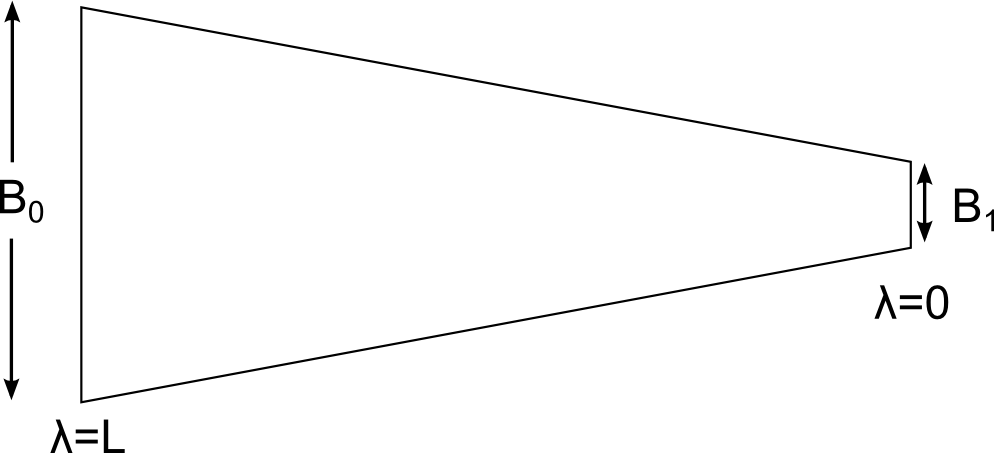
\includegraphics[width=7cm]{figures/suspensions/bladeWidth.png}
	\caption[Blade springs]{Profile drawing of a deflected blade spring. R is the radius of the circle described by the blade spring
	when it is under stress. L is the length of the blade, $b_0$ is the large base and $b_1$ is the small base. $\lambda$ is the distance along the blade}
	\label{fig:bladeIllustration}
\end{figure}

The paper gives the general formula for an elastic beam under a load (see Rourke's formulas for stress and strain, eq. 8.1-4):

\begin{eqnarray}
\frac{E}{R(\lambda)} = \frac{M(\lambda)}{I(\lambda)}
\label{eq:R}
\end{eqnarray}
 
Here $\lambda$ is the distance along the blade (with the $\lambda=0$ at the tip), $E$ is the Young's modulus, $R$ is the radius of curvature at $\lambda$, $I$ is the area moment of inertia at $\lambda$, and $M$ is the bending moment at $\lambda$, expressed as: 

\begin{eqnarray}
M = m g \lambda
\label{eq:M}
\end{eqnarray}

where m is mass supported, g is $9.81 \mbox{m/s}^2$.

$b = b_1+(b_0-b_1) \frac{\lambda}{L}$ is the width between $\lambda=0$ ($b=b_1$) and $\lambda=L$ ($b=b_0$) (see figure \ref{fig:bladeIllustration}) so

\begin{eqnarray}
I = \frac{b t^3}{12} = (b_0-b_1)\frac{t^3}{12} \frac{\lambda}{L}+b_1\frac{t^3}{12}
\label{eq:I1}
\end{eqnarray}


where $t$ is the thickness of the blade and $L$ is the blade length.  If we consider the blade to be triangular ( $b_1=0$), $I$ becomes

\begin{eqnarray}
I = \frac{b_0t^3}{12} \frac{\lambda}{L}
\label{eq:Itri}
\end{eqnarray}

Then we see that 

\begin{eqnarray}
\frac{E}{R(\lambda)} = \frac{M(\lambda)}{I(\lambda)} = 
\frac{m g \lambda}{b_0\frac{t^3}{12} \frac{\lambda}{L}} = 
\frac{12 m g L}{b_0 t^3} \quad \rightarrow \quad R=constant
\label{eq:E/R}
\end{eqnarray}

In other words, R is constant along the blade (the blade profile is circular). We can accomplish this behavior by specifying that the wire is clamped where the end of the `triangle' should be.

%You may have noticed that the calculation is based on an initially flat beam. 
%We attempted to add a cosine term to account for the monting angle, but the predictions were inaccurate.

% However, the modification to the moment calculation for a beam deflection $\theta$ is as simple as accounting for the change in deflection force ($m g \rightarrow m g  \mbox{cos}(\theta)$) (this is assuming that the blade is not compressable in the $\lambda$ direction).

Thus we can, without difficulty, treat a change in force on the spring (for instance by changing the mass) as a change in the radius of curvature of the blade.

%This prediction will obviously break if the end of the spring goes more than one radius below the highest point.

From eq.\ref{eq:E/R} we obtain $R$

\begin{eqnarray}
R(\lambda) = R = \frac{E b_0 t^3}{12 m g L}
%R(\lambda) = R = \frac{E b_0 t^3}{12 m g L \mbox{cos}(\theta)}
\label{eq:Rend}
\end{eqnarray}

From eq.{\ref{eq:Rend}} we can obtain the bounce mode frequency $f_b$

\begin{eqnarray}
f_b = \frac{1}{2\pi}\sqrt{\frac{E b_0 t^3}{6 m L^3}}
%f_b = \frac{1}{2\pi}\sqrt{\frac{E b_0 t^3}{6 m L^3 \mbox{cos}(\theta)}}
\label{eq:fb}
\end{eqnarray}

and the maximum stress in the blade as:

\begin{eqnarray}
\sigma = \frac{6 m g L}{ b_0 t^2};
%\sigma = \frac{6 m g \mbox{cos}(\theta)L}{ b_0 t^2};
\label{eq:stress}
\end{eqnarray}

We can use equation \ref{eq:stress}, solved for $b_0$, to simplify equation \ref{eq:fb}, thus

\begin{eqnarray}
f_b = \frac{1}{2\pi}\sqrt{\frac{E g t}{L^2 \sigma}}
\label{eq:fb2}
\end{eqnarray}

Given a target stress $\sigma$, a target bounce frequency $f_b$, and a length limit $L$ based on the chamber dimensions, we can determine the proper thickness $t$ for the blade.

If we manipulate equations \ref{eq:fb2} and \ref{eq:stress}, we get

\begin{eqnarray}
t = \frac{(2 pi f_b L)^2 \sigma}{E g} = \sqrt{\frac{6 m g L}{ b_0 \sigma}}
%t = \frac{(2 pi f_b L)^2 \sigma}{E g} = \sqrt{\frac{6 m g \mbox{cos}(\theta)L}{ b_0 \sigma}}
\label{eq:thickness}
\end{eqnarray}

This equation gives the minimum requirement to make a blade spring.

% We are left with two related parameters, $\theta$ and $b_0$ which can be written as follow from eq:\ref{eq:stress} eq.\ref{eq:thickness}:  
% 
% \begin{eqnarray}
% \frac{b0}{cos\Theta}=\frac{6mgL}{\sigma t^2}
% \label{eq:b0cos}
% \end{eqnarray}
% 
% We must adjust both, maintaining the constant thickness, to minimize the coupling of vertical motion to horizontal motion at the tip of the blade.  To do this, we plot the blade profile with small variations to the supported mass, simulating a vertical force, and find the mounting angle with the minimum horizontal fluctuation (effective length $z_{max}$ fluctuation) for the supported mass:
% % (See figures \ref{fig:massvlen}):

%\begin{figure}[ht]		
%\centering
%\includegraphics[width=400pt]{massvlen.png}
	%\caption{\emph{Effective blade length as a function of mass applied. By recalculating the radius of curvature with varying masses, we can simulate the effect of applying a vertical force to the payload. }}
	%\label{fig:massvlen}
%\end{figure}


% \subsection{Blade profile plot}
% %$f_b$ is the predicted bounce mode frequency for the blade spring, loaded with 25 kg.
% 
% We can plot the blade profile by changing to a basis $\phi = \frac{\lambda}{R}+\phi_i$ where $\phi_i = \pi/2 -\theta$ is the initial $\phi$ such that the initial blade spring angle is $\theta$, then we can do a parametric plot (see Fig. \ref{fig:bladeIllustration}) with the longitudinal axes $z$ and the vertical axes $y$ defined as following:
% 
% \begin{eqnarray}
% z&=&-R(\mbox{cos}(\phi)-\mbox{cos}(\phi_i))\\
% y &=& R(\mbox{sin}(\phi)-\mbox{sin}(\phi_i))
% \label{eq:yzparam}
% \end{eqnarray}
% 
% Using this method, we can easily predict important blade measurements such as effective length, maximum blade height, and tip height.
%  %$z=-R(\mbox{cos}(\phi)-\mbox{cos}(\phi_i))$ and $y = R(\mbox{sin}(\phi)-\mbox{sin}(\phi_i))$ as (See Fig.\ref{fig:bladeIllustration}) . 
%We can now look at the blade spring profile when different weights are attached to it. We notice from Fig.\ref{fig:bladeprofilen} the changes in height at different applied forces and at a fixed initial angle. \tcb{is this plot correct?}

%\tcb{From this plot, we can determine the maximum height, the effective length, and the lateral change in the tip due to vertical force fluctuations.}

%\begin{figure}[ht]
	%\centering
		%\includegraphics[width=300pt]{bladeprofile.png}
	%\caption{\emph{Blade profile for $\theta = 49^\circ$.}}
	%\label{fig:bladeprofile}
%\end{figure}

 
% and \ref{fig:heightvlen}.
%
%At the peak of the curves, you can see that for small variations in mass, the slope goes to zero.
%
%%%%%%  MATERIALS  %%%%%%%%%%%%%%%%%%%%%%%%%%%%%%%%%%%%%%%%%%%%%%%%%%
\subsection{Materials}

The LIGO-recommended material is ``maraging'' steel (sometimes known by the tradename Vascomax), which is easy to machine, but becomes incredibly hard when baked.  One drawback of this material is that it can corrode over time.  To combat this, LIGO recommends putting a nickel plating on the blades \footnote{https://dcc.ligo.org/LIGO-E0900023}.  The hardness of the final product is the primary reason it is used.  This material is difficult and expensive (best offer was \$1200 for six blade's worth) to buy in small quantities.  

As an alternative, we are considering ``full hardened'' 301 stainless steel.  It is a factor of about 2.5 weaker than the maraging steel, but we have have found that workable solutions exist.

A third alternative is 17-4 precipitation hardened (PH) stainless.  This material is similar to maraging steel in that it becomes harder when you bake it.  Baking at 900 F for one hour results in a yield strength of 200000 psi = 1379 MPa.  Baking longer or at a higher temperature makes the material a bit sorfter, but this behavior is understood and fairly error-tolerant \footnote{http://www.aksteel.com/pdf/markets\_products/stainless/precipitation/17-4\_PH\_Data\_Bulletin.pdf}

One more alternative which LIGO uses for the small blade springs is 304 stainless (yield strength of 200 MPa) because the expected strain in the small blades is about 80 MPa.

For comparison, McMaster has details of many of the metals that are available \footnote{http://www.mcmaster.com/library/20121105/8984KAC.pdf}. All of the metals we are considering are on the LIGO vacuum compatible materials list\footnote{https://dcc.ligo.org/LIGO-E960050}.

When we are determining the maximum amount of stress that the blade can withstand before deforming, we typically use the yield strength.  This is the amount of stress that causes the metal to deform by 0.2\%.  We have chosen as a target strain 60\% of the yield strength.

One LIGO document \footnote{https://dcc.ligo.org/LIGO-T0900324} adds a factor related to the Poisson's Ratio to the Young's Modulus which effectively increases the strain.  This is attributed to a change in the strain of the material due to bending.  Our predictions seem to work better with this factor removed, but we have chosen to keep the factor for the moment because it represents the `worst case' scenerio.  



\begin{table}[ht]
	\centering
		\begin{tabular}{ l | l | l | l | l }
			Steel & E (GPa) & E (psi) & $\sigma_{max}$ (MPa)  & $\sigma_{max}$ (PSI) \\ \hline
			C350 Maraging & 200 & $29\times10^6$ & 2344 & $34\times10^4$ \\ \hline
			301 Stainless & 193 & $28\times10^6$ & 965 & $14\times10^4$ \\ \hline
			17-4 PH Stainless & 196.5 & $28.5\times10^6$ & 1379 & $20\times10^4$\\ \hline
			304 Stainless &  193 & $28\times10^6$ & 207 & $3\times10^4$
		\end{tabular}
	\caption{Characteristics of proposed materials.}
	\label{tab:materials}
\end{table}

\subsection{Blade spring design}

Criteria for the design following the section \ref{sec:theory}:

\begin{enumerate}
	\item Maintain safe levels $\leq 80\%$ of material stress limits:
	$\sigma\leq0.8\sigma_{max}$.
	\item Blades must be mounted on top of the existing suspensions; smaller is better. 
%  \item All parts must fit within the area of the 27 inch diameter top plate in the bell jar. The length $L$ of the blade springs is fixed at 19''; when under load the bending will reduce the effective length.
  \item Choose a `small' (within reason) bounce mode frequency (This determines $t$). 
  % \item Choose a `small' (within reason) bounce mode frequency (from here we get $t$). 
	\item Minimize vertical to horizontal coupling, looking at the effective length $z_{max}$ as a function of different loads and angles. We could adjust the weight for a given angle or at fixed weight we adjust the angle. The latter is our way to go.
	
\end{enumerate}
%Using equations from \ref{eq:Rend} to \ref{eq:thickness} we have found parameters that satisfy the criteria.  We are using 17-4 stainless steel.  
%The maximum stress of this design is only 60\% of the expected yield strength of the material.  
%This gives us more leeway with the construction and reduces the chance of failure sue to improper baking.  
%The final design schematic is shown in figure \ref{fig:bladeschematic}

%We have two possibilities, one more aggressive in pursuing the lowest bounce mode frequency than the other.  Both utilise 301 stainless steel.

%\subsection*{Proposal 1: $f_b$= 0.9 Hz}
%
%\begin{table}[ht]
%\centering
%\begin{tabular}{ l | l | l }
%\bf{Parameter}& \bf{Metric} & \bf{Imperial} \\ \hline
%Blade length, $L$ & 48.3 cm & 19.0 in \\ \hline
%Blade base width, $b_0$ & 7.9 cm & 3.13 in \\ \hline
%Blade thickness, $t$ & 2.76 mm & 1088 in \\ \hline
%Mounting angle, $\theta$ & 0.850 rad & $48.69^\circ$ \\ \hline
%Supported mass, $m$ & 25 kg & 55 lbs
%\end{tabular}
%\caption{Proposed blade parameters}
%\label{tab:params09}
%\end{table}
%
%\begin{table}[ht]
%\centering
%\begin{tabular}{ l | l | l}
%\bf{Result} & \bf{Metric} & \bf{Imperial} \\ \hline
%Bounce Frequency, $f_b$ & 0.9 Hz \\ \hline
%Max height & 12.9 cm & 5.08 in \\ \hline
%Tip height & 9.6 cm & 3.78 in \\ \hline
%Effective length & 44.0 cm & 17.34 \\ \hline
%Maximum Stress, $\sigma$ & 772 MPa & 112000 PSI
%\end{tabular}
%\caption{Characteristics of proposed blade design}
%\label{tab:results09}
%\end{table}
%\subsection*{Proposal 2: $f_b$= 0.8 Hz}
%
%\begin{table}[H]
%\centering
%\begin{tabular}{ l | l | l }
%\bf{Parameter} & \bf{Metric} & \bf{Imperial} \\ \hline
%Blade length, $L$ & 48.3 cm & 19.0 in \\ \hline
%Blade base width, $b_0$ & 9.1 cm & 3.59 in \\ \hline
%Blade thickness, $t$ & 2.18 mm & 0.0860 in \\ \hline
%Mounting angle, $\theta$ & 1.078 rad & $61.75^\circ$ \\ \hline
%Supported mass, $m$ & 25 kg & 55 lbs
%\end{tabular}
%\caption{Proposed blade parameters}
%\label{tab:params08}
%\end{table}
%
%\begin{table}[H]
%\centering
%\begin{tabular}{ l | l | l}
%\bf{Result} & \bf{Metric} & \bf{Imperial} \\ \hline
%Bounce Frequency, $f_b$ & 0.8 Hz \\ \hline
%Max height & 15.8 cm & 6.22 in \\ \hline
%Tip height & 11.7 cm & 4.59 in \\ \hline
%Effective length & 41.6 cm & 16.38 \\ \hline
%Maximum Stress, $\sigma$ & 772 MPa & 112000 PSI
%\end{tabular}
%\caption{Characteristics of proposed blade design}
%\label{tab:results08}
%\end{table}
%\newpage
%\subsection*{Proposal: Large Springs $f_b$= 0.9 Hz}
%
%\begin{table}[ht]
%\centering
%\begin{tabular}{ l | l | l }
%\bf{Parameter}& \bf{Metric} & \bf{Imperial} \\ \hline
%Blade length, $L$ & 48.3 cm & 19.0 in \\ \hline
%Blade base width, $b_0$ & 7.8 cm & 3.07 in \\ \hline
%Blade thickness, $t$ & 2.76 mm & 1088 in \\ \hline
%Mounting angle, $\theta$ & 0.849 rad & $48.67^\circ$ \\ \hline
%Supported mass, $m$ & 25 kg & 55 lbs\\\\
%\bf{Result} & \bf{Metric} & \bf{Imperial} \\ \hline
%Bounce Frequency, $f_b$ & 0.9 Hz \\ \hline
%Max height & 12.9 cm & 5.08 in \\ \hline
%Tip height & 9.6 cm & 3.77 in \\ \hline
%Effective length & 44.0 cm & 17.34 \\ \hline
%Maximum Stress, $\sigma$ & 786 MPa & 114000 PSI
%\end{tabular}
%\caption{Characteristics of proposed blade design}
%\label{tab:results09}
%\end{table}


%\subsection*{Proposal 2: $f_b$= 0.8 Hz}


%There are distinct advantages for each proposal.  The higher maximum blade height of the 0.8 Hz blade will result in a longer pedestal for the clamp (to lower the mounting point), lowering the resonances of the pedestal (but we expect they will still be very high).  The shorter effective length of the 0.8 Hz blade will make our setup a bit more flexible.  The larger radius of curvature of the 0.9 Hz blade will reduce the horizontal-vertical coupling. 
%
%The mounting angle may or may not be an issue, depending on how well our simulations work.  The frequency difference actually makes very little difference for anything over 5 Hz.

%\newpage



%
%\subsection{Couplings}
%
%With a vertical seismic noise RMS motion of $10^{-7}$ m, we could expect that to be coupled to the `twist' mode of the optical table (because the springs all point in the same direction around the center of the table).
%
%If properly aligned (parameters properly chosen), we are in a situation where there is a minimised coupling between the vertical and the longitudinal motion. The horizontal motion is described by $z$ and the vertical motion is described by the tip motion along $y$ (see Fig.\ref{fig:heightvlen}).
%%
%%\begin{figure}[htp]		
%%\centering
%%\includegraphics[width=350pt]{heightvlen.png}
	%%\caption{\emph{Effective blade length as a function of blade tip height. A vertical motion of $1\,$mm longitudinal motion coupling
	%%of the order of a micron.}}
	%%\label{fig:heightvlen}
%%\end{figure}
%
%
%We could expect couplings of up to $4\times10^-3$ if we are off from that point by a milimeter.  Thus a vertical RMS displacement of $10^{-7}$ m could result in a twist RMS displacement of $10^{-10}$ m.  
%Fig.\ref{fig:seismic} shows seismic motion coupled into vertical and longitudinal motions. 
%
%%\begin{figure}[hp]
	%%\centering
		%%\includegraphics[width=400pt]{seisplot.png}
	%%\caption{\emph{Expected seismic motion, taken from David's noise budget. At this level the horizontal coupling (red line)  does not seem to be an issue. }
%%}
	%%\label{fig:seismic}
%%\end{figure}
%
%
%%\begin{figure}[p]
	%%\centering
		%%\includegraphics[width=600pt, angle=90]{blade.png}
	%%\caption{\emph{Design of large blade}}
	%%\label{fig:bladeschematic}
%%\end{figure}
%
%\newpage

\subsection{Small blade}

At the same time, we are designing a similar suspension to be mounted on top of each SOS.  These will be much smaller, but will follow the same design principles.


For the small spring system, our design is very similar to the parameters used in the HAM AUX design for ALIGO \footnote{https://dcc.ligo.org/LIGO-T1000339}  We can use 304 Stainless or 17-4 Stainless with little impact on the final performance.  The maximum stress of this design is only 40\% of the expected yield strength of 304 and much less than that for 17-4.  This gives us more leeway with the construction and reduces the chance of failure due to improper baking.  The final design schematic is shown in figure \ref{fig:babyschematic}.  For the small design we have chosen to neglect the Poisson Ratio factor because the bending is much smaller.  We are motivated to do this by the HAM AUX design mentioned earlier.

\begin{table}[ht]
\centering
\begin{tabular}{ l | l | l }
\bf{Parameter}& \bf{Metric} & \bf{Imperial} \\ \hline
Blade length, $L$ & 7.68 cm & 3.0 in \\ \hline
Blade base width, $b_0$ & 3.3 cm & 1.3 in \\ \hline
Blade thickness, $t$ & 0.51 mm & 0.020 in \\ \hline
Mounting angle, $\theta$ & 0.083 rad & $4.78^\circ$ \\ \hline
Supported mass, $m$ & 0.15 kg & 0.33 lbs\\\\
\bf{Result} & \bf{Metric} & \bf{Imperial} \\ \hline
Bounce Frequency, $f_b$ & 7.19 Hz \\ \hline
Max height & 2 mm & 0.08 in \\ \hline
Tip height & 2 mm & 0.06 in \\ \hline
Effective length & 7.7 cm & 3.0 in \\ \hline
Maximum Stress, $\sigma$ & 81 MPa & 11700 PSI
\end{tabular}
\caption{Characteristics of proposed blade design}
\label{tab:resultsBaby}
\end{table}

\subsection{Coupling}
For the small spring system, we do not need to worry about this coupling because the motion will not couple to the position degree of freedom to first order.  We should note that changing the effective length would result in a change in the yaw mode resonance of the suspended structure, which may be an issue. 



\begin{figure}[hp]
	\centering
		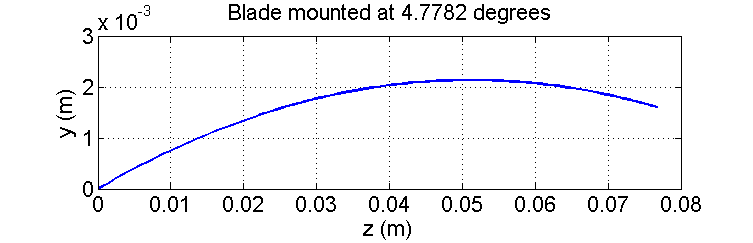
\includegraphics[width=.9\textwidth]{figures/suspensions/babybladeprofile.png}
	\caption[Blade profile for small suspension.]{Expected profile of the small blade supporting 300 grams.}
	\label{fig:babybladeprofile}
\end{figure}





\begin{figure}[p]
	\centering
		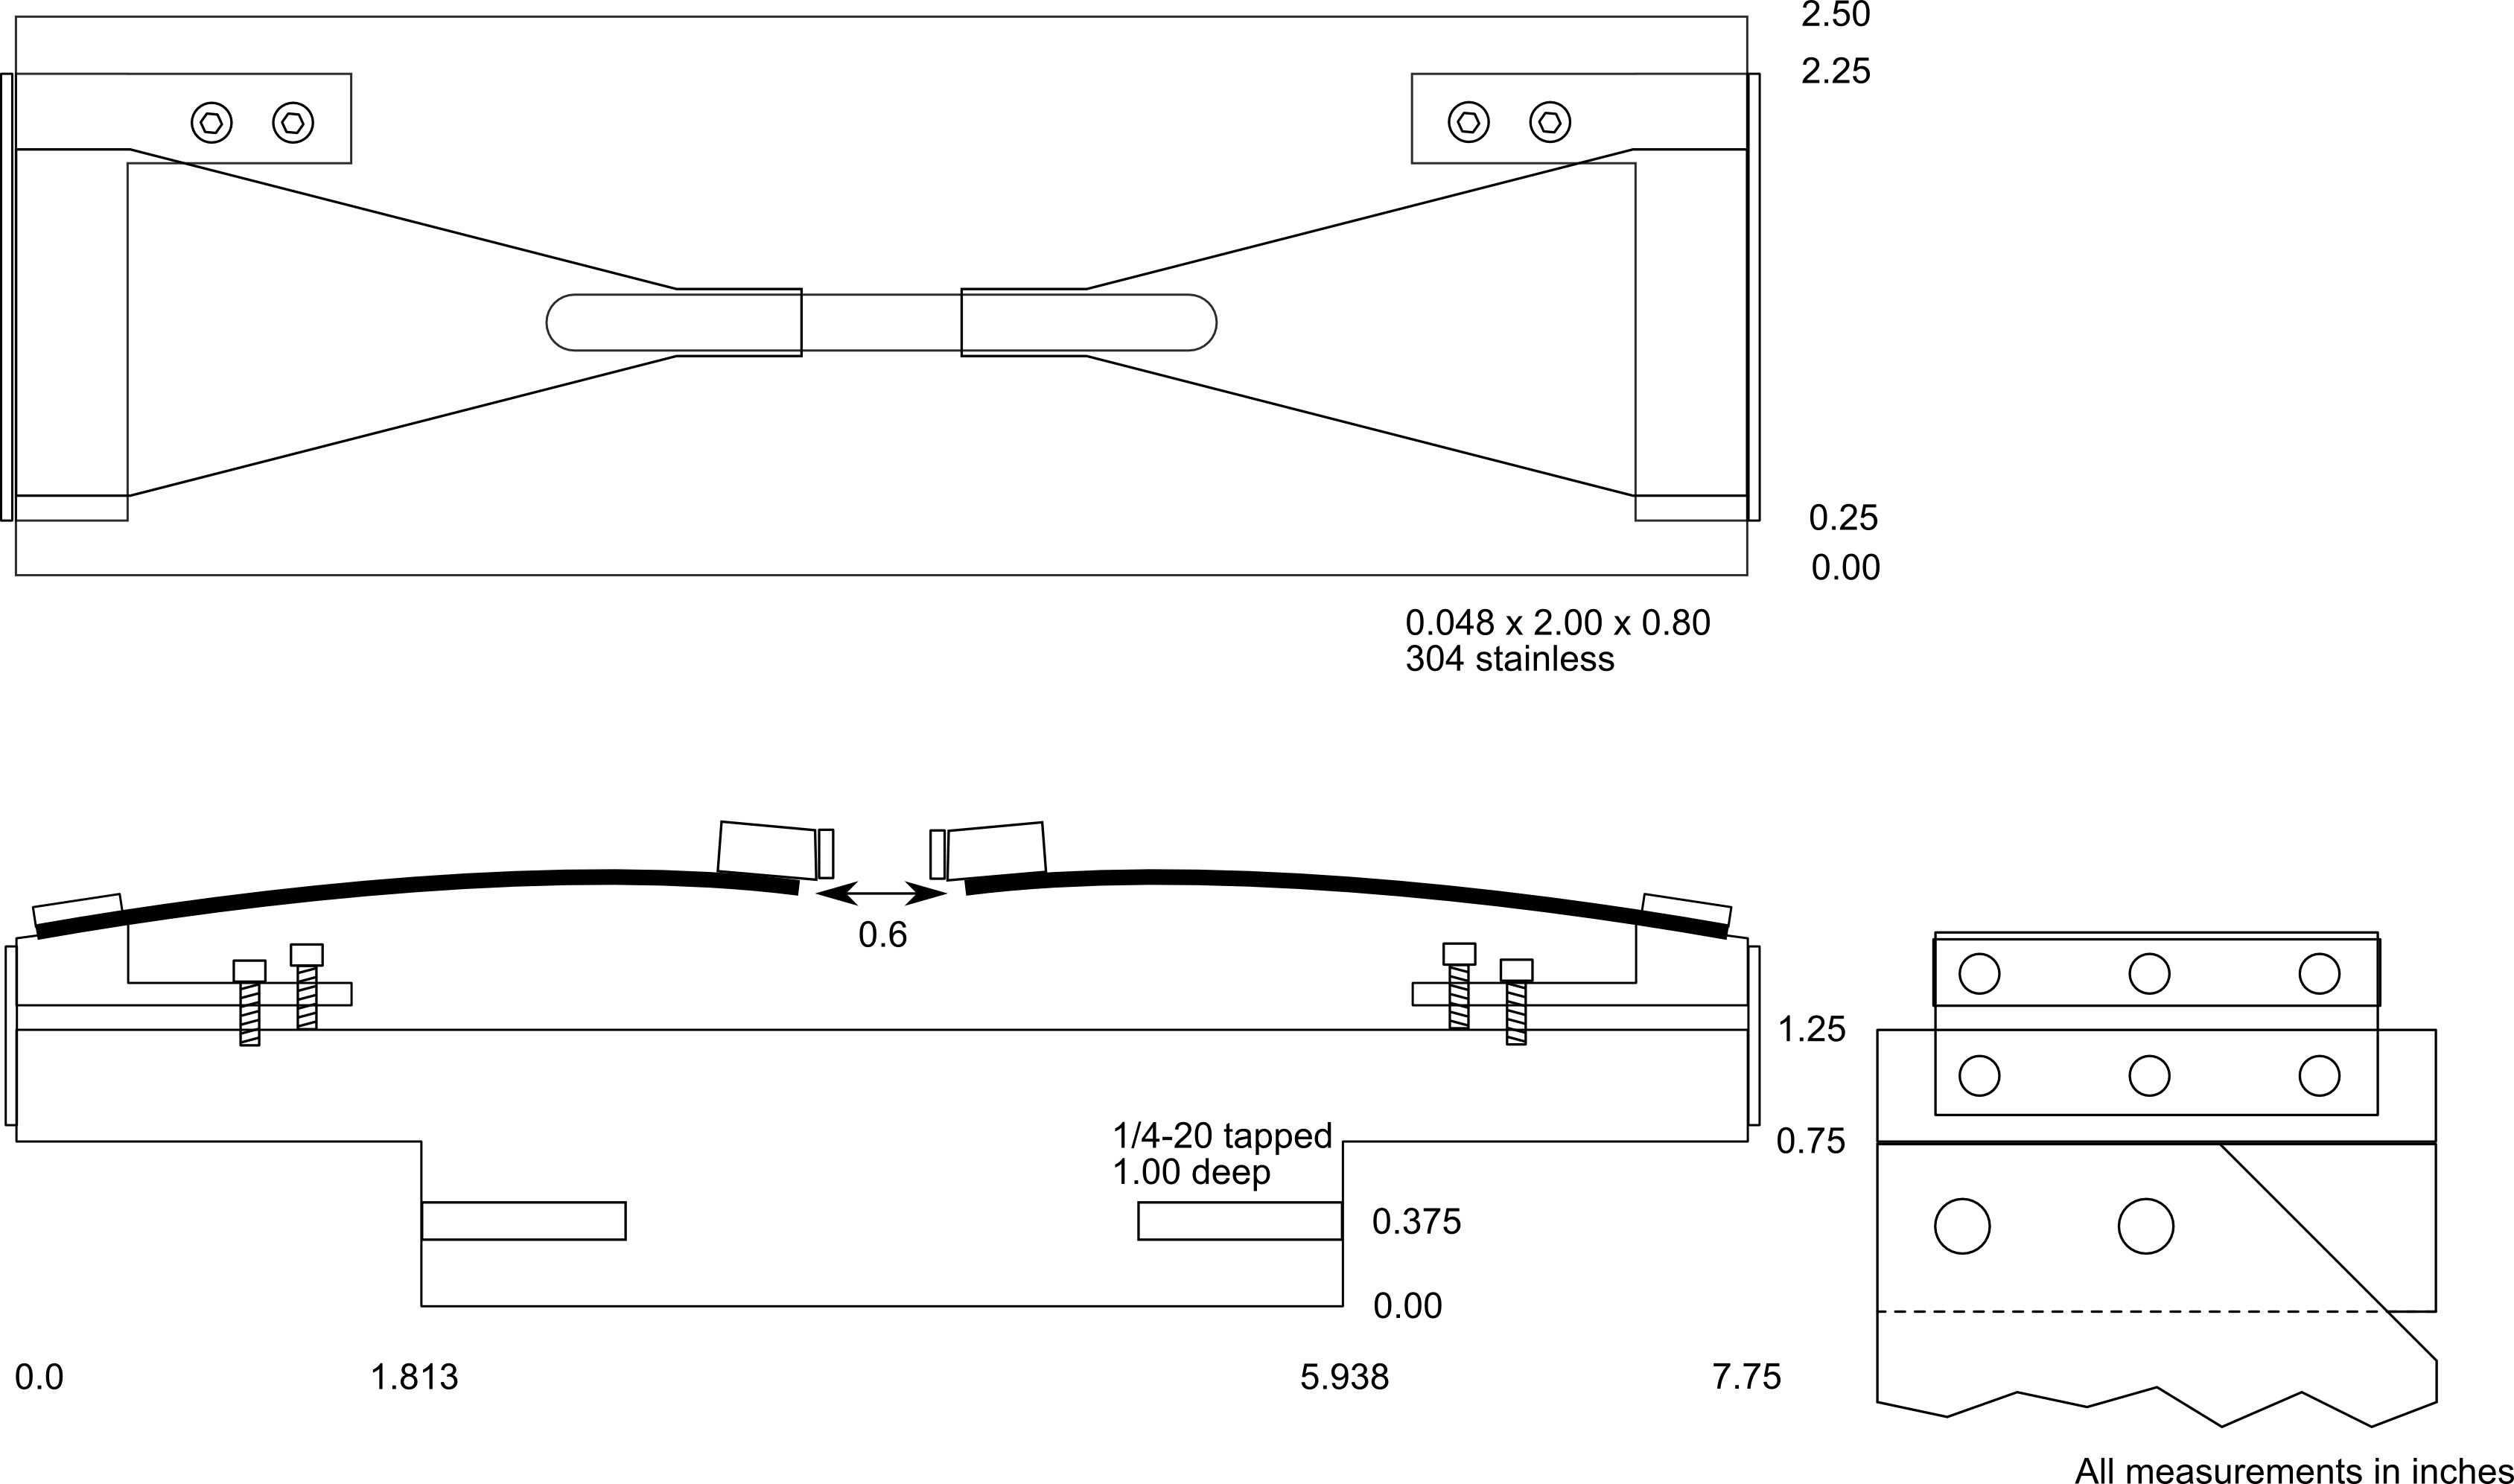
\includegraphics[width=\textwidth, angle=90]{figures/suspensions/bb1.png}
	\caption[Small blade design]{Drawings for the small blade suspension modification to the SOS. The blade angle can be adjusted using the screws. This adjustment was used for fine adjustment of the optic height and rotation.}
	\label{fig:babyschematic}
\end{figure}
\section{OSEM diagonalzation}

To control the mass under vacuum, we use devices called OSEMs (Optical Sensing Electro-Magnets). These are devices (see fig. \ref{fig:osem}) that sense the position of an optic using magnets which are mounted on the optic. The magnet partially blocks light from an LED, so when it moves it causes changes in the voltage out from a photodiode. This signal is sent to the digital system, where it is converted into position, pitch, yaw, and side motion. Each of these degrees of freedom have specific filters applied to them, then the signals are converted back into the five sensor distances. Coils in the OSEM are driven accordingy, controlling the motion of the optic.

\begin{figure}[hp]
	\centering
		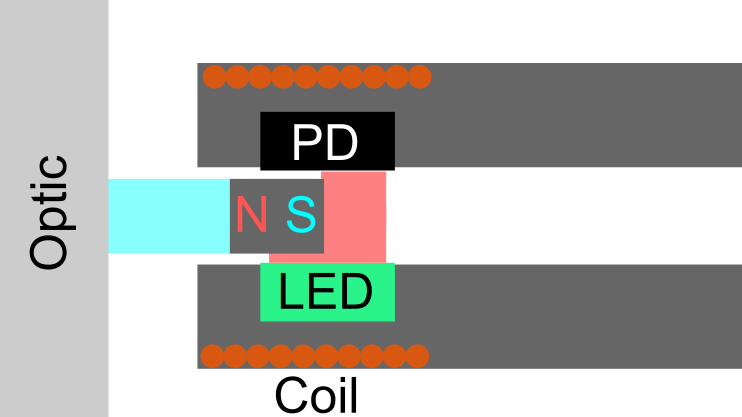
\includegraphics[width=.5\textwidth]{figures/suspensions/OSEM.png}
	\caption[OSEM diagram]{Layout of an Optical Sensing Electro-Magnet (OSEM). Optic motion is sensed when the magnet changes the amount of light from the light emitting diode (LED) that gets to the photodiode (PD). The coils can be driven to move the magnet and thus the optic.}
	\label{fig:osem}
\end{figure}

The hardest part to get right when using OSEMs is to properly diagonalize them so that you can push in the standard degrees of freedom (i.e. position, pitch, yaw, and side). This is accomplished in two steps, along with some sneaky meter-to-radian conversion. 

First, we diagonalize the input matrix. An ideal input matrix should look like table \ref{tab:idealDiag}. The input values are converted to micrometers before they get to this matrix. This matrix then converts the measurements to position and side measurements in $\mu m$ and pitch and yaw measurements in $\mu rad$ (the angular conversion is dependent on the fact that the magnets are mounted in a 4.94 by 4.94 cm square). Thus a change of $1 \mu m$ the upper left (UL) sensor is counted as : $.25 \mu m$ position, $-10.1 \mu rad$ in pitch, $10.1 \mu rad$ in yaw, and no change in side.

\begin{table}[hp]
\centering
\begin{tabular}{| c | c | c |c | c | l}
\bf{UL}& \bf{UR} & \bf{LR}  & \bf{LL} & \bf{SD}\\ \hline
  .25 & .25 & .25 & .25 & 0 &position ($\mu m$)\\
 -10.1 &-10.1 & 10.1 & 10.1 & 0 &pitch ($\mu rad$)\\
  10.1 &-10.1 &-10.1 & 10.1 & 0 &yaw ($\mu rad$)\\
  0 & 0 & 0 & 0 & 1 &side ($\mu m$)\\ \hline
\end{tabular}
\caption[Ideal diagonalization]{Ideal input matrix. The sensor inputs (in $\mu m$) are multiplied by the coefficients to get position of the mass in two directions (position and side) and the orientation of the mass (pitch and side). The coefficient for the angular measurements is calculated from the distance (1.945 in) between the magnets mounted on the mass.}
\label{tab:idealDiag}
\end{table}

However, due to OSEM alignment, machining defects, suspension inaccuracy, etc. the ideal matrix is not the most effective. Thus, we have a method for diagonalizing the matrices.

We drive one OSEM and look at the transfer function between that and all of the other OSEMs. We can determine from this the different modes (pos, pit, and yaw) by looking at the phase differences between the four back OSEMs (UL UR LL LR) at resonances. After this, we orthogonalize based on the coupling of each mode to the five osems. Here we have one interesting note: the position mode that we see is actually the pendulum mode, which is a combination of the pitch and position modes of the mass. The coupling scales inversely with the pendulum length.

\begin{figure}[p]
	\centering
		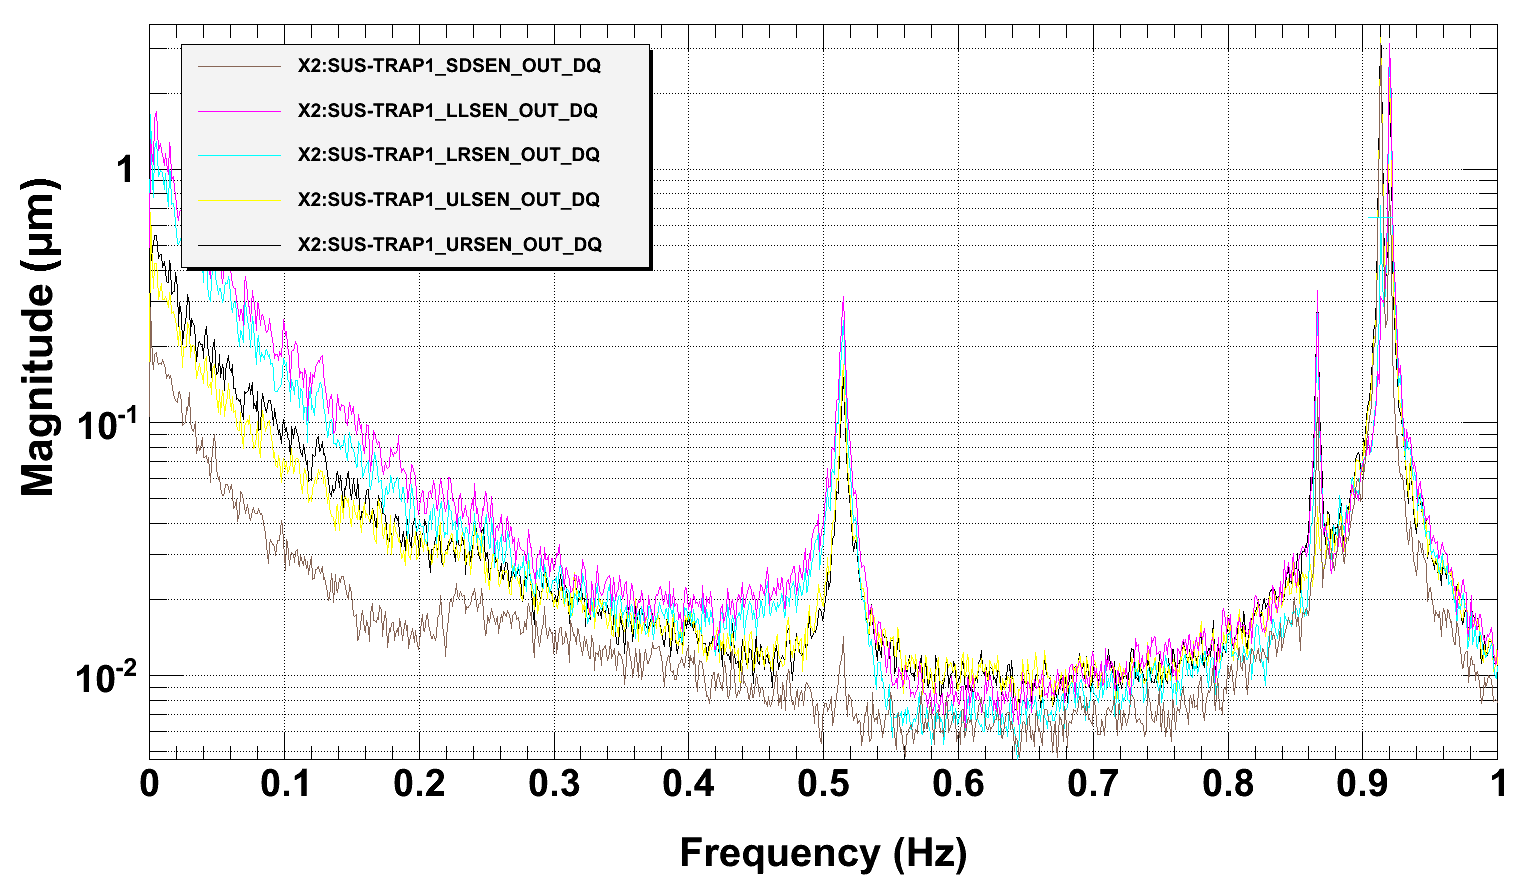
\includegraphics[width=.95\textwidth]{figures/suspensions/trap1spec.png}
	\caption[Input coupler spectrum]{Spectrum showing the modes of the input coupler.  Modes from low to high are: Pitch (0.511 Hz), Yaw (0.866 Hz), Side (0.911 Hz), and Position (0.918 Hz). }
	\label{fig:trap1spec}
\end{figure}


Once we have the input matrix set, we diagonalize the output matrix. We close the loops and drive each degree of freedom with a slow signal, then measure the responses in each of the (properly diagonalized) sensors. We subtract out the drive to the not desired degrees of freedom to determine the output matrix. 
%
%\begin{figure}[p]
	%\centering
	%\caption[Diagonlization noise comparison]{Plot showing the nosie before and after diagonalization}
	%\label{fig:diagNoise}
%\end{figure}

%\Chapter{Control Loops}
%\label{ch:controlloops}
%There are several control systems of note in an optical trapping setup. The subcarrier servo controls the accousto-optic modulators (AOMs) which take light from the carrier and frequency shift it to create the subcarrier. The trap cavity control servo and digital system are responsible for locking the cavity and reading out the cavity transfer function.

\begin{figure}[htbp]%
\centering
\includegraphics[width=.8\textwidth]{figures/photothermal/layout3}%
\caption[Simplified optical spring layout]{There are two main control loops in an optical spring system. The first is the subcarrier servo, (green box, lower right) which detunes the subcarrier a set frequency from the carrier. The second controls the laser frequency and the trap cavity input coupler to lock the cavity.}%
\label{fig:controlLoopsSimple}%
\end{figure}

\section{Subcarrier Servo}
The goal of the subcarrier servo is to red detune the subcarrier beam a set frequency away from the carrier beam. 
The required frequency shift is roughly twice the cavity pole frequency. 
With the parameters of our experiment, our cavity pole frequency was about 140 kHz, and thus our required detuning was about 300 kHz. 
There are no easily available AOMs that work in that frequency range. 
Previous experiments \cite{Corbitt07} have overcome this by shifting an entire FSR plus the desired detuning, but the FSR of our cavity is about 2 GHz, which is above the range of standard AOMs. 

Thus we chose a difference frequency scheme with two AOMs frequency shifting in opposite directions to achieve small offset (~200kHz) within a single FSR.
This system is controlled by the subcarrier servo, which is designed to lock a VCO (voltage controlled oscillator) a set frequency away from a crystal oscillator. The is accomplished through two mixers and some feedback, as shown in figure \ref{fig:subcarrierservo}.

We use directional couplers to get low-power signals from both the 80 MHz crystal oscillator and the VCO so that the majority of the power is driving the AOMs, maximizing the optical power going into the first order mode. 
The signal from the oscillator is mixed with the output of the VCO to produce a signal where the frequency is the difference between the two signals. 
This signal is then mixed with the desired offset frequency, set on the function generator, to give a low frequency error signal.
The error signal is passed through some filters in the servo, then fed into the VCO frequency modulation input.

\begin{figure}[htbp]%
\centering
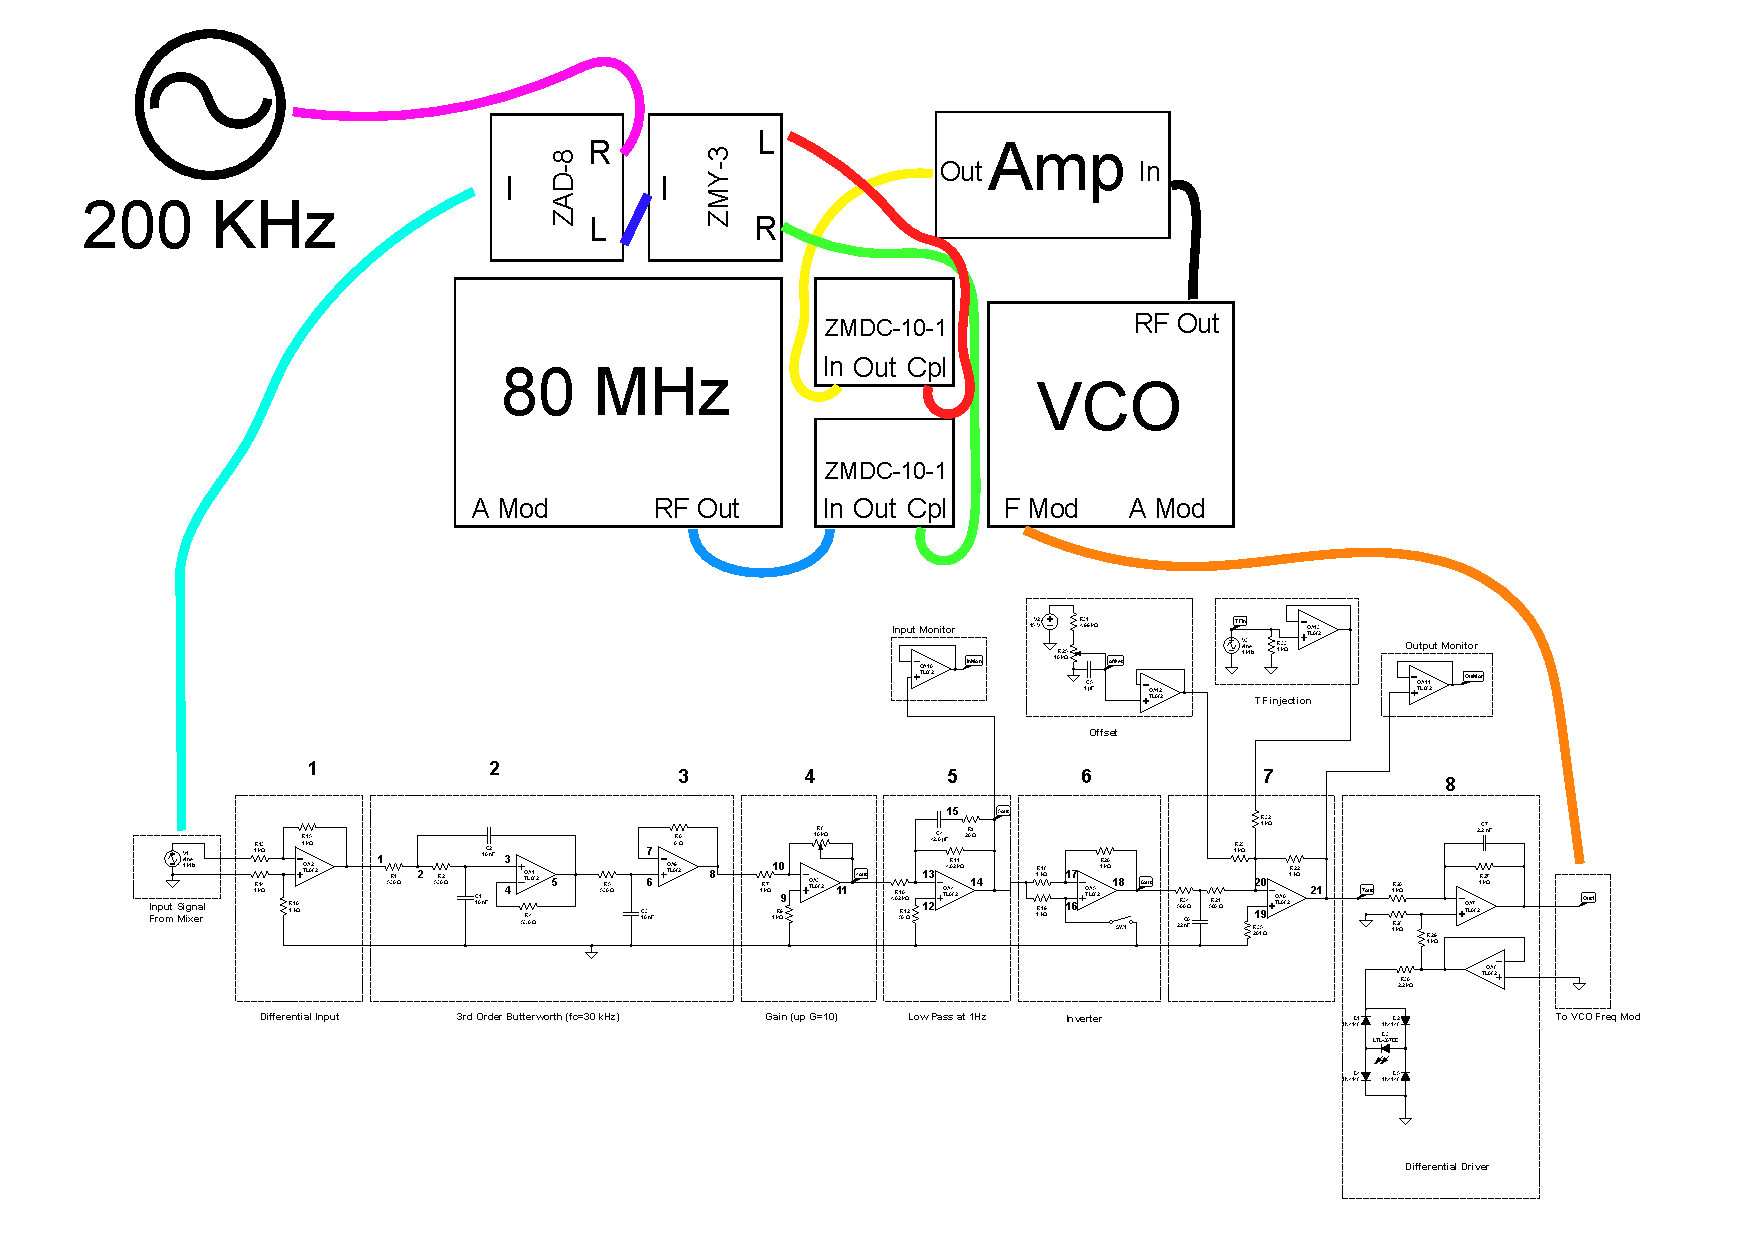
\includegraphics[width=1.2\textwidth,angle=90]{figures/controls/SubcarrierServo}%
\caption[Subcarrier Servo]{Subcarrier Servo diagram. The servo locks the VCO output to the 80 MHz oscillator output, offset by the function generator. The VCO and 80 MHz output signals are taken from the directional couplers (ZMDC-10-1), which output a majority of the power through the ``Out'' terminal to the AOMs. Those signals are fed through a mixer (ZMY-3), then the output is mixed again (ZAD-8) with the function generator (200 kHz).
The function generator can be tuned from roughly 50 kHz to 2 MHz.}%
\label{fig:subcarrierservo}%
\end{figure}

We typically monitor two spots in this system: The output of the fast mixer (ZMY-3) and the drive signal from the function generator (200 kHz on the diagram). When locked, the two should have the same frequency and be phase locked. The unity gain frequency of the locked system is about 2 kHz. below that, the servo should suppress frequency noise in the AOM drive (though it will not help for sensing noise). 

%\lab\lab2013\Subcarrier_servo\20130424_freq_noise

%\section{Introduction}
%
%We're going to take a single oscillator, and beat it against a time delayed version of itself to figure out the phase noise.  This method should work for any oscillator, though there are `dead spots' in the spectrum due to resonance that we have to be careful about.
%
%Let's cover some variables...
%
%\begin{itemize}
%\item Oscillator Frequency $f_{osc} = 80 \mbox{MHz}$
%\item Speed of light in BNC cables $s = 0.66 c$
%\item Volt of mixer DC offset per radian of phase: $g_{rad}=0.34 \mbox{V/rad}$
%\item Delay Cycles $n=3$ 
%\item Time delay $T=\frac{n}{f_{osc}}$
%\item Phase noise measurement frequency $f_{meas}=1 \mbox{kHz}$  
%\end{itemize}
%
%$$A e^{i(\omega t+\phi(t))}   \otimes B e^{i(\omega (t-T)+\phi(t-T))} = A(\omega) e^{i(\omega T+\phi(t)-\phi(t-T))} $$
%
%Our friendly spectrum analyzer does an FFT on it...
%
%$$\phi(\omega) (1-e^{i\omega T}) \approx \phi(\omega) i \omega T$$
%
%then we can ask ourselves, ``how accurately can I measure this noise?''  Assuming a spectrum analyzer noise floor of $1 \mbox{nV}/\sqrt{\mbox{Hz}}$
%
%$$\phi_{min}=\frac{1 \mbox{nV}}{\sqrt{\mbox{Hz}}} \frac{1}{g_{rad}}\frac{1}{2\pi f_{meas}T}$$
%$$=\frac{1 \mbox{nRad}}{0.34\sqrt{\mbox{Hz}}}\frac{f_{osc}}{2\pi (1\mbox{kHz})(n)}$$
%$$=\frac{1 \mbox{nRad}}{0.34\sqrt{\mbox{Hz}}}\frac{f_{osc}}{2\pi (1\mbox{kHz})(n)}$$
%$$=\frac{37}{n} \frac{\mu Rad}{\sqrt{\mbox{Hz}}}$$
%
%This is the smallest phase noise that we could measure for a given $n$.  Note that, with a wavelength of about 2.5 m, it is feasable to consider an $n$ up to perhaps 20.
%
%Next question is: how does phase noise affect our noise in the cavity (in $m/\sqrt{\mbox{Hz}}$)?
%
%$$ f_n(\omega)=\frac{1}{2\pi}\frac{d}{dt}\phi_n(\omega) = \frac{\omega}{2\pi} \phi_n$$
%
%$$FSR+f_n=c/(2L+x_n)\approx\frac{c}{2L}\left(1-\frac{x_n}{2L}\right)$$
%
%current nosie estimate is $10^{-17}m/\sqrt{\mbox{Hz}}$
%
%$$f_n = \frac{c}{2L}\left(1-\frac{x_n}{2L}\right)-FSR = 1.3\times 10^{-7}$$
%
%$$\Delta x \approx \frac{\lambda_0^2}{2L}$$ distance between peaks in an FSR
%
%so our lower bound in phase noise measurement should be below
%
%$$\phi_n = f_n \frac{2\pi}{\omega}= 8.4\times10^{-10} rad/\sqrt{\mbox{Hz}}$$

\subsection{Measuring frequency noise}

We are going to look at the spectrum of the oscillators near 80 MHz to figure out the amount of frequency noise from these oscillators.  We're mostly concerned with the frequency noise in the 1 kHz band around the peak.

We begin by assuming that all voltage noise is phase noise (no change in the amplitude).  This method gives an upper limit to the noise in the system.

In the following discussion, $\omega_m$ is a measurement frequency and $\omega_c$ is the carrier frequency.

We expect the voltage output to be $V(t) = V_0 e^{i(\omega_c t + \phi(t))}$, where $\phi(t)$ is the noise in the system.

In the frequency domain,

\begin{equation}
\delta V(\omega_m) = V_0 \delta \phi(\omega_m) = \frac{2\pi V_0}{\omega_m} \delta f(\omega_m).
\label{eq:VofOmega}
\end{equation}

It is important to note that we need to sum the effects of the noise at the carrier plus 1 kHz and the carrier minus 1 kHz to get the total frequency noise.

\begin{equation}
\delta f(\omega_m)= \frac{\omega_m \delta V(\omega_m)}{2 \pi V_0}.
\label{eq:deltafSCS}
\end{equation}


We can now calculate the effect of this frequency noise on our optical trap cavity length $\delta x$.  $f_L$ is the laser frequency.

\begin{equation}
\delta x = \frac{L}{f_L} \delta f = 2.66\times10^{-16} \delta f.
\label{eq:deltax}
\end{equation}

%The noise budget gives a noise floor of $10^{-17}$, so to get in under that, we need $\delta f <<\frac{1}{26.6}$.


\subsection{Results}

With the subcarrier servo locked at approximately 200 kHz, the noises we measure are:

80 MHz Oscillator: frequency noise $5.4\times 10^{-3} \frac{\mbox{Hz}}{\sqrt{\mbox{Hz}}}$.  Position noise $1.4\times 10^{-18} \frac{\mbox{m}}{\sqrt{\mbox{Hz}}}$.

VCO: frequency noise $6.7\times 10^{-2} \frac{\mbox{Hz}}{\sqrt{\mbox{Hz}}}$.  Position noise $1.7\times 10^{-17} \frac{\mbox{m}}{\sqrt{\mbox{Hz}}}$.

Both of these values are below the expectation of laser frequency noise at 1 kHz (about $2\times 10^{-15} \frac{\mbox{m}}{\sqrt{\mbox{Hz}}}$) , so that should be acceptable.

%These noise values are OK for the 80 MHz oscillator, but not so much for the VCO.  We suspect that the 200 kHz oscillator may be the culprit.


\begin{figure}[htp]
	\centering
		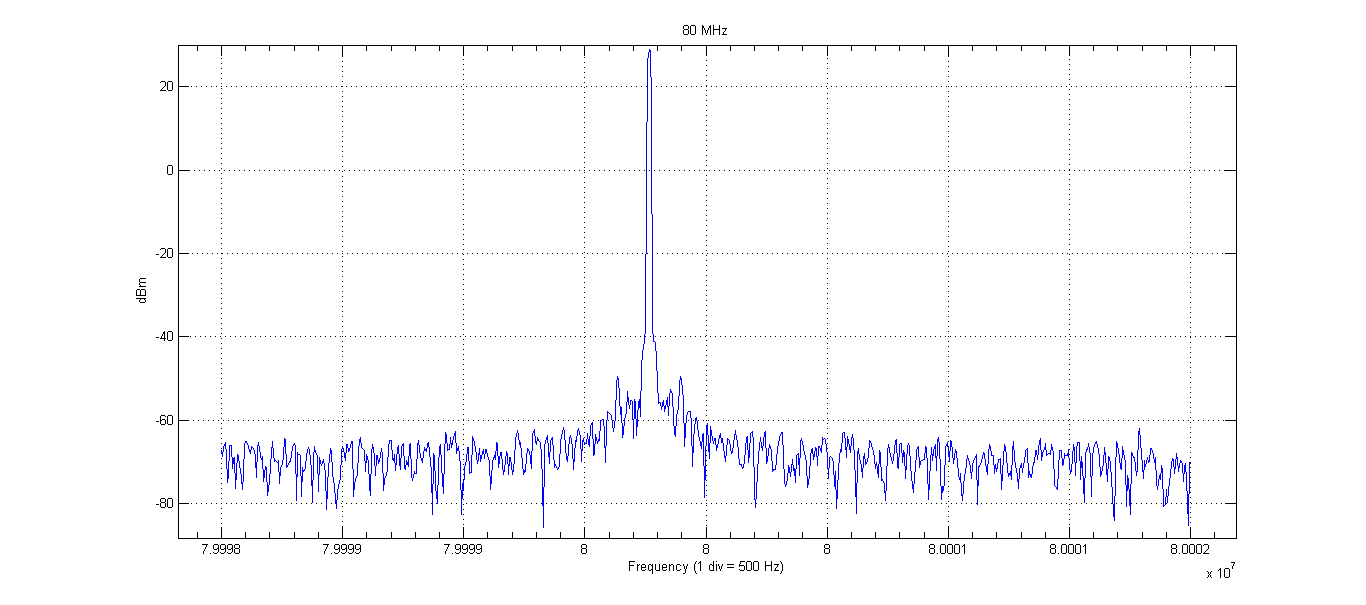
\includegraphics[width=\textwidth]{figures/controls/80.png}
	\caption[80 MHz oscillator spectrum]{Spectrum of the 80 MHz crystal oscillator around 80 MHz.}
	\label{fig:80}
\end{figure}

\begin{figure}[htp]
	\centering
		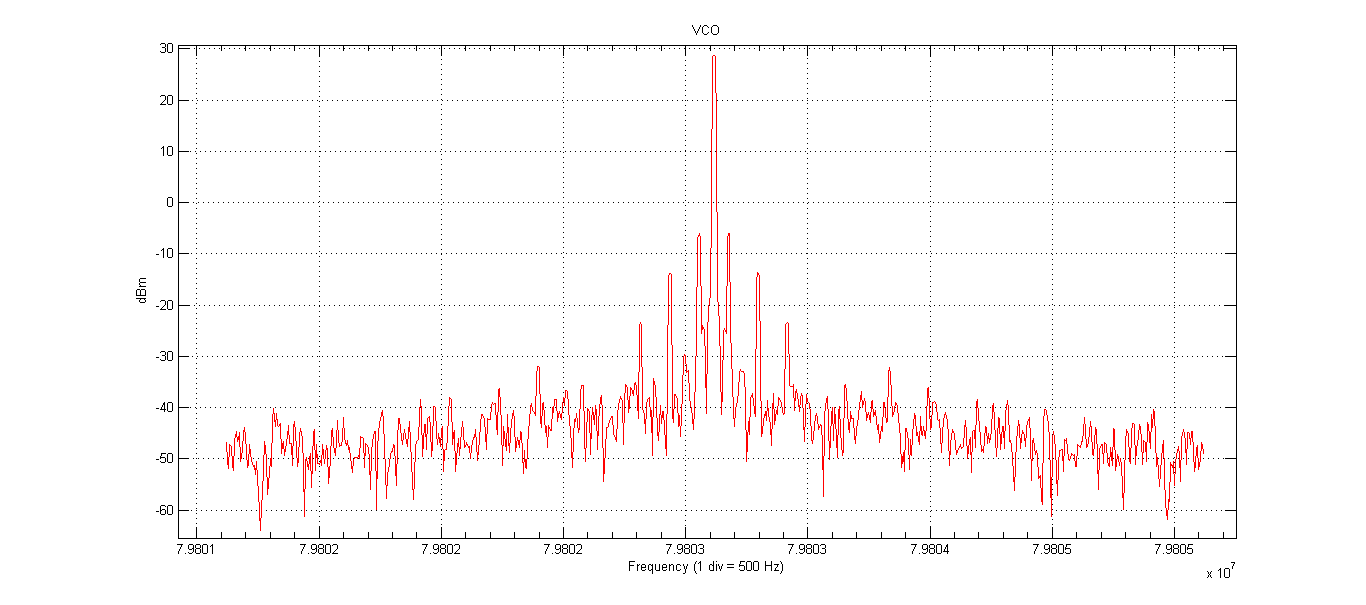
\includegraphics[width=\textwidth]{figures/controls/VCO.png}
	\caption[VCO spectrum]{Spectrum of the locked VCO. The sidebands are likely caused by the function generator.}
	\label{fig:VCO}
\end{figure}



\section{Cavity control loops}

\begin{figure}[htp]
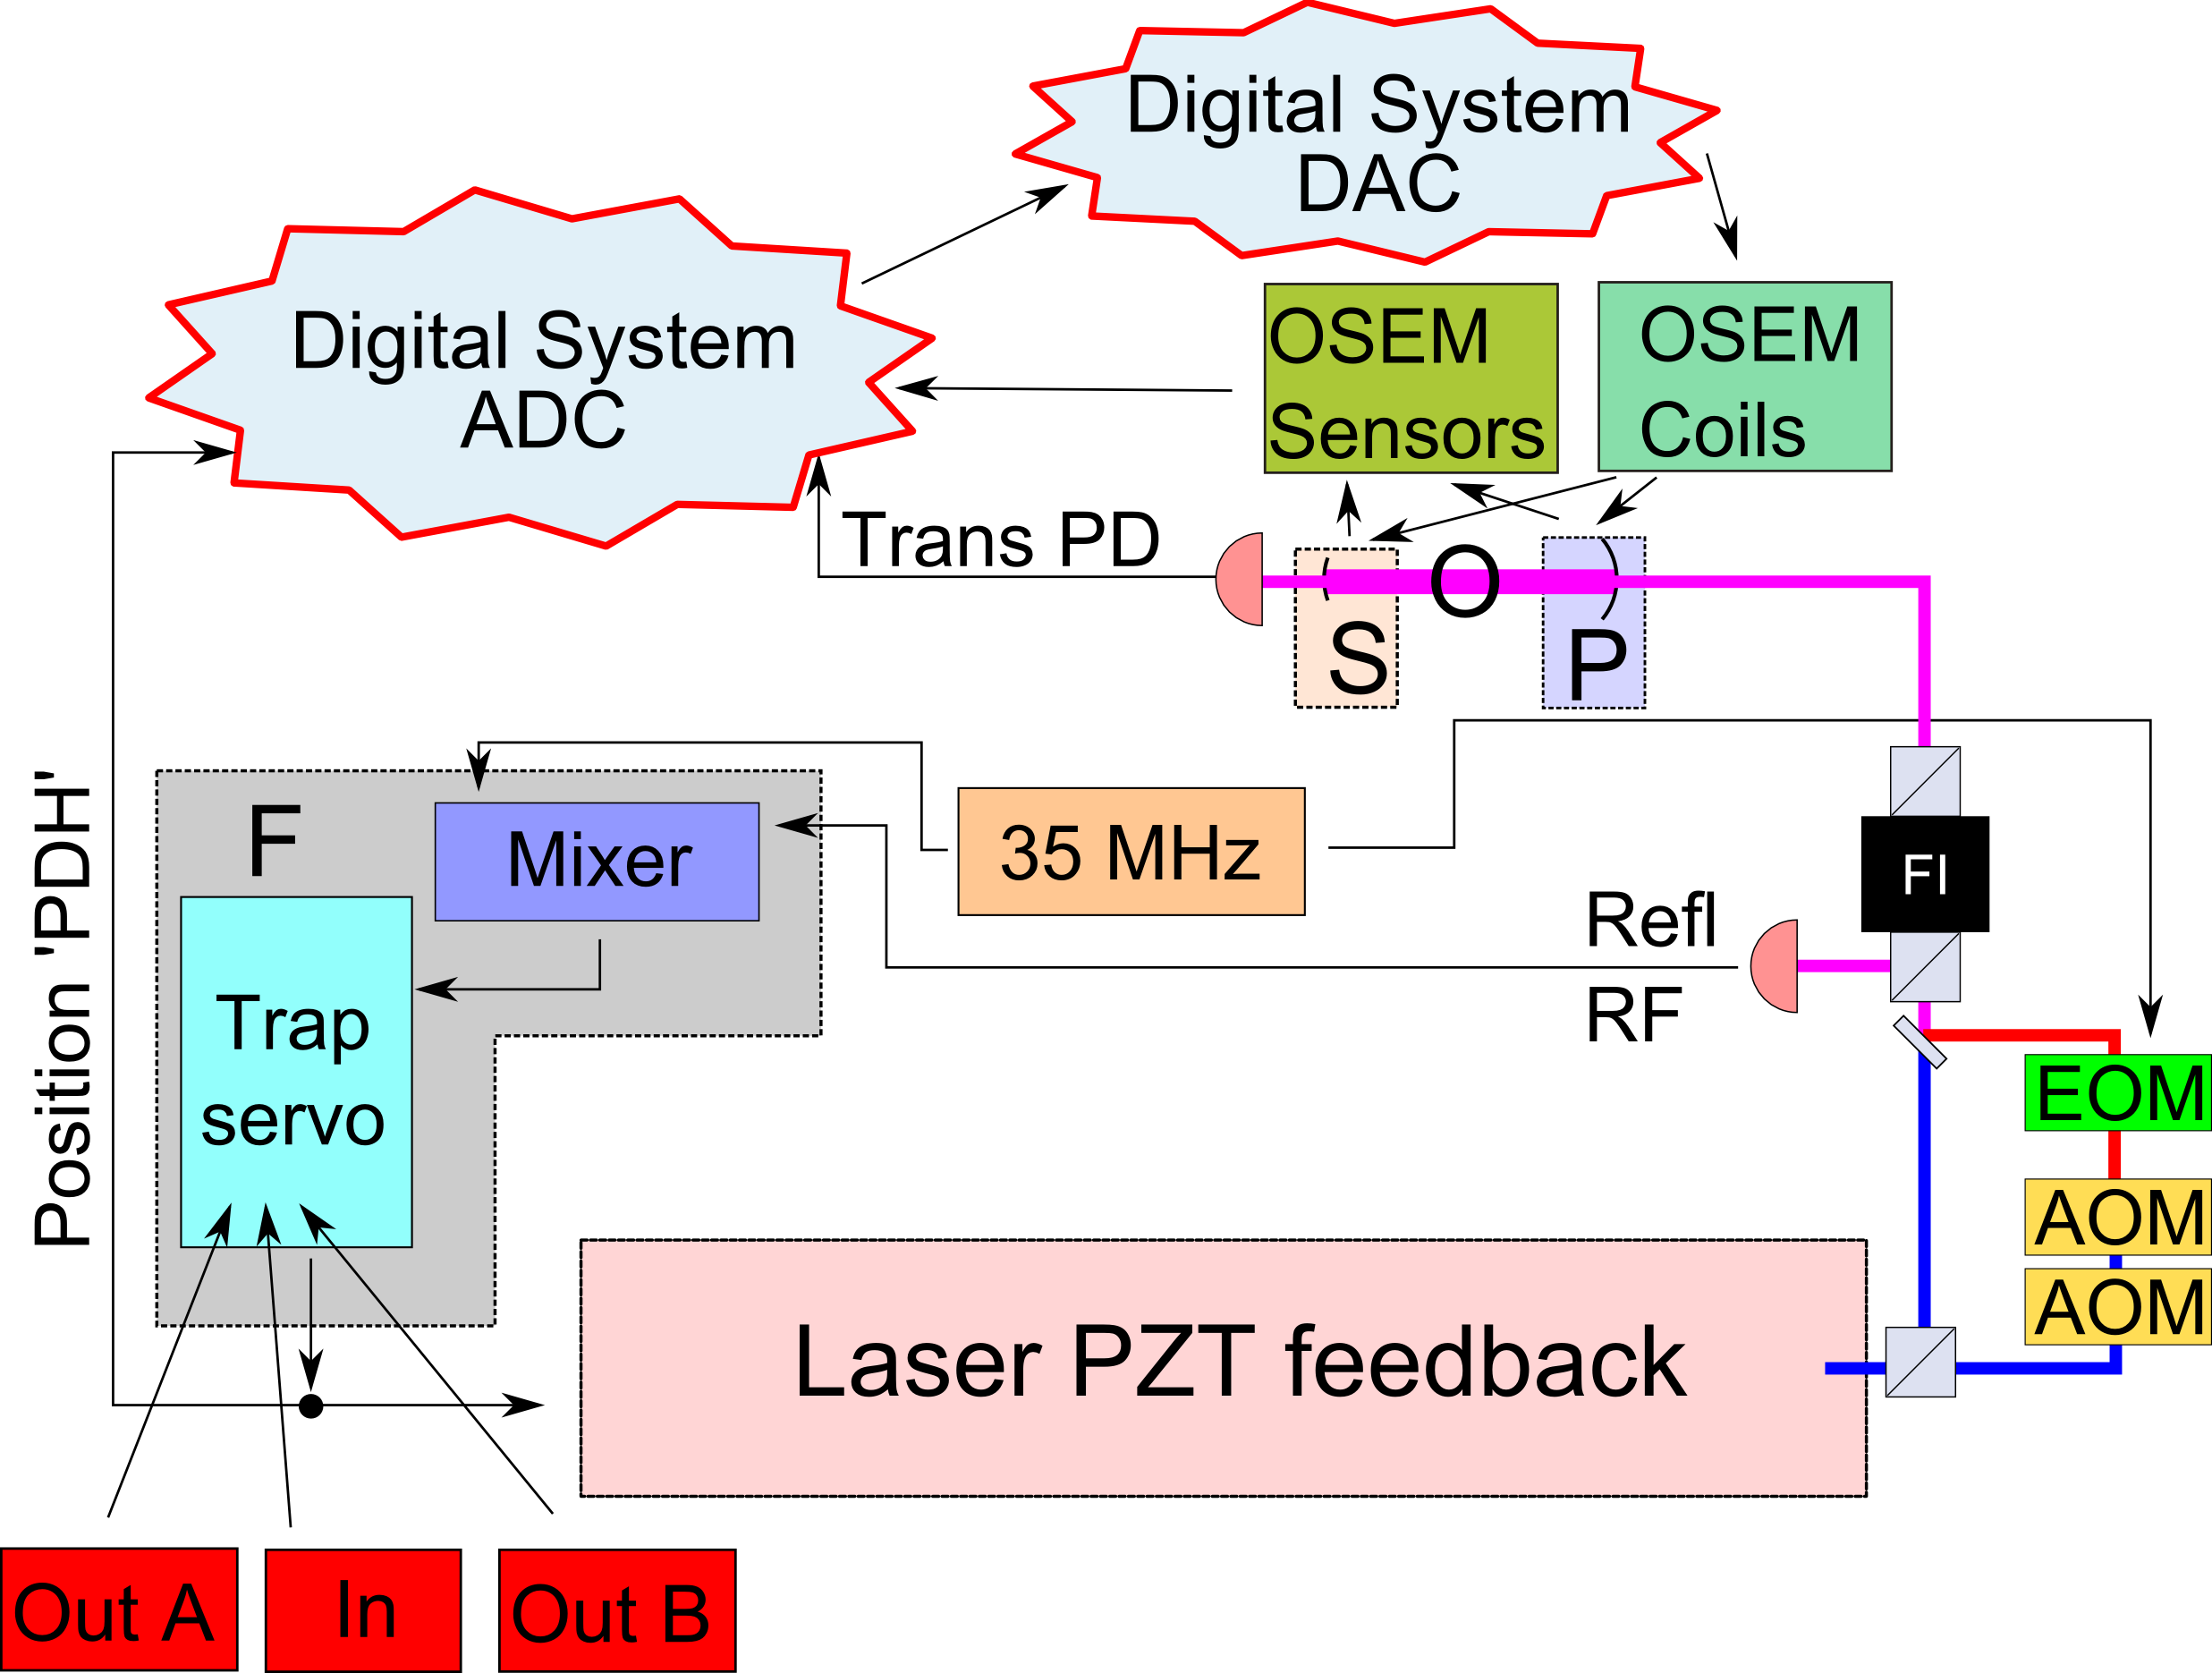
\includegraphics[width=475pt,angle=270]{figures/controls/traplockSimple.png}%
\caption{Analog parts of the locking loop. We lock the cavity (OS) using the PDH signal from the reflected RF photodiode (Refl RF). The feedback signal goes to the laser PZT for fast feedback and to the digital system for slow feedback to the OSEMs. We measure the open loop transfer function of the system by driving the ``In'' port, then measuring ``OutA'' divided by ``OutB''.}
\label{fig:traplock}%
\end{figure}

\begin{figure}[htp]
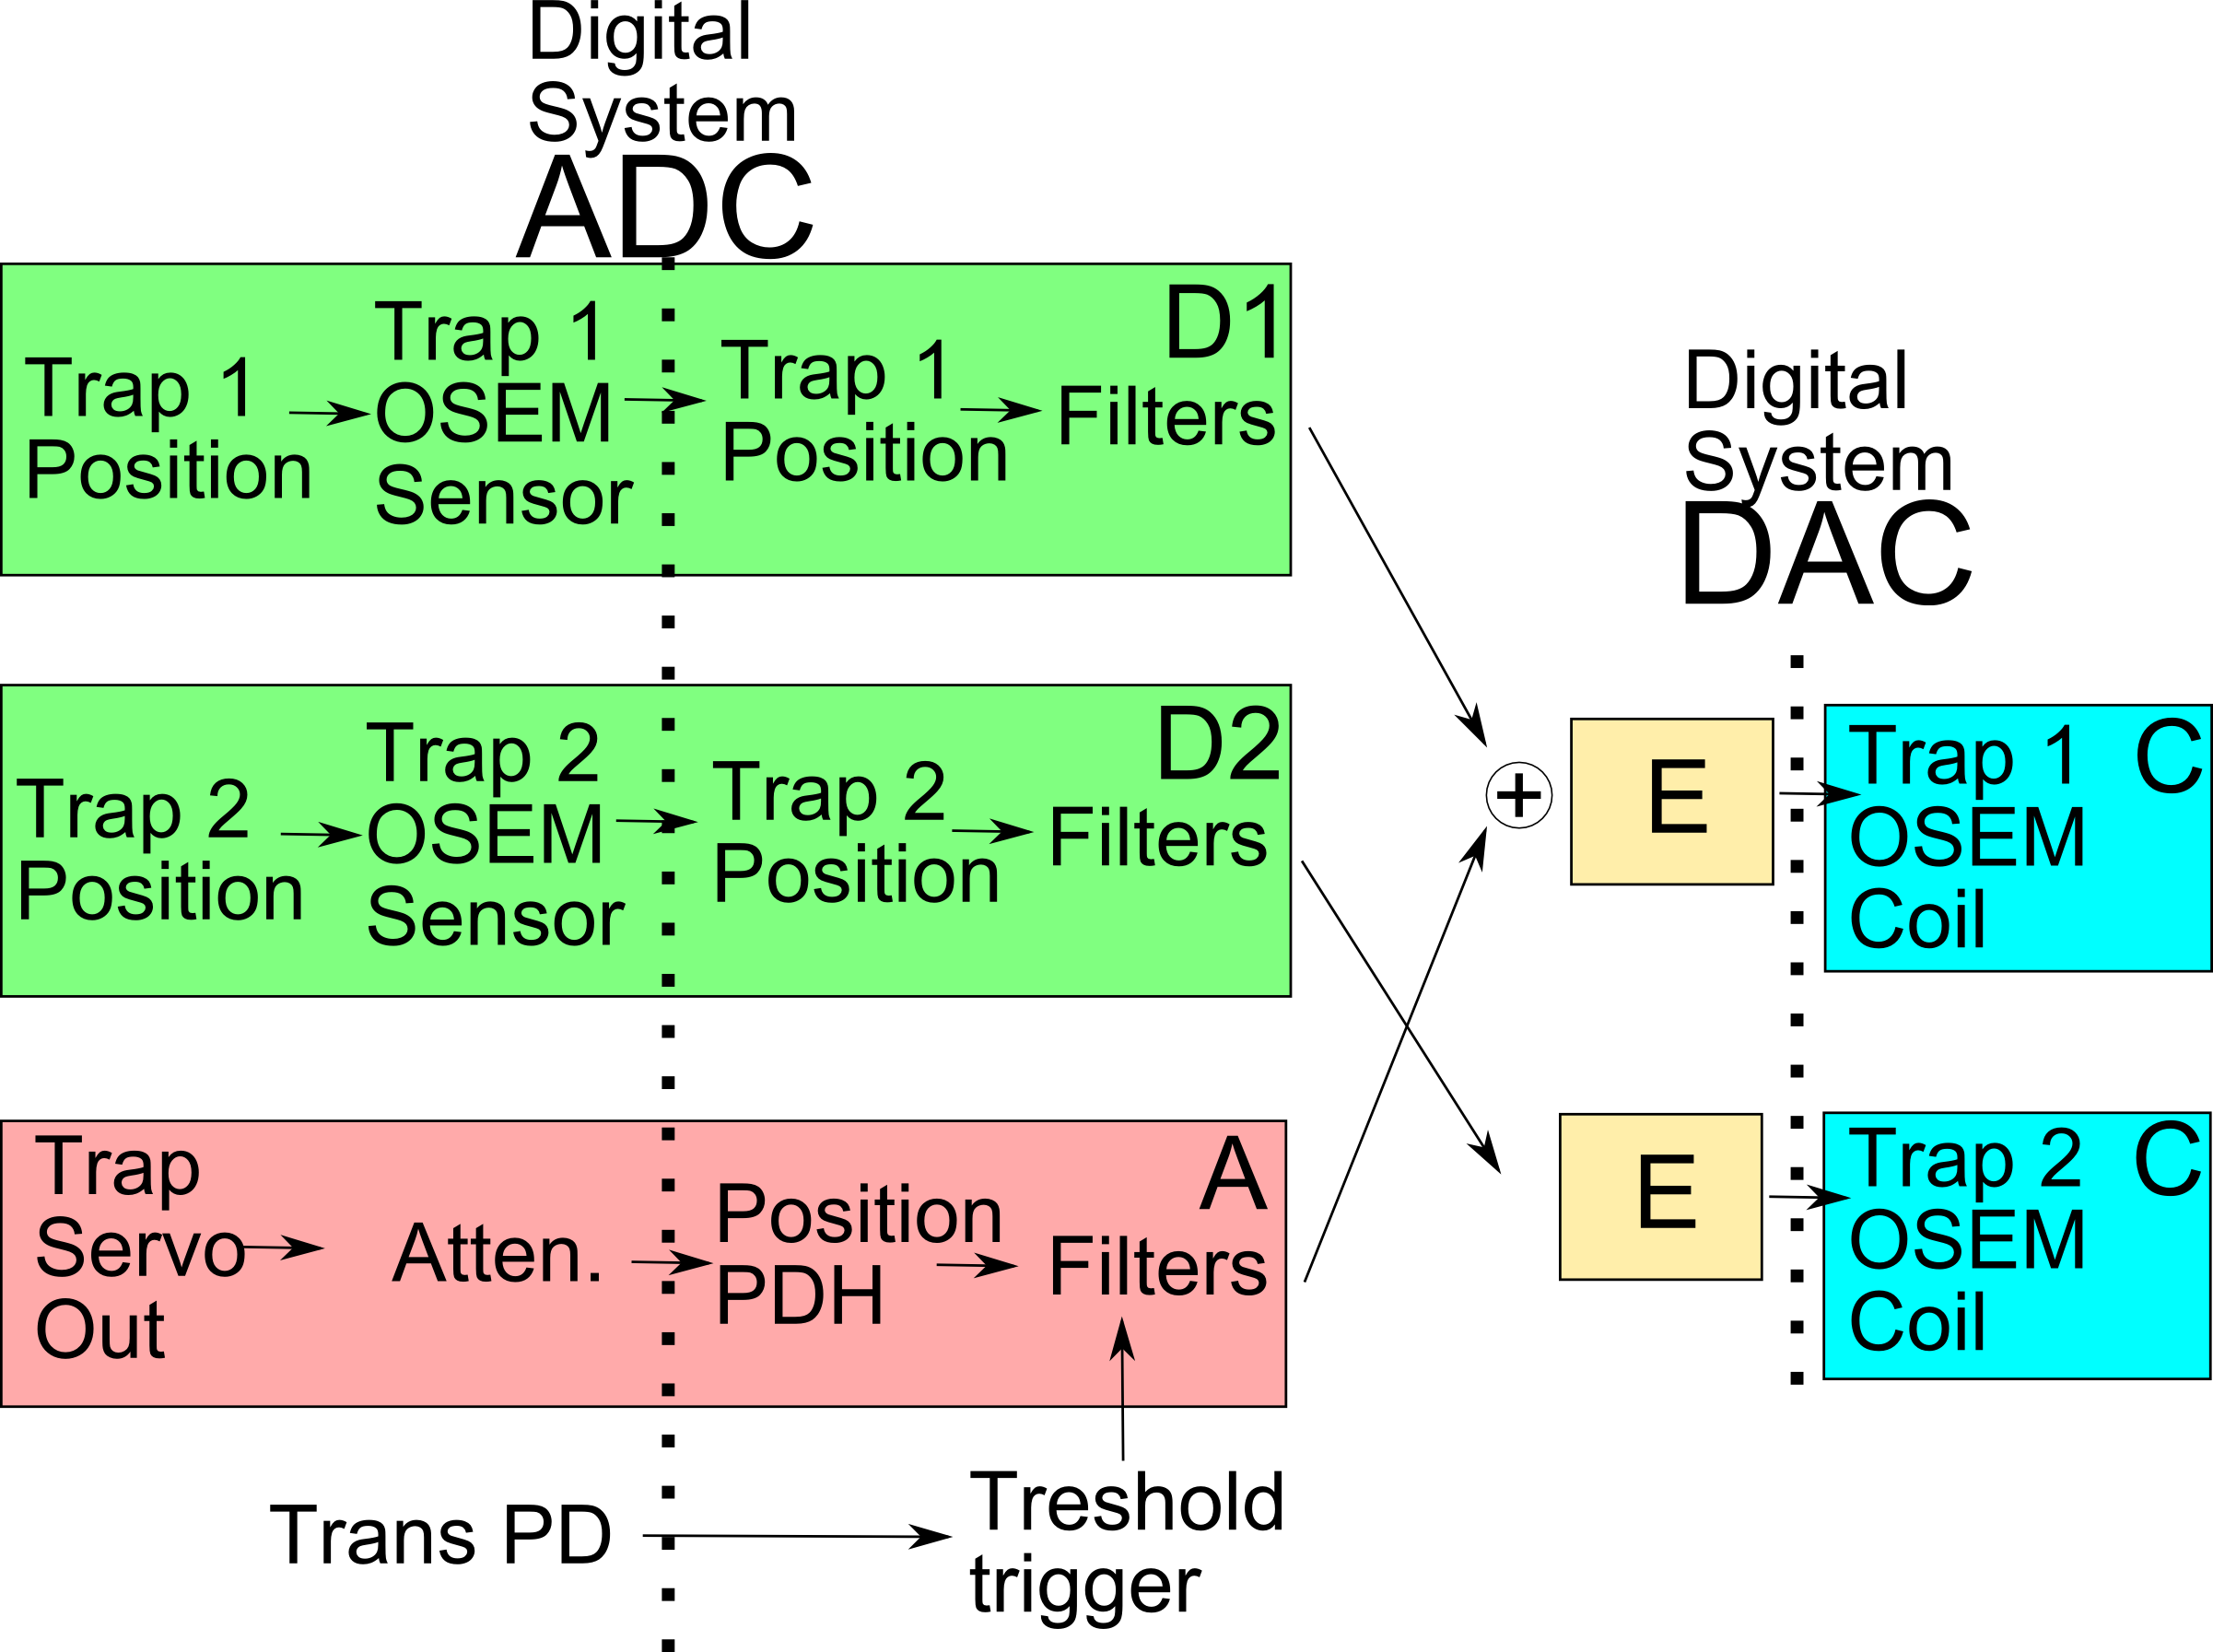
\includegraphics[width=\columnwidth]{figures/controls/traplockdig.png}%
\caption[Digital loops]{Digital parts of the locking loop. These parts are responsible for the slow feedback to the OSEM coils. The yaw and optical lever inputs are not relevant to the longitudinal trap.}%
\label{fig:traplockdig}%
\end{figure}


Here's a picture of the longitudinal trap as it stands.  In general terms, we have a cavity with position and laser feedback, which also has optical spring behavior.  Analog and digital loops are shown in figures \ref{fig:traplock} and \ref{fig:traplockdig}.

%You may notice that this layout drawing has an alphabet soup of sections and subsections. 
%I will now describe in excruciating detail what each of these things are and why we care.  


Each component has a letter associated with it, which represents the transfer function of the associated element. Each of the following sections describes an element and how it is calculated.
I am leaving out the input whitening on the analog side and the dewhitening on digital side.  They should cancel out every time, so we just leave them off.

Our goal is to be able to reconstruct the entire optical trap from the control point to the error signal.  In our measurements, we are using the injection input and the two test outputs of the Trap Servo board. Test out A serves as our error signal (OUT) and Test out B serves as our control signal (IN).  The injection happens between the two test outputs. The resulting open loop transfer function is plotted in figure \ref{fig:OLG}.
This is based on James Lough's  \cite{LoughThesis} model of the loop, which I have updated and repackaged.

%\begin{equation}
%\frac{F}{1-SO}\left[HLM+\frac{AECP+TCP}{1-PCED}\right]
%\label{eq:loop}
%\end{equation}

\begin{equation}
\frac{Out A}{Out B}=\left[FHLM+\frac{FAECP+FTCP}{1+PCED}\right]\frac{1}{1+SO}.
\label{eq:loop}
\end{equation}

There are several different parts to this equation, so we will take a moment to look at each term.  Every term in the numerator includes $F$, the Trap Servo. $FHLM$ is a loop involving the PZT drive of the laser.  $FAECP$ and $FTCP$ both rely on pushing the large mass around using the OSEM drive, but $FAECP$ does the drive through the digital system while $FTCP$ uses an analog connection. $PCED$ is the open loop transfer function of the active suspension damping for the large mass; note that this only affects the loops that are driving the large mass. $SO$ is the open loop transfer function of the optical spring acting on the small mirror, which is dependent on the separation between the two mirrors, rather than the absolute position of either.



%-360 is a product of two closed loops and one open loop.  The two closed loops are the optical spring, $(1-SO)^{-1}$, and the active seismic damping from the digital system to the OSEMs, $(1-PCED)^{-1}$.  The open loop is the sum of three paths: the feedback of the trap servo through the laser ($FHLM$), the feedback of the trap servo through the digital system to the OSEMs ($FAECP$), and the feedback of the trap servo directly to the OSEM drive ($FTCP$) 

\begin{figure}[htbp]
\centering
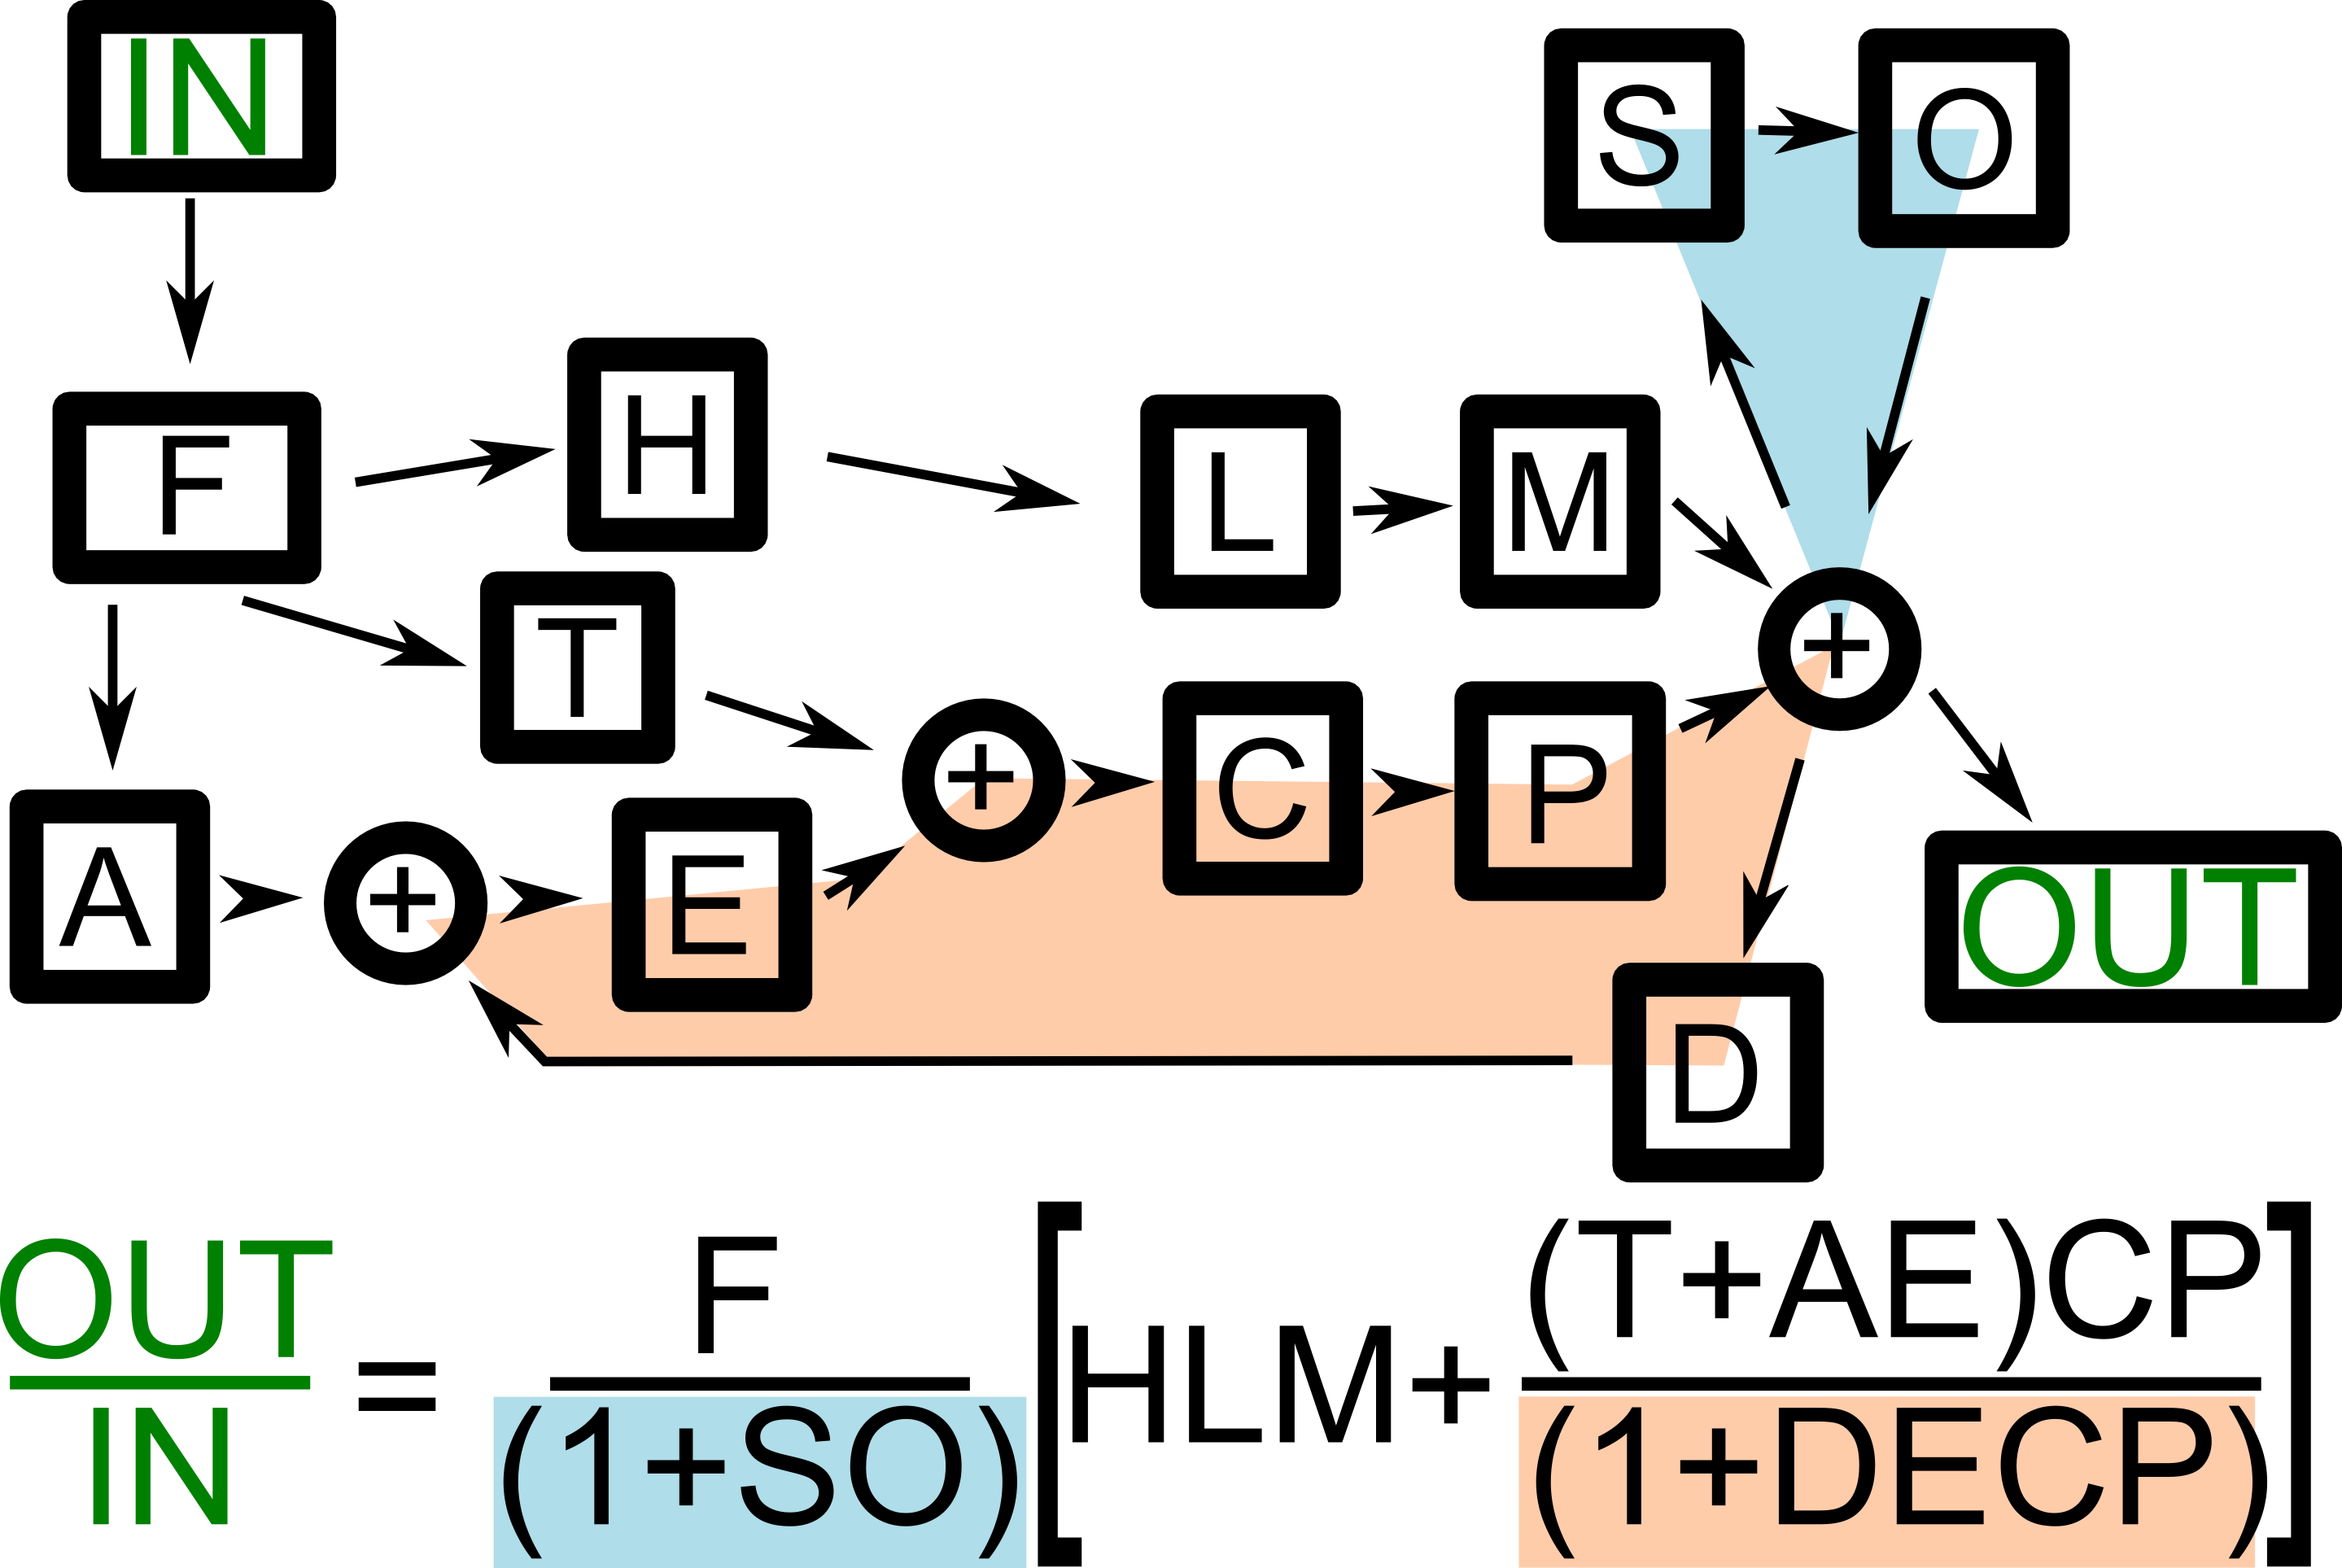
\includegraphics[width=\columnwidth]{figures/controls/blocks.png}%
\caption[Block diagram of the system]{Block diagram of the open loop transfer function for trap locking and operation. Two closed loops (OS and DECP) are highlighted in blue and red, respectively.}%
\label{fig:blocks}%
\end{figure}


%I'm using for reference Jim's code, TrapLoop.m, which is a Matlab class.  The code can be found in /lab/jim/newtrap. There is an example of the code in use, fitplots.m, in /lab/lab2014/TrapServo/20140423/



\subsection{A : Digital PDH feedback}

At the moment, this path has been disconnected because it was not required.  Thus we can set $A=0$.

%The input to this is the signal coming out of the Trap servo. The output is a drive signal which gets added into the OSEM drive of trap 1.  This box has a digital and an analog component.  In the analog section, the signal gets an attenuation $a = 95\Omega/2795\Omega$ via a votage divider.  After that, the signal enters the digital system, where we have the filters in the POS\_PDH\_FEEDBACK filter bank.  At the moment, the only active filter is a lowpass with a single pole at $10 \mbox{Hz}$. The -0.5 is related to the digital system input, the 40/3 is a gain set in the digital system, and the -7 is a fitting parameter.
%
%\begin{equation}
%A = a\frac{-10}{1+\imath f/(10 \mbox{Hz})}\frac{40\cdot (-0.5)\cdot-7}{3\cdot}\left[\frac{\mu\mbox{N}}{\mbox{mV}}\right]\cdot \frac{1000(\mbox{mV/V})}{10^6(\mu\mbox{N}/\mbox{N})}
%\label{eq:A}
%\end{equation}

\subsection{C : OSEM coils}

The OSEM coils convert voltage from the DAC into force on the large mirror via the OSEMs.  We have a factor of 4 in the numerator because there are 4 OSEMs acting on the mass.  The constant ($4.91793\times 10^{4}$ V/N) comes from a measurement made in October 2013 and recorded in the SUGWG logbook (entry number 439).

\begin{equation}
C = \frac{4}{4.91793\times 10^{4}\mbox{ V/N}}.                               
\label{eq:C}
\end{equation}


\subsection{D1 and D2 : Digital feedback based on optic motion}
The input to each of these blocks the is motion of a single optic relative to the OSEMs. The OSEMs put out a current proportional to the position of the mass, which is digitized.  The output is a drive signal which gets added into the OSEM drive of trap 1 and trap 2, respectively.  The position measurements from each optic have filters applied from the TRAP1\_SUSPOS and TRAP2\_SUSPOS filter banks. In D1, we have an AC coupling filter(Z: 0, P: 0.5), a highpass (Z: 1, P: 100), and a fourth order Chebychev lowpass filter at $200\mbox{Hz}$ with $1\mbox{dB}$ of passband ripple (P: $67.3977\pm\imath81.4946$, $27.9074\pm\imath196.677$ G: -0.891251).  There is also a gain of 10, which includes the filter gain, the conversion of position of the optics relative to the OSEMs into voltage, and the conversion from volts to meters in the digital system. See fig. \ref{fig:D}. 

From the Matlab code:

\begin{verbatim}
    tf = (1i*freq - 0) .* (1i*freq - 1)...
        ./ (1 + 1i*freq / 0.5)...
        ./ (1 + 1i*freq / 100)...
        ./ (1 + 1i*freq / (67.3977+1i*81.4946))...
        ./ (1 + 1i*freq / (67.3977-1i*81.4946))...
        ./ (1 + 1i*freq / (27.9074+1i*196.677))...
        ./ (1 + 1i*freq / (27.9074-1i*196.677))...
        .* -0.891251...
        .* Dgain;
\end{verbatim}


We do not consider the effects of D2 because we are not putting any active drive through it. Thus it will not shape the loop as drastically as D1. The coupling between the mirror position and the ring position drops off drastically ($f^{-2}$) above the position resonance of the glass suspension ($\approx 18\mbox{ Hz}$). As we improve the lock, we expect that we will be able to reduce or even remove active feedback on the ring.

\begin{figure}[htbp]
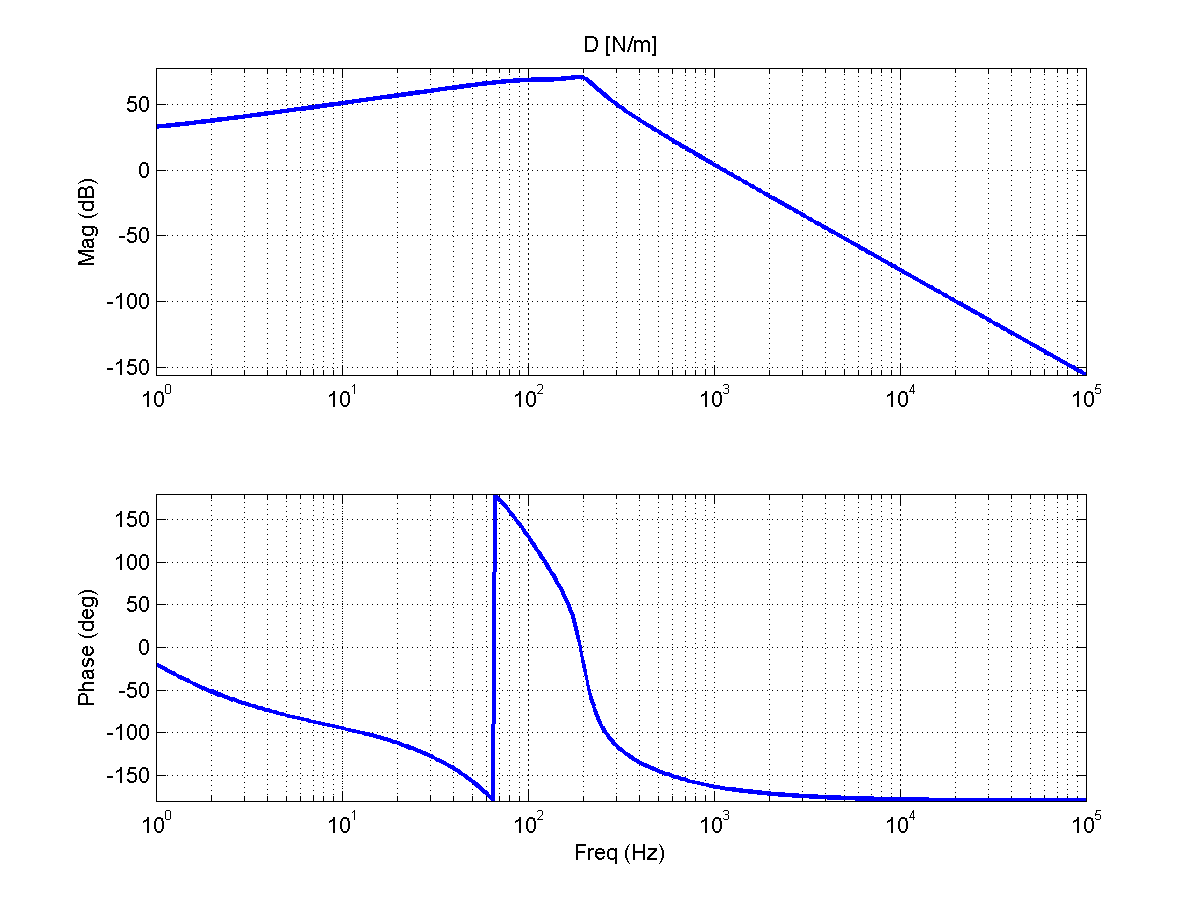
\includegraphics[width=\columnwidth]{figures/controls/D.png}%
\caption[D1 transfer function]{D1, the transfer function from the position of optic 1, the input coupler, to a digital drive force. }%
\label{fig:D}%
\end{figure}

\subsection{E : Force to volts}

The digital system converts the force output of digital filters into volts so that it can be sent out of the digital system to the OSEMs. We include a factor of 4 because we have 4 OSEMs.  Note that $CE = 1$.


\begin{equation}
E = \frac{1}{4} 4.91793\times 10^{4}\mbox{V/N}.
\label{eq:E}
\end{equation}

\subsection{F : Trap PDH servo}

This is the transfer function of the Trap Servo, the RF photodiode, and the mixer.  Input to this is the cavity length, read out through the PDH method. The output is a voltage. The variable `mxrpd,' which is the conversion from cavity length to the voltage output of the mixer, is dependent on power, cavity mode matching, and the PDH readout at the mixer. mxrpd, measured at full power, just below the oscillation point, is about $10^9$ V/m. See fig. \ref{fig:F}.  At the moment, we are only using the 100 Hz integrator. This has been modeled completely with the `Analog' library developed by Stefan Ballmer, rather than calculating the algebraic expressions. 

%in /software/matlab/analog.


\begin{figure}[htb]
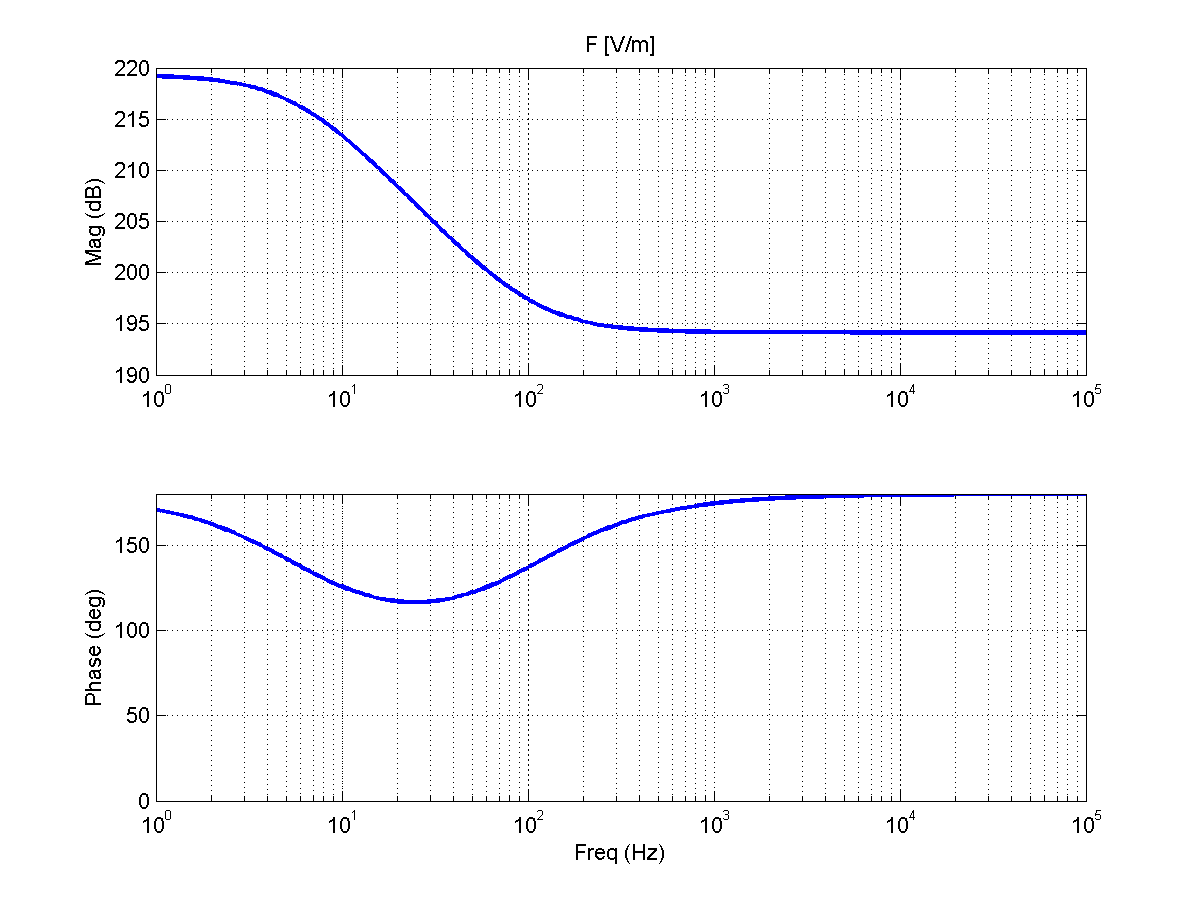
\includegraphics[width=\columnwidth]{figures/controls/F.png}%
\caption[Calculated trap servo TF]{Calculated trap servo TF. The main components are a 1 kHz lowpass filter and a user-adjustable gain.}%
\label{fig:F}%
\end{figure}

\subsection{P : Pendulum}

The pendulum transfer function of the large mass converts a force to a displacement in the position direction.  The resonant frequency is $f_L = 1.4 \mbox{Hz}$ and the Q factor is about 200. The mass of the input coupler is $m_L = 300$ g.

\begin{equation}
%P = \frac{1}{m_L (2 \pi f_L)^2} \frac{1}{\left(1 - \left[\frac{f}{f_L}\right]^2\right)}
P = \frac{1}{4 \pi^2\left[m_L (f_L^2-f^2)+\frac{iff_L}{2Q}\right]}.
\label{eq:P}
\end{equation}

\begin{figure}[htb]
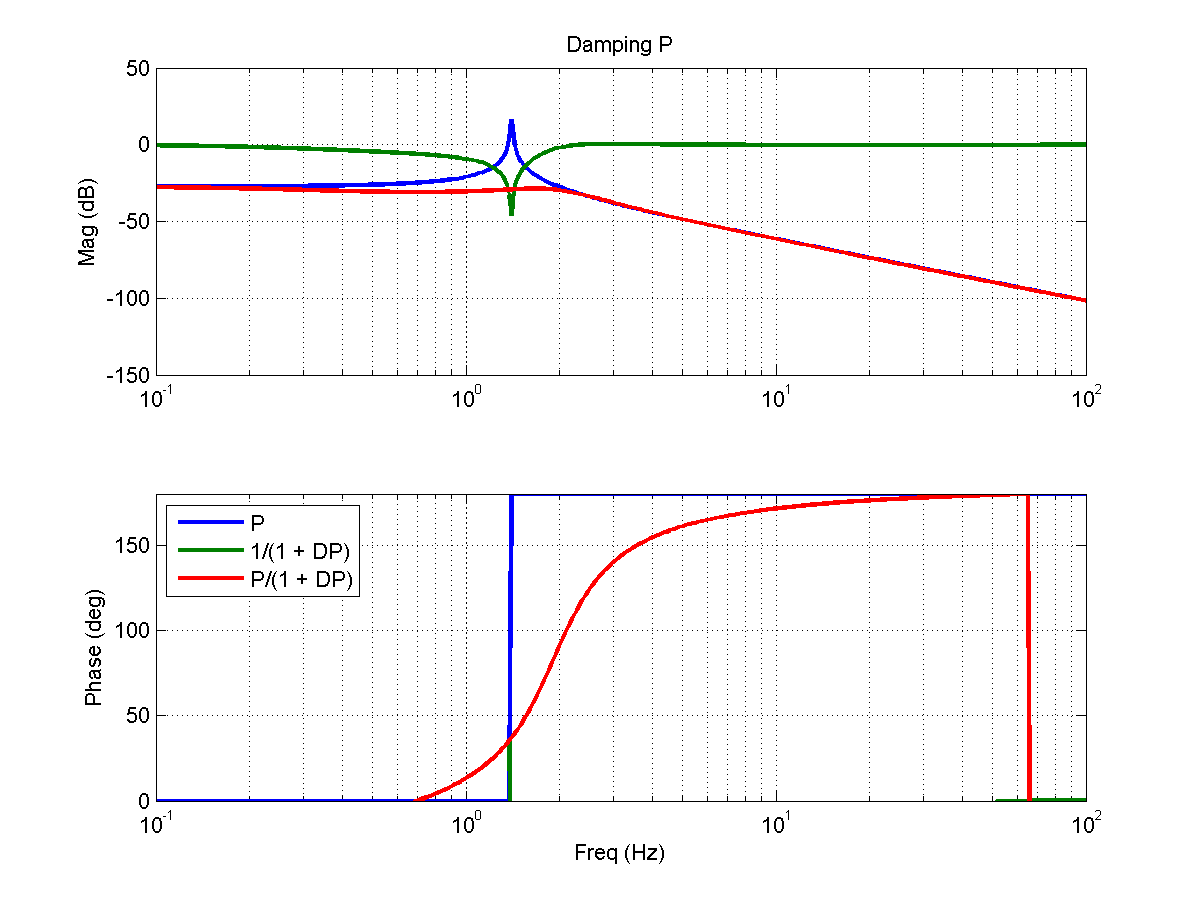
\includegraphics[width=\columnwidth]{figures/controls/P.png}%
\caption{Damped large mass pendulum transfer function.}%
\label{fig:DPloop}%
\end{figure}

\subsection{S : Suspension spring}

The glass suspension connects the small optic to the ring; it acts as a high-Q spring. An optical lever is used to damp oscillation modes other than the position mode. It converts a force to a displacement in the position direction.  The resonant frequency of the suspension is $f_s = 18 \mbox{ Hz}$ and the small mass is $m_s = 0.41 \mbox{ g}$.

\begin{equation}
S = \frac{1}{m_s (2 \pi f_s)^2}\frac{1}{\left(1 - \left[\frac{f}{f_s}\right]^2\right)}.
\label{eq:S}
\end{equation}

\subsection{O : Optical spring}

The optical spring has a transfer function that looks very much like that of a physical spring. Depending on detunings and power ratio, we should see stable or unstable behavior. One such transfer function is plotted in figure \ref{fig:O}.  We should note that optical losses before the cavity have to be considered when determining the power in the cavity, as well as the cavity detuning and angular displacements of the mirrors.  At the moment we are calculating this using Finesse \footnote{gwoptics.org/finesse/}.

\begin{figure}%
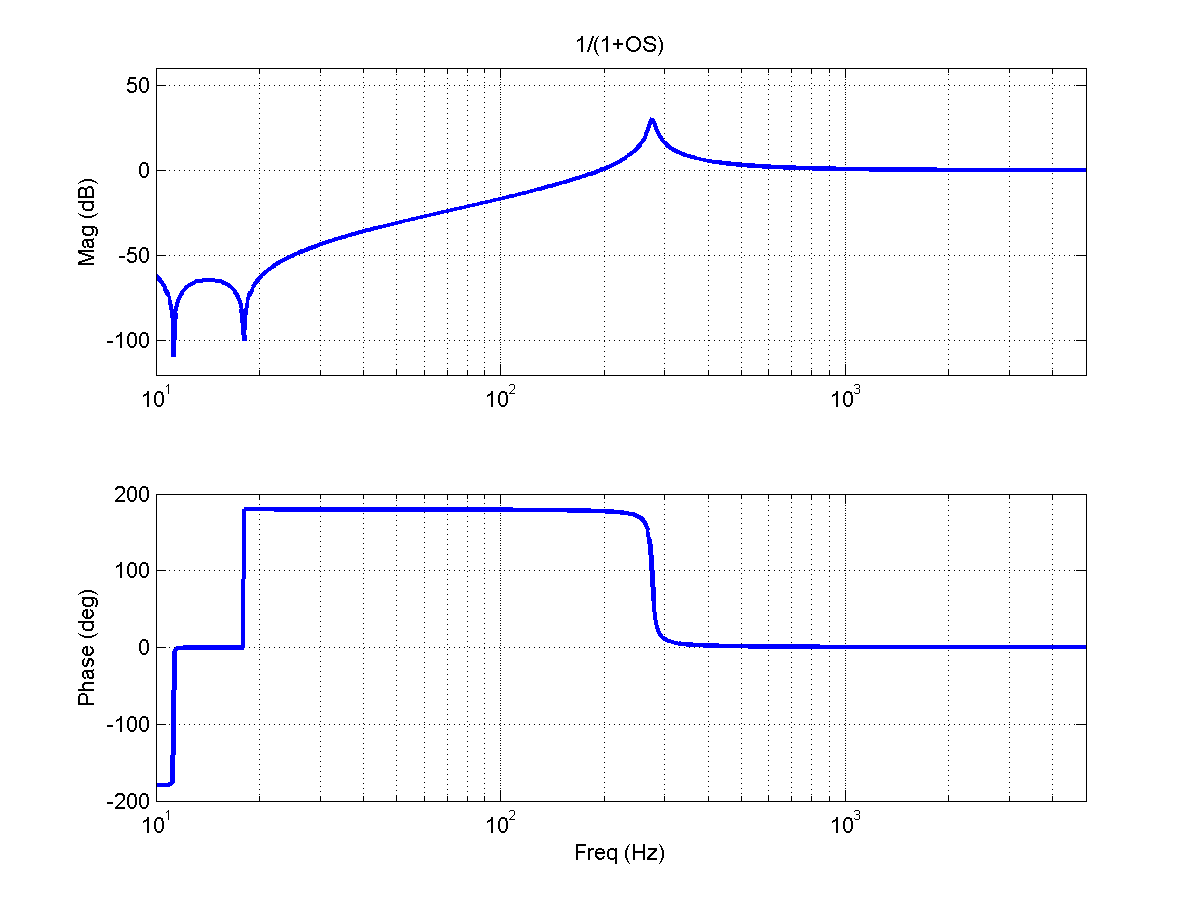
\includegraphics[width=\columnwidth]{figures/controls/O.png}%
\caption[Optical spring]{Plot of the closed loop behavior of the optical spring and the glass suspension.  
%The 1 Hz position resonance will be suppressed by the digital system damping loop}
%\caption{Optical Srping.  Single model has a single spring with power of 38 mW and a detuning of 33 kHz.  Dual model has two beams, a carrier with 295 mW detuned 355 kHz, and a subcarrier with 41 mW power detuned 260 Hz.  }%
}
\label{fig:O}%
\end{figure}

Combining this spring constant with S in a closed loop gives us the behavior of the optical spring on the small mass, and thus cavity length.  Below, in equation \ref{eq:OS_CL}, is the effect of the optical and mechanical springs on changes in the cavity length.

%\begin{figure}%
%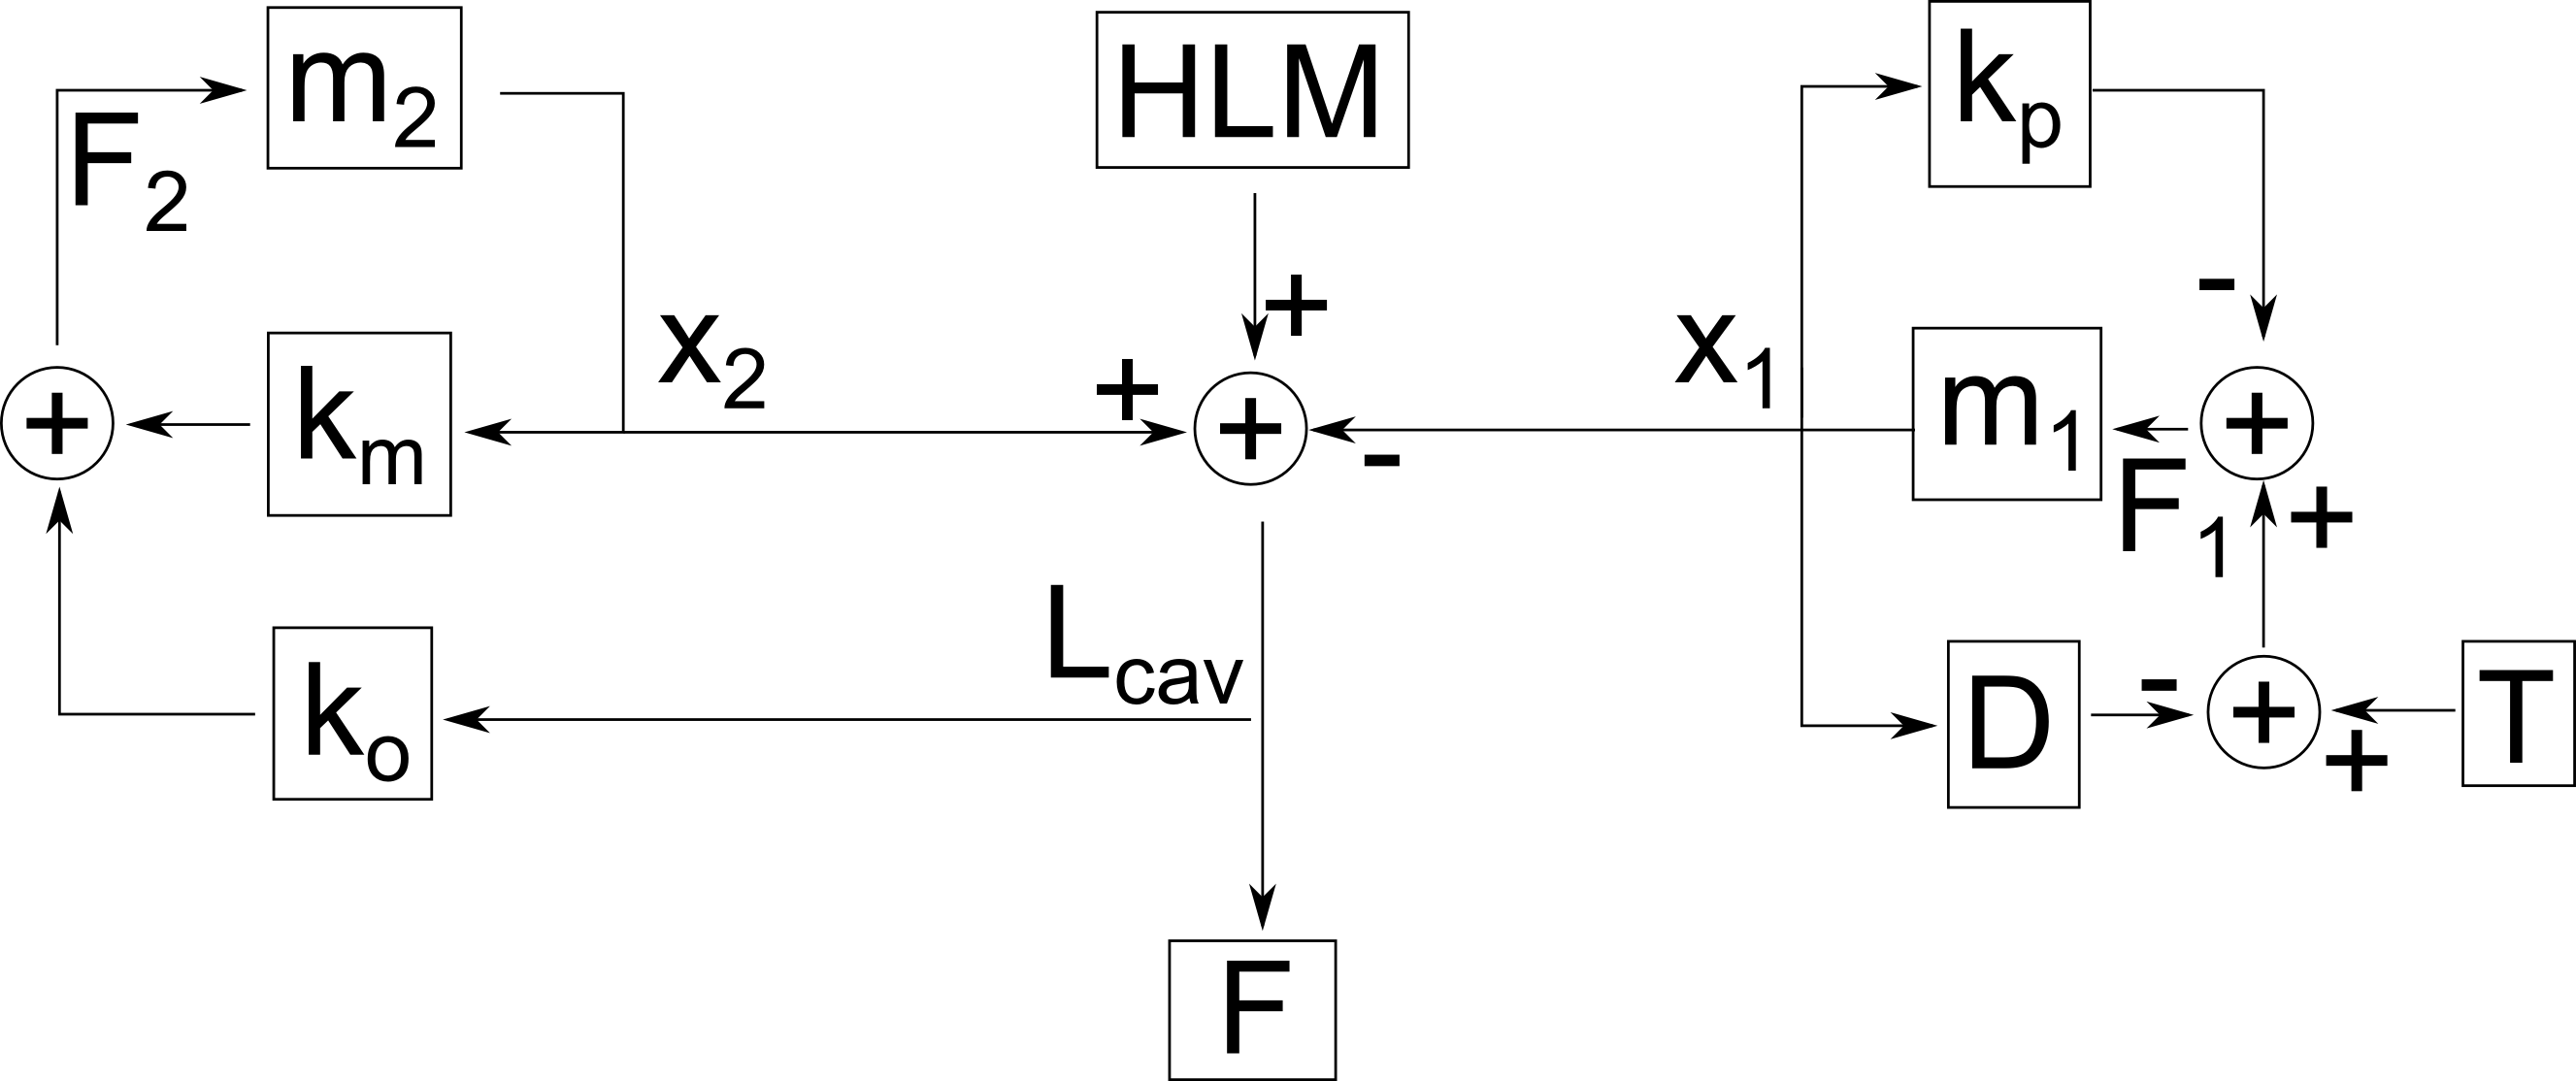
\includegraphics[width=\columnwidth]{figures/controls/blocks2.png}%
%\caption[Block diagram of the cavity with sources of actuation]{Block diagram of the cavity with sources of actuation. Because the optical spring loop is independent of other factors, we can multiply the closed loop gain of the optical spring ($CLG$) by the electronic, mechanical and digital parts of the feedback loop.}%
%\label{fig:cavityloopblocks}%
%\end{figure}

\begin{equation}
\frac{1}{1+OS} = \frac{k_m-m\omega^2}{k_m+k_{os}-m\omega^2}.
\label{eq:OS_CL}
\end{equation}

\subsection{L : Laser PZT}

The laser PZT converts a voltage to a shift in the laser frequency. The number is taken from the product spec sheet.

\begin{equation}
L = -1.7\times 10^6 \mbox{ Hz/V}.
\label{eq:L}
\end{equation}

\subsection{M : Cavity response}

Changes in the laser frequency can be converted into an effective change in the cavity length.  The cavity length $l$ is 0.07 m. This only works for $l\gg\lambda_0$.

\begin{equation}
M=\frac{l\lambda_0}{c}.
\label{eq:loopM}
\end{equation}


\subsection{H : HV amplifier}

H is the HV amplifier (with HV bypass) which drives the laser PZT (See fig. \ref{fig:H}). 
The HV bypass was introduced to bypass the HV amplifier above its unity gain frequency to increase the feedback bandwidth.  
It is described in the SUGWG ALog in entry 412.  
The overall behavior of the amplifier and the bypass is designed to look like this simplified model:
%https://sugwg-alog.phy.syr.edu/aLOG/index.php?callRep=412 data and model in lab2013/FSS/20130908

\begin{equation}
H = \frac{70}{1+\imath f/146}.
\label{eq:Hmodel}
\end{equation}
We actually interpolate the data for this block, so that we don't run into trouble in the discrepancy region.


\begin{figure}[htbp]
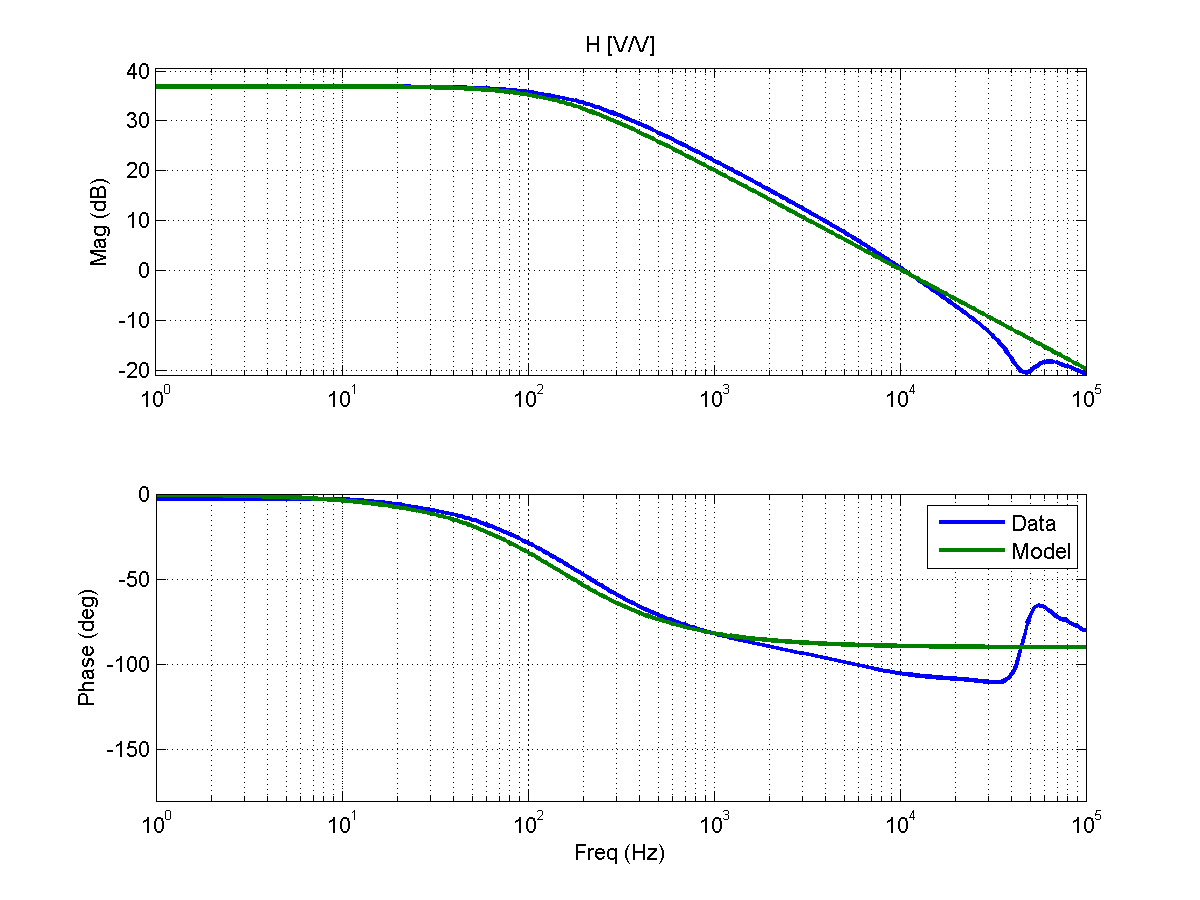
\includegraphics[width=\columnwidth]{figures/controls/H.png}%
\caption{HV amplifier transfer function. Includes a high-frequency bypass to increase feedback bandwidth.}%
\label{fig:H}%
\end{figure}


\subsection{T : Analog PDH feedback to coil drivers}

This is a SR560 that operates between the Trap Servo control signal and the analog drive for the large optic OSEMs.

It is currently set to a 1 kHz 6 dB lowpass with a gain of 200, so it is modeled as 

\begin{equation}
T = \frac{200}{1 - \imath \frac{f}{1\mbox{ kHz}}}.
\label{eq:T}
\end{equation}						



\section{Photothermal effect on loops}
The photothermal effect is directly related to how close the cavity is to resonance. This is affected by the total cavity length and the frequency of the light entering the cavity. In figure \ref{fig:photothermal_blocks}, we see that the photothermal effect (Pt) can be treated as a closed loop acting on the cavity length $L_{cav}$.

\begin{figure}[htp]
\begin{center}
\includegraphics[width=.9\textwidth]{figures/controls/photothermal_blocks}
\end{center}
\caption[Loop diagram for a single degree of freedom]{%
\label{fig:photothermal_blocks}
Loop diagram for a single degree of freedom, including photothermal feedback, Pt. The optical spring loop on the left side ($k_O$, $k_m$, and $m_2$) is affected by the photothermal effect ($Pt$). We measure the behavior of the optical spring by measuring the open loop transfer function of the system at F, then dividing out the transfer functions of the control system ($HLM$, $T$, $D$, etc.). This leaves us with the closed loop transfer function of the optical spring with the photothermal effect. }
\end{figure}


\begin{figure}[htbp]
\centering
\includegraphics[width=343pt]{figures/controls/OLG.png}%
\caption{Open loop TF of the system with several different carrier detunings. Changing the carrier detuning changes the resonant frequency of the springs and their stability. Included are both measurements and corresponding models.}%
\label{fig:OLG}%
\end{figure}
%\Chapter{Photothermal (from paper)}
%\label{ch:photothermal}
%\newcommand{\irm}{\mathrm{i}}

\newcommand{\del}[0]{{}_{{}^\triangle}\!}
\newcommand{\vk}[0]{{\bf k}}
\newcommand{\w}[0]{{\rm w}}
\newcommand{\omg}[0]{{{\Omega}}}
\newcommand{\eq}[1]{equation \ref{#1}}

\section{Introduction}
The Advanced Laser Interferometer Gravitational-Wave Observatory (aLIGO) \cite{Harry2010}, together with its international partners Virgo \cite{2013ASPC..467..151D} and KAGRA \cite{Somiya:2011np}, aim to directly observe gravitational waves emitted by astrophysical sources such as coalescencing of black hole and neutron star binary systems. The installation 
of the Advanced LIGO detectors is completed, and commissioning towards the the first observation run is ongoing. Preliminary astrophysical data is expected in 2015. The sensitivity of those advanced gravitational-wave detectors in the observation band is limited by the quantum noise of light and the thermal noise associated with mirror coatings. A contributor to the thermal noise, expected to dominate in future cryogenic gravitational-wave detectors, is thermo-optic noise \cite{Braginsky2000303, PhysRevD.63.082003, PhysRevD.78.102003}. It is caused by dissipation through thermal diffusion.

The same physics also leads to an intensity noise coupling, known in the literature as photo-thermal effect \cite{Braginsky19991}. The low frequency behaviour of the photo-thermal effect was predicted in \cite{PhysRevD.63.082003} and experimentally measured in a Fabry-Perot cavity by De Rosa et. al. \cite{PhysRevLett.89.237402}. The physics relevant for the the high frequency behaviour, dominated by the details of the coating, was investigated in \cite{PhysRevD.78.102003} in the context of studying thermo-optic noise. It was extended to a full model of the photo-thermal transfer function in \cite{PhysRevD.91.023010}.
Here we explore the thermo-optic effect in the context of an optical spring. The coupling acts as an additional feed-back path. The phase of the coupling becomes important and can directly affect the stability of the optical spring resonance. We can exploit this dependence for a precision measurement of the photo-thermal coupling, even if it is driven by the residual few-ppm absorption of a high-quality optic.

%photo-thermal effect in microresonators \cite{metzgercavity2004}
The desire to lower the quantum noise in the gravitational-wave observation band has driven the power circulating in the Advanced LIGO arm cavities up to about 800~kW. 
%The sensitivity of such detectors is designed to operate at the point where the quantum radiation pressure noise and the shot noise are
%at the same level in the detection band.  This sensitivity limit is commonly known as the standard quantum limit \cite{Caves80, Ni86}.
%Operating at the standard quantum limit requires high laser power, 
The high laser power, in turn, couples the angular suspension modes of the two cavity mirrors. This Sidles-Sigg instability \cite{Sidles06} creates a soft (unstable) and a hard mode, whose frequency increases with the intra-cavity power. The detector's angular control system must control the soft and damp the hard mode, and at the same time must not contaminate the observation band, starting at $10~{\rm Hz}$ in the case of Advanced LIGO. 
Future gravitational wave detectors aim to extend the observational band to even lower frequencies, further aggravating this limitation.
%Perreca et al.
We previously proposed a model \cite{Perreca14}  to overcome the angular instabilities, based on a dual-carrier optical spring scheme demonstrated by Corbitt et al., in 2007 at the LIGO laboratory \cite{Corbitt07}.
%for the length control of a cavity.
%\tcm{for a longitudinal trap of a gram-scale mirror}.
The proposed angular trap setup uses two dual-carrier beams to illuminate two suspended optical cavities which share a single end mirror. %in order to create two longitudinal trap displaced from the center of the gravity of the end mirror.
As first step towards the experimental demonstration of  the scheme we built and operated a prototype, single-cavity optical trap, capable of controlling the cavity length only \cite{LoughThesis}. The data presented in this paper was taken with this prototype.
The next version of the angular trap setup will also allow us to measure the photo-thermal effect on a folding mirror. Heinert et. al. \cite{PhysRevD.90.042001}  predicted excess thermal noise for folding mirrors due to transverse heat diffusion.
The result has not yet been experimentally confirmed, but since the same physics will also lead to an enhanced photo-thermal transfer function, 
the prediction can be verified with a photo-thermal transfer function measurement.

%A single dual beam can trap the end mirror longitudinally.  With the addition of a second dual beam, an additional degree of freedom, e.g. yaw, can be controlled. The experimental demonstration of this model is underway.
%However the proof of the angular trap with a pair of dual beams requires a longitudinal stabilization first.

%In this paper we give an experimental demonstration of the longitudinal trap using a dual-beam injected into a suspended optical cavity with a gram-scale end mirror and we set the requirements to turn off the electronic feedback in order to use the radiation pressure feedback alone. 

%As a  result we obtain the stabilization of the mirror using the radiation pressure and the electronic together. 
%In order to switch completely from the electronic feedback to the radiation feedback system, the mirror suspension should be improved by \tcm{1.314} order of magnitude in the frequency band of interest.

The paper is structured as follows: Sections \ref{sec:DCOS} and \ref{sec:PTE} will review the idea of a dual-carrier optical spring and the photo-thermal effect respectively. 
Section \ref{sec:exp} describes the experimental setup and we discuss the result in section \ref{sec:res}. Finally, section \ref{sec:SCs} suggests a coating modification to make a single-carrier optical spring feasable.
%4 reviews our experimental results.  Section 5 gives our conclusions and lays out the path for the next phase of the project, building an angular trap.}


\section{Dual-carrier optical spring}
\label{sec:DCOS}
A Fabry-Perot cavity detuned from resonance couples the intra-cavity power linearly to the mirror position. The response is delayed by the cavity storage time. The resulting optical spring constant is given by \cite{Perreca14}.
\begin{eqnarray}
\label{eq:KOS1}
K_{OS}^{\rm 1 field} & {\approx} & K_0
\frac{1}{1+\frac{\delta^2}{\gamma^2}-\frac{\Omega^2}{\gamma^2}+i2\frac{\Omega}{\gamma} } \\
K_0 &= & P_0 t_1^2 r_2^2 \frac{8k r_1r_2}{c(1-r_1r_2)^3}\frac{ \frac{\delta}{\gamma}}{(1+\frac{\delta^2}{\gamma^2})} 
\end{eqnarray}
where $P_0$ is the incident power, corrected for mode-matching losses, $k = {2\pi}/{\lambda}$ is the wave vector of the light, $t_i$ and $r_i$ are the mirror amplitude transmissivity and reflectivity for input coupler ($i=1$) and end mirror ($i=2$), and $\gamma$, $\delta$ and $\Omega$ are the cavity line, cavity detuning, and mechanical frequency. The value of $K_{OS}$ lies in either the 2nd or 4th quadrant of the complex plane, and the associated radiation pressure force creates either
a anti-restoring and damping (red detuning) or
a restoring and anti-damping force (blue detuning) \cite{Sheard04}. 

Two spatially overlapping optical fields, the carrier and sub-carrier, with opposite detuning sign and with an opportune power ratio can be used to cancel the instability \cite{Corbitt07}. The total optical spring $K_{OS}$ is the sum of the individual springs
\begin{eqnarray}
\label{eqn:KOSsum2}
K_{OS}=K_{OS}^c+K_{OS}^{sc}
\end{eqnarray}
Where $K_{OS}^c$ and $K_{OS}^{sc}$ are given by equation \ref{eq:KOS1}. The dual-carrier optical spring
can be tuned to lie in the 1st quadrant for the frequency band of interest. When acting on a suspended cavity end mirror with mass $m$ and mechanical suspension spring constant $K_m$ the optical spring becomes a feed-back loop with a closed loop response function
\begin{eqnarray}
\label{eqn:TFloop}
\frac{x}{F_{ext}}=\frac{1}{-m\Omega^2+K_m+K_{OS}}
%\frac{x}{F_{ext}}=\frac{1}{-m\Omega^2+K_m+K_{OS}+K_{\rm extra}}
\end{eqnarray}
The tunability of the optical spring $K_{OS}$ in both magnitude and phase allows experimental fine-tuning of the poles of equation \ref{eqn:TFloop} to lie exactly on the real axis, resulting in an infinite Q of the optical spring (critical stablility).
Experimentally this can be done up to a maximum $Q$, above which the measured transfer function data no longer permits distinguishing between a stable and an unstable spring. The phase of the total spring constant at resonance can then be determined with a precision given by $1/Q$.
The suspension mechanical spring constant has to have a positive imaginary part, but it can be designed to be very small. Loss angles of $10^{-5}$ are easily achievable, and are further diluted by the magnitude of the ratio of $K_{OS}/K_m$. The contribution to the phase of the total spring constant from the mechanical suspension is thus expected to be negligible. The imaginary part of the optical spring $K_{OS}$ on the other hand is closely related to its real part through equations \ref{eqn:KOSsum2} and \ref{eq:KOS1}, and is very accurately predicted based on the resonance frequency, carrier to sub-carrier power ratio as well as the detuning of carrier and subcarrier, i.e. only power ratios and frequencies. As a result, any deviation in phase from the expectation of equation \ref{eq:KOS1} around the optical spring resonance is easily and repeatably observable with a precision given by the inverse of the experimentally resolvable $Q$, and an accuracy determined only by frequency and power ratio measurements.
%highlight relative calibration - based only on frequency measurments and power ratio measurements. This allows for repeatable, reliably measurement of the optical spring parameters, as well as a reliable calibration for measuring any other effects that act as a correction of the effective spring constant near resonance.



%The scheme is based on the optical spring effect that occurs when an optical cavity is detuned from its resonance. The light couples to the mirrors creating either a restoring and anti-damping forces (red detuning) or anti-restoring and damping forces (blue detuning). Two overlapped beams (dual-beam) with opposite detuning sign and with an opportune power ratio will cancel the instability. The use of two pair of beams opportunely off centered will trap the end mirror for its longitudinal and angular degree of freedom.  In this work we focus \tcm{our?} on a single dual-beam scheme to trap the mirror longitudinally \cite{Perreca14}.

%We consider an optical Fabry-Perot cavity with mirror reflectivities of $r_1$ and $r_2$, \tcg{transmisivities $t_1$ and $t_2$}, and a cavity length $L_0$, with the input-mirror mass much larger than the end-mirror mass and with suspension constant spring $k_m$. \tcg{

%The closed-loop frequency response of external force with angular frequency $\Omega$ to end-mirror displacement is

%\begin{eqnarray}
%\label{eqn:TFloop}
%\frac{x}{F_{ext}}=G_{CL}(\Omega)=\frac{1}{-m\Omega^2+k_m+K_{OS}}%=\frac{1}{ms^2+b s+k_m}
%\end{eqnarray}

%where $K_{OS}$ is the sum of the springs of the carrier and subcarrier and frequency detuned at $\delta_c$ and $\delta_{sc}$ respectively:

%\tcg{Where $P_0$ is the power incident on the cavity and $\delta$ is the detuning from cavity resonance in rad/s; these two parameters are specific to the carrier or the subcarrier beam. The wave vector of the light $k = {2\pi}{\lambda}$ and the cavity line width $\gamma = 2 \pi f_p$ are constant.}

%For simplicity below we report the full spring constant as in \cite{Perreca14}
%
%\begin{eqnarray}
%\label{KOS_full_2}
%K_{OS}^{c,sc}=K_0^{c,sc}\left [ \frac{Y^2}{(1-Y^2X)(1-Y^2\overline{X})}  \right ]
%\end{eqnarray}
%
%%is the optical spring constant. %and $\overline{X}$ is the complex conjugate of $X$. 
%where $K_0$ is the 
%%static (frictionless) 
%(mechanical) frequency-independent part of the spring constant:
%
%\begin{eqnarray}
%\label{eqn:K0}
%%K_0=F_0 \cdot 2 i k \cdot (X-\overline{X}),   \quad \mbox{with}\nonumber\\ 
%K_0^{c,sc} = P_0^{c,sc} \cdot 2ik\cdot \frac{2  r_2^2t_1^2}{c} \cdot \frac{X-\overline{X}}{(1-X)(1-\overline{X})}
%%K_0=\eta i \frac{X-\overline{X}}{(1-X)(1-\overline{X})}\quad \mbox{with}\nonumber\\ 
%%\eta=P_0 t_1^2 r_2^2\frac{4 k }{c} 
%\end{eqnarray}
%
%Here $P_0^{c,sc}$ is the input power, $k$ is the wave vector associated with the light field, $t_1$ is the transmissivity coefficient of the input mirror, $X=r_1r_2e^{-2i\delta_{c,sc}\tau}$ is the propagator and  $\overline{X}$ is its complex conjugate, $Y=e^{-i\Omega\tau}$ defines a phase factor, with $\tau=L_0/c$ and $\Omega$ 
%the mechanical frequency of the pendulum.

\section{Photo-thermal effect}
\label{sec:PTE}
Power absorption on the surface of an optic leads to an increase of the surface temperature. The depth of the heated layer is given by the diffusion length $d_{\rm diff}=\sqrt{\kappa/(\rho C \Omega)}$, where $\kappa$, $C$ and $\rho$ are the thermal conductivity, heat capacity and density of the material, and $\Omega$ is the observation angular frequency. In the large-spot size limit, i.e. $\w \gg d_{\rm diff}$, and neglecting coating effects,
% or $\Omega \gg \omg_c$, where $\omg_c=\kappa/(\rho C \w^2)$, 
the displacement of the surface is given by (e.g. \cite{PhysRevD.63.082003,PhysRevD.91.023010})
\begin{equation}
\label{eq:simple}
\del z = \bar{\alpha} \int_0^\infty \!\!\!\!\!\!T dz = \bar{\alpha} \frac{j}{i \omg \rho C}
\end{equation}
where $\bar{\alpha}=2(1+\sigma) \alpha$ is the effective expansion coefficient under the mechanical constraint that the heated spot is part of a much larger optic \cite{PhysRevD.78.102003,PhysRevD.70.082003}. $\alpha$ and  $\sigma$ are the regular linear expansion coefficient and Poisson ratio. $j=P/(\pi \w^2)$ is the absorbed average surface intensity of the Gaussian beam with beam radius $\w$ ($1/e^2$ intensity). This simple picture needs two important refinements. First, for frequencies  $\Omega$ around and below $\omg_c=2 \kappa/(\rho C \w^2)$ the transverse heat diffusion leads to a multiplicative correction factor to \eq{eq:simple}
derived by  Cerdonio et al. \cite{PhysRevD.63.082003}:
\begin{equation}
\label{eq:Cerdonio}
I(\omg/\omg_c) = \frac{1}{\pi} \int\limits_0^\infty du \int\limits_{-\infty}^\infty dv \frac{u^2 e^{-u^2/2}}{(u^2+v^2)\left(1+\frac{(u^2+v^2)}{i \omg/\omg_c} \right) }
\end{equation}
As expected, for $\omg \gg \omg_c$, the correction factor approches 1. 
%which takes a simple form in the transverse Fourier space.
%If this displacement is read out by the same beam profile as the heating intensity (normalized intensity $\hat{I}$), the effective displacement becomes
%\begin{equation}
%\del z_{\rm eff} =  \alpha (1+\sigma) \int d^2 \vk \frac{I_\vk \hat{I}^*_\vk }{i \Omega \rho C+ \kappa \vk^2} =\frac{\alpha (1+\sigma)}{i \Omega \rho C}  \int d^2 \vk W(\vk) \frac{i \frac{\Omega}{\Omega_\vk}  }{1 + i \frac{\Omega}{\Omega_\vk}}
%\label{eq:zeff}
%\end{equation}
%where $\Omega_\vk=\frac{\kappa \vk^2}{\rho C}$, and a weighting function $W(\vk)$ obeying $\int d^2 \vk W(\vk) = I$, the mean intensity, such that we recover equation \ref{eq:simple} in the high frequency limit. Equation \ref{eq:zeff} implies that in general the transfer function from absorbed beam intensity to displacement is given by a weighted sum of poles, where the weighting function is given by the spatial beam profile. For simplicity the derivation given here neglects corrections due to the underlying elasticity problem. This is done in \cite{PhysRevD.63.082003} and results in a slight change in the weighting function $W(\vk)$. 
For a fused Silica substrate, $\rm SiO_2$,  and a Gaussian beam spot radius of $\w=161~\mu{\rm m}$ this correction becomes large below $\omg_c/(2 \pi) = 10~{\rm Hz}$, but is measurably different from unity even at $1~{\rm kHz}$. (See fig \ref{fig:PTcorr})

Second, for high frequencies, the diffusion length becomes comparable to the coating thickness. Since the optical field is reflected by a dielectric stack, the effective mirror displacement is given by \cite{PhysRevD.78.102003,PhysRevD.91.023010}
\begin{equation}
\label{eq:dphic2}
\del z =  \sum_{i}   \left[ \frac{\partial \phi_{\rm c}}{\partial \phi_i} (\beta_i \!+\! \bar{\alpha}_i n_i) 
\!+\!  \bar{\alpha}_i  \right]  \bar{T}_i d_i
\end{equation}
where  $\bar{\alpha}_i$, $\beta_i=dn/dT$ and $n_i$ are the constrained effective expansion coefficient, the temperature dependence of the index of refraction, and the index of refraction itself for layer $i$. $\frac{\partial \phi_{\rm c}}{\partial \phi_i}$, the dependence of the coating reflected phase on the round trip optical phase in layer $i$, is always negative, resulting in a sign change and enhancement of the bracket in \eq{eq:dphic2} for the first few layers. $\bar{T}_i d_i$ is the temperature profile driven by the absorped intensity $j$, integrated across layer $i$. For a $\rm Ta_2O_5\!\!:\!SiO_2$ coating used in gravitational wave detectors we find a measureable enhancement of the photo-thermal transfer function around $1~{\rm kHz}$ \cite{PhysRevD.91.023010}. Additionally, depending on the detailed absorption profile, a sign change can occur above about $100~{\rm kHz}$.

For the experiment parameters discussed in this paper, i.e. a  Gaussian beam spot radius of $\w=161~\mu{\rm m}$ and a mirror coating with about 13 doublet layers both effects are relevant in the $100~{\rm Hz}$ to $1~{\rm kHz}$ band. Their contributions are plotted in figure \ref{fig:PTcorr}.

\begin{figure}[htp]
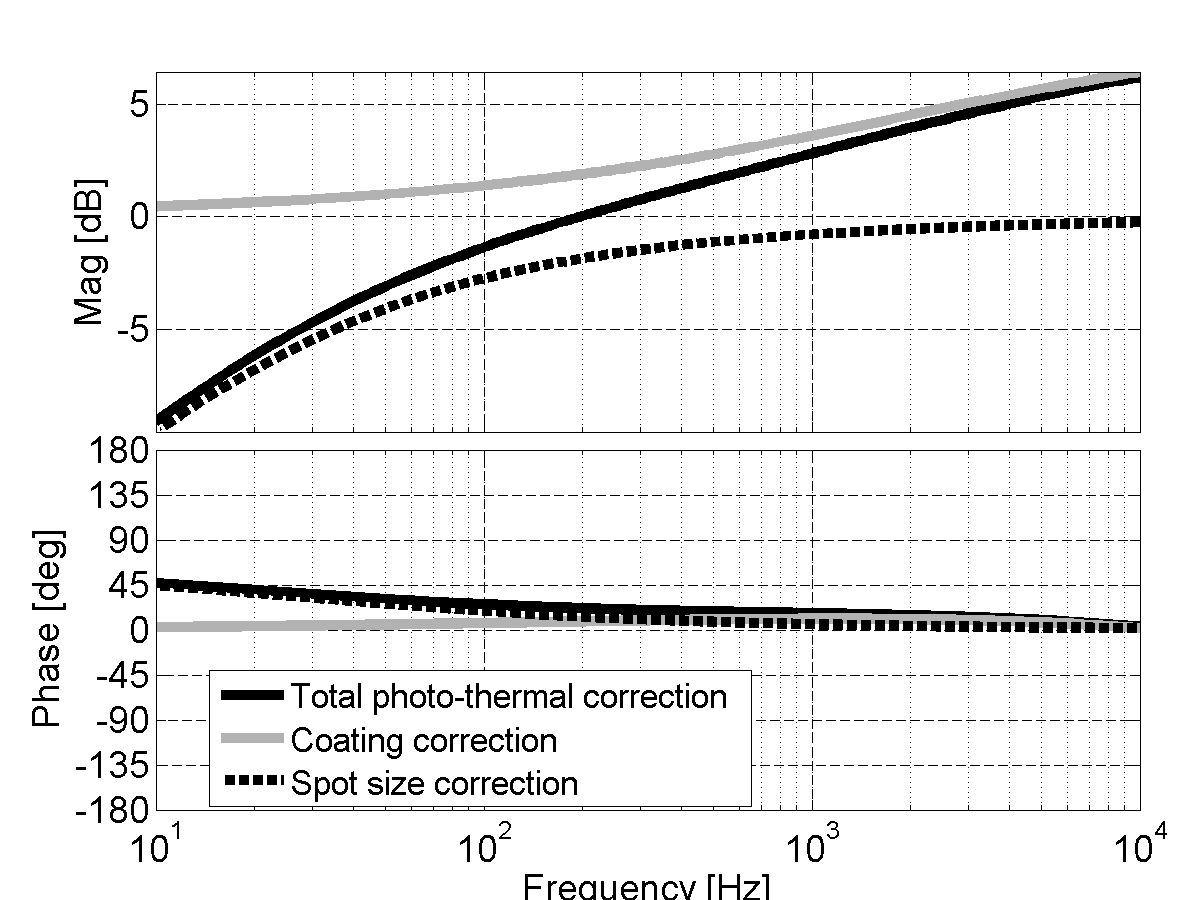
\includegraphics[width=\columnwidth]{figures/photothermal/FigOT1.png}%
\caption[Coating corrections]{Correction factors for the photo-thermal transfer function of a fused silica mirror with a dielectric coating (solid black). The solid grey trace is the coating correction for a 13-doublet $\lambda/4$  coating. The dashed black trace shows the effect of a Gaussian beam spot with $\w=161~\mu{\rm m}$ radius. To get the full transfer function, multiply with \eq{eq:simple}, adding an overall $1/f$ shape.
The calculation is based on material parameters show in table \ref{SiO2}. }%
\label{fig:PTcorr}%
\end{figure}

\section{Experimental setup}
\label{sec:exp}

\subsection{Cavity}

%\begin{table}[h]
%\scriptsize
%\begin{tabular}{|l|l|l|l|l|l|l|}
%\hline
%$\lambda_0$ & Mirror RoC & $L_0$    & Spot size  & FSR      & Finesse & Cavity Pole \\ \hline
%1064 nm     & 5.0 cm     & 7.0 cm & 161 $\mu$m & 2.14 GHz & 7500    & 143 KHz     \\ \hline
%\end{tabular}
%%\end{table}
%%
%%\begin{table}[h]
%\begin{tabular}{|l|l|l|l|}
%\hline
%$\delta f_{C}$ & $\delta f_{SC}$ & $P_{C}$    & $P_{SC}$ \\ \hline
%213-290 KHz    & 27-36 KHz     & 225-239 mW & 65-78 mW \\ \hline
%\end{tabular}
%\end{table}

\begin{table}[htp]
\begin{tabular}{|l|l|}
\hline
$\lambda_0$ & 1064 nm \\ \hline
Mirror RoC & 5.0 cm \\ \hline
$L_0$ & 7.0 cm \\ \hline
Spot size  & 161 $\mu$m\\ \hline
FSR      & 2.14 GHz \\ \hline
Finesse & 7500 \\ \hline
Cavity Pole & 143 KHz\\ \hline
\end{tabular}
%\end{table}
%
%\begin{table}[h]
\begin{tabular}{|l|l|}
\hline
$\delta f_{C}$ & 213-290 KHz \\ \hline
$\delta f_{SC}$ & 27-36 KHz \\ \hline
$P_{C}$ input& 225-239 mW \\ \hline
$P_{SC}$ input & 65-78 mW \\ \hline
\end{tabular}
\caption[Parameters of the optical spring cavity]{Parameters of the optical spring cavity. The range of values for the carrier and sub-carrier detuning frequency ($\delta f_{C}$, $\delta f_{SC}$) and input power ($P_{C}$, $P_{SC}$) indicate the variation between individual measurements.}
\label{tab:longCavParams}
\end{table}


The optical spring cavity is composed of two suspended mirrors in a vacuum chamber, each with radius of curvature RoC = 5$\,$cm and power transmissivity $T = 4.18\times10^{-4}$.
The measured finesse is $7500\pm 250$ and the cavity length is $L_0 = 7.0\pm0.2\,$cm. We chose a short cavity to minimize frequency noise coupling. The cavity has a free spectral range (FSR) of about 2.14$\,$GHz and cavity pole $f_{pole} = \gamma/(2 \pi) = 143~{\rm kHz}$. 
The input mirror mass is $300\,$g, designed to be heavy to make it insensitive to radiation pressure; it is suspended as a single stage pendulum with mechanical resonances, i.e. position, pitch and yaw, close to $1\,$Hz. The end mirror has a mass of $0.41\pm 0.01~{\rm g}$ and is $7.75~{\rm mm}$ in diameter. It is suspended with three glass fibers from a $300~{\rm g}$ steel ring, shown in figure \ref{fig:smallmirrorpic}. The steel ring has diameter of $7.6~{\rm cm}$ and is itself suspended.
% and damped by local active feedback.
%described in Sec.$\,$\ref{sec:glasssus}. 
%The glass fiber resonances are about 18 Hz. 
The input mirror is actively controlled by an electronic feedback system, while the end mirror is 
free to move in the glass suspension abobe its resonance frequency of $18~{\rm Hz}$, and is only subject to the optical spring radiation pressure. 
%The end mirror motion is locked to the input mirror using optical springs and laser feedback.

\begin{figure}[htp]
\includegraphics[width=.8\columnwidth]{figures/photothermal/smallmirrorpic.png}%
\caption[End mirror picture]{A picture of the small end mirror suspended from a steel ring by glass fibers. The ring is suspended from a small optics suspension (SOS) with tungsten wire.
The SOS provides DC alignment control while allowing the mirror to move freely above the 18Hz resonance of the fiber suspension. The end of the fiber is a small glass nub attached to the mirror with epoxy. This produces a fairly high suspension Q of about $5 \cdot 10^5$. The resulting contribution of damping in the opto-mechanical spring is insignificant compared to the damping from the optical field.}%
\label{fig:smallmirrorpic}%
\end{figure}

%\subsection{Glass suspension for the end-mirror}
%\label{sec:glasssus}

%The 0.4 g end mirror is 7.75 mm in diameter. It is suspended by glass fibers from a 300 gram steel ring which is 7.6~cm in diameter as shown in figures \ref{fig:smallmirrorpic} and \ref{fig:smallmass}. The steel ring is damped by local active feedback. The mirror is suspended using thin glass fibers tensioned to a 18 Hz resonance frequency, suppressing ring-to-optic motion coupling above 18 Hz. 

%The glass fibers are attached to the end-mirror using vacuum-safe epoxy. The connection points are small cone-shaped glass nubs at the mirror end of the fibers. These nubs are constructed by cold welding the tip of a glass rod to a small mirror blank. The cold weld method is useful becasue it creates a weak joint that breaks cleanly. The fibers are pulled from the nubs, and then the nubs are broken off of the mirror. We are left with a monolithic fiber attached on one end to the pulling rod, which can be mounted in the steel ring, and on the other end to a nub, which has a radius of curvature fitted to the end mirror.  We epoxy these nubs to the end mirror, creating robust, low-loss connections that do not damage the mirror coating. The resulting suspension has a high Q factor ($Q = 5 \times 10^5$). This procedure was adopted because several attempts at welding directly to the mirror resulted in damaged coatings.

%\begin{figure}[htb]
%	\centering
%		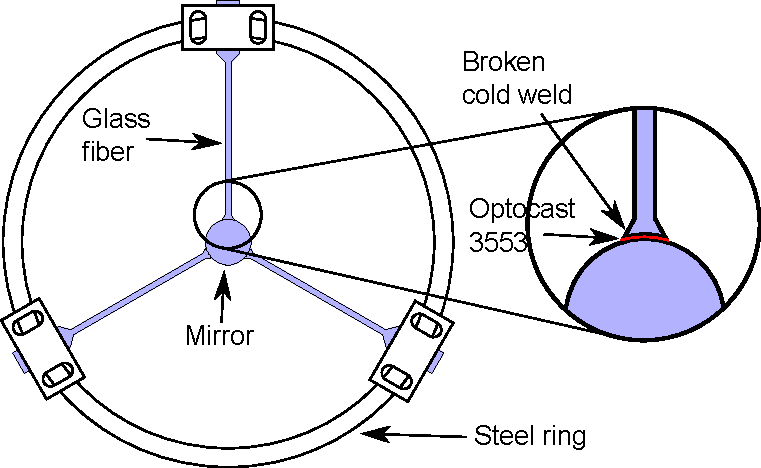
\includegraphics[width=0.8\columnwidth]{figures/smallmass2.pdf}
%	\caption{The configuration of the small mass suspension. The end mirror is glued to fibers which are clamped in a steel ring.}
%	\label{fig:smallmass}
%\end{figure}

\subsection{Input field preparation}
\label{sec:layout}

%The experimental setup is shown in figure \ref{fig:layout}. 
The optical field incident on the optical spring cavity consists of two beams, a carrier and a subcarrier, as described in Section \ref{sec:DCOS}.
As shown in figure \ref{fig:layout}, a 1064 nm laser is split into a carrier and a subcarrier beam at the polarizing beam splitter PBS1. 
In the subcarrier path two acoustic optic modulators (AOMs) are used to impose a relative frequency shift $\Delta$, 
on the subcarrier beam, leaving it at a set detuning from the carrier beam.  
$\Delta$ is set using an external signal generator (see Sec.\,\ref{sec:subservo}).
The two beams recombine at PBS2 and proceed towards the Fabry-Perot cavity with opposite polarization.
The total power and the power ratio between the carrier and subcarrier beams are set by two half wave-plates $\lambda /2$. 

The subcarrier beam is modulated by a 35 MHz electro-optic modulator (EOM). We measure the modulated light reflected by the cavity with a resonant radio-frequency photodiode (RFPD) and then demodulate to read out the cavity length with the Pound-Drever-Hall technique (PDH) \cite{Black01}.  We use the subcarrier to derive a PDH singal because the subcarrier requires less detuning than the carrier. We can use the PDH signal to actuate on the laser and the suspensions to lock the cavity, then turn down the gain and use the PDH signal for readout. 

A small offset added to the PDH error signal shifts the locking point of the cavity to the side of the resonance, setting the subcarrier detuning $\delta_{sc}$. 
We choose to introduce an offset that corresponds to a negative frequency (``red'') detuning. Consequently the carrier is positively (``blue'') detuned at  
$\delta_c = \Delta + \delta_{sc}$. An electronic locking servo can be used to process the error signal and feed back to coils, actuating on
magnets mounted on the large cavity mirror, and to the laser frequency.
%the control signal at the laser in order to have a stable controlled system.

\begin{figure}[htb]%
\centering
\includegraphics[width=\columnwidth]{figures/photothermal/layout3}%
\caption[A schematic layout of the optical trap experiment]{A schematic layout of the optical trap experiment. The light from the laser is split into the carrier and subcarrier paths at PBS1, with a ratio determined by the $\lambda/2$ plate. The subcarrier path is frequency shifted by two AOMs under the control of the subcarrier servo (described in detail in Section \ref{sec:subservo}), then recombined with the carrier at PBS2. The co-aligned mode-matched beams enter the cavity, then are individually monitored at the output. We can use the 35 MHz EOM and RFPD in a PDH scheme to read out the cavity length or lock the cavity.}
\label{fig:layout}
\end{figure}


\subsection{Subcarrier Servo}
\label{sec:subservo}

The high FSR of our cavity (2.14 GHz) meant that available AOMs, with much lower operating frequency ranges (65 to 95$\,$MHz), were not suitable to lock the carrier and subcarrier on adjacent resonances.  
However, this same operating range prevents a single AOM from locking the two beams on the same resonance, due to the small cavity linewidth.
%
%we must operate with the two beams (carrier and subcarrier) detuned around the same resonance
%as the minimum drive frequency is higher than the linewidth, while 
%the maximum is less than the \ac{fsr}.
%
Thus, we set the subcarrier on the same resonance fringe as the carrier using two AOMs, each one shifting the laser frequency by about 80MHz in opposite directions.
One is driven by an $80~{\rm MHz}$ crystal oscillator, while the other is driven by a servo-locked Voltage controlled oscillator (VCO) running slightly offset from $80~{\rm MHz}$ (see figure \ref{fig:layout}).
%, which gives us the
%knob to detune the subcarrier relative to the carrier.
%{Figure \ref{fig:layout} shows the basic layout of the subcarrier servo loop.
To control the offset frequency the $80~{\rm MHz}$ signal from the crystal oscillator is mixed with the VCO output, producing a signal at the frequency difference. This difference signal is then mixed with the drive from a function generator, creating the error signal for the servo.  The servo drives the frequency modulation input of the VCO, closing the loop and locking the subcarrier beam to a fixed frequency offset from the carrier beam.

%\tcg{We produce a beat signal between the two oscillators and we lock the beat signal to a function generator which is set at our desired frequency offset. 
%Thus we can set the carrier-to-subcarrier offset frequency directly using the knob on the function generator.} \ \tcm{Not clear to me.} \tcm{We may need a pic of the electronic setup}
This setup significantly suppresses the frequency noise from the VCO. The remaining subcarrier frequency noise (relative to the carrier) is dominated by fluctuations in the path length difference between carrier and sub-carrier, see figure \ref{fig:layout}.

%due to RF signal path length differences in the drive cables to the two AOMs.

%, since we are subtracting the coherent frequency noise from the first AOM with the second AOM. 
%Using a low frequency (sub-MHz) function generator to lock to the difference between the drives is also beneficial because tunable oscillators generally have a frequency noise that is proportional to the set frequency.




%\begin{figure}[htb]
%\centering
%		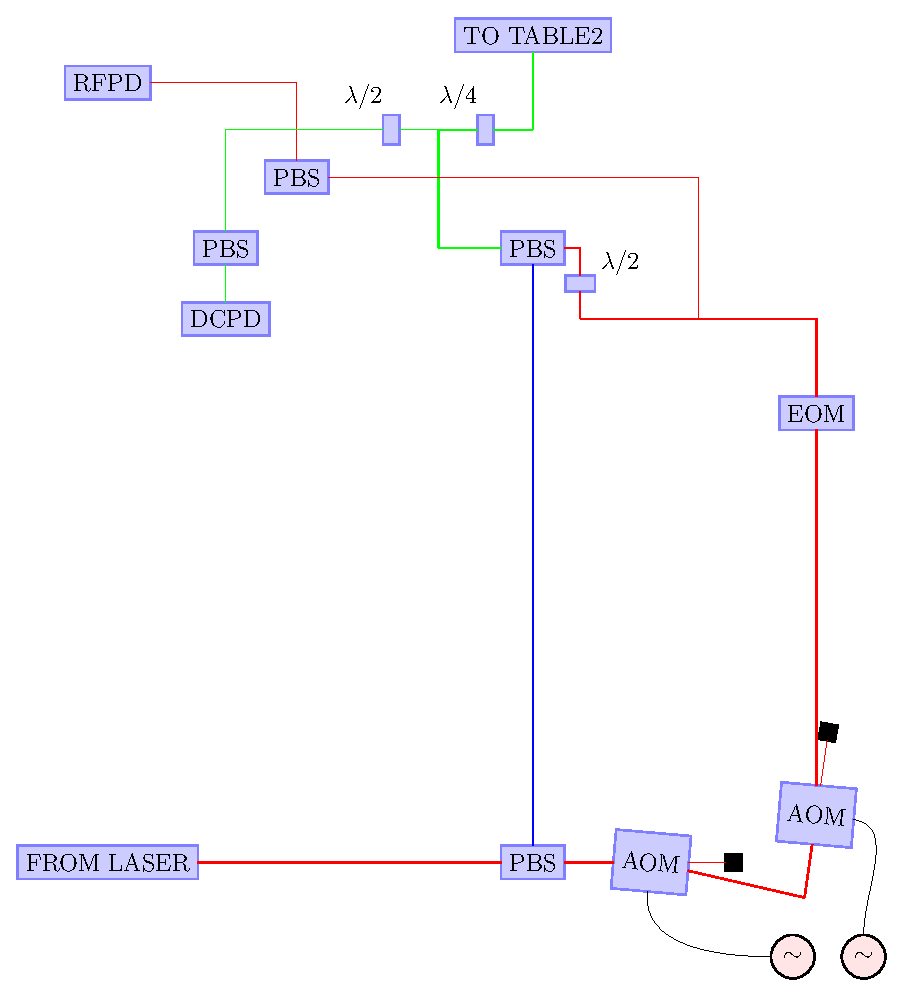
\includegraphics[width=0.5\columnwidth]{figures/scservo}
%	\caption{This is our layout for generating orthogonally polarized
%        carrier and subcarrier beams. \tcb{Having this AND fig. \ref{fig:layout} seems redundant.}}
%	\label{fig:scservo}
%\end{figure}


%\subsection{Parameter space}
%The stability of the system described in equation \ref{eqn:TFloop} depends on the detuning of both the carrier and the subcarrier beams and the input power ratio. We can determine the stability for our system, a suspended cavity with a light end mirror and a relatively heavy input mirror, by considering the phase margin of the loop. In figure \ref{fig:paramspace} we show the phase margin of the open loop gain of the system at the optical spring resonance; a system with a positive phase margin will be stable while one with a negative phase margin will not.
%
%Figure \ref{fig:paramspace} only shows two of the four optical spring parameters: the carrier detuning and the subcarrier detuning. The input carrier power and the input subcarrier power were left unchanged. However, changing the carrier  subcarrier detuning also slightly affected the cavity alignment, resulting in small changes in the coupling efficiencies, and therefore in the intracavity power, independent of the expected effect of detuning the cavity.
%For figure \ref{fig:paramspace} the carrier power and the subcarrier power were thus fitted to quadratic functions of the carrier and subcarrier detuning, to account for this experimentally observed dependence of the transmitted powers.  
%%with finesse of $\sim 7500$, length $L_0 = 7\,$cm with mechanical resonances, i.e. pitch and yaw, close to $1\,$Hz  for the input mass and $\sim 19\,$Hz for the end mass. The weight of the input mass is close to 300 g while the end mirror is $\sim 0.5\,$g. 
%The detuned frequencies of carrier and subcarrier and the input power ratio determine the regions of the parameters space where we expect stability of the cavity system, i.e. the mirror being trapped longitudinally.  
%
%
%\begin{figure}[htb]
  %\centering
  %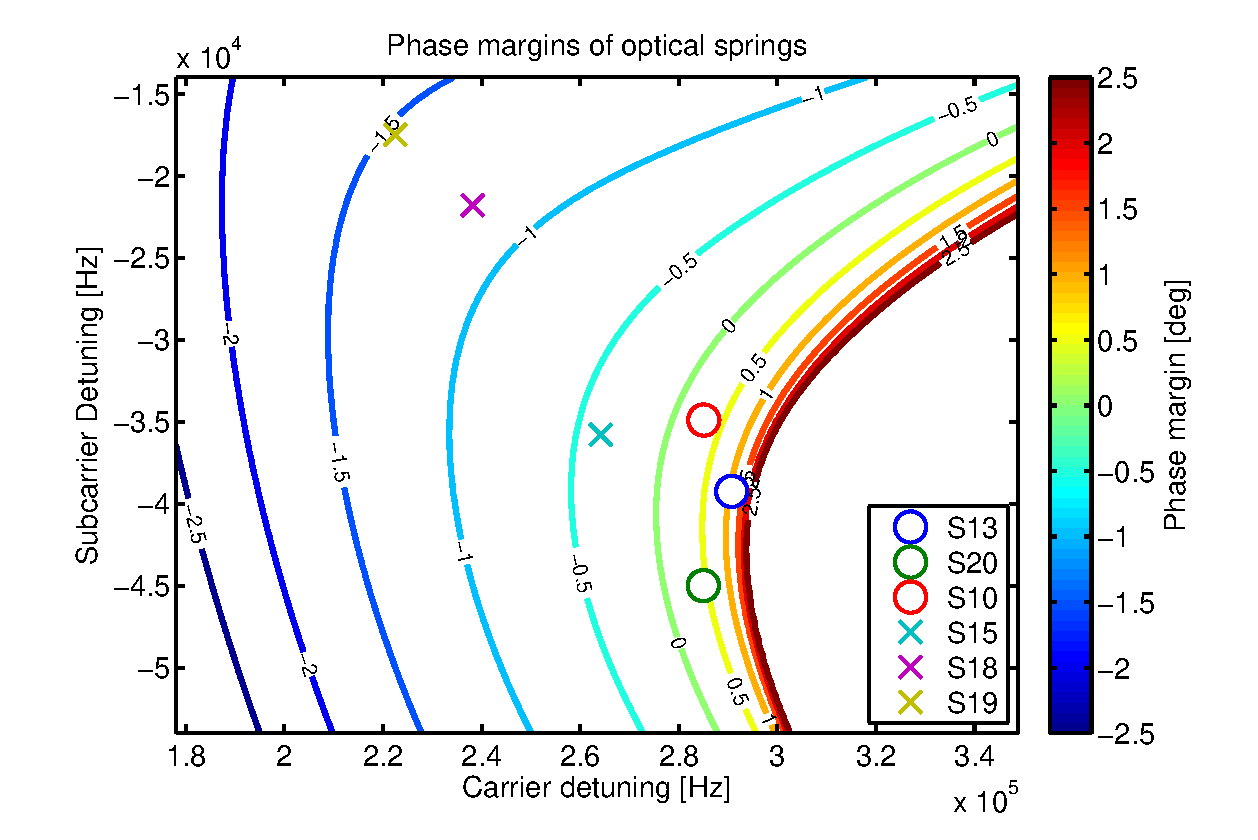
\includegraphics[width=\columnwidth]{figures/param_space2a}
  %\caption{Phase margin (degrees above -180) in the carrier vs subcarrier detuning parameter space. A stable system, denoted in the plot with circle, will have a positive phase margin. For each point in the parameter space, the power parameters are chosen from a fit to the measured spring data.
  %%\tcm{Must be changed...totally}The parameter space of possible optical traps. 
    %%While keeping the frequency difference between carrier and subcarrier
    %%constant, we can scan the subcarrier detuning.
    %%The colored contours show the resonant frequency of the optical trap.
    %%Also shown are lines of constant phase margin, which indicate the
    %%stability of the system.
    %%\tcb{This plot should be updated to either eliminate the stars and make
    %%a general parameter space plot or use stars corresponding to the data
    %%taken.
    %%It is not immediately obvious how we could do that with the data from the
    %%second run due to the number of dimensions that seem to vary across
    %%measurements.
    %%Maybe axes of C-SC frequency offset and power(which impacts both the
    %%subcarrier offset and power ratio).}
    %}
  %\label{fig:paramspace}
%\end{figure}
%% figure from Dropbox\BallmerLab\plots\opticalSpringFit\plot_data7.m



%Results:
%  - we took data and fit it to both full and naive models
%  - we got error bars
%  - within the error bars, both models kinda make sense.


\section{Results}
\label{sec:res}

\begin{figure*}[thb]%
\centering
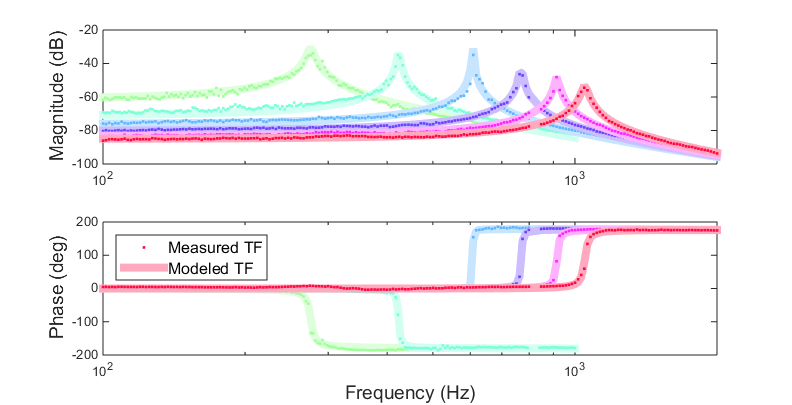
\includegraphics[width=.7\paperwidth]{figures/photothermal/newOSfit.png}%
\caption[Stable and unstable optical springs]{Data and modeled transfer function for a series of stable and unstable springs. The modeled transfer functions include the full coating and spot size correction, computed with the measured average absorption. Stable springs show a phase drop of 180 degrees at resonance, while unstable springs show a rise of 180 degrees.}%
\label{fig:springs}%
\end{figure*}
%\tcm{MUST BE REWRITTEN IN A POSITIVE WAY. WE have nice results to show not only problems. Because the previous version was literally depressing
%I remove it. Jim this is a section that you should have in your thesis, so you can plug it in and we will see how it flows.}
%\tcm{We also need to to say what function we are plotting...equation 1? 2? }

%At the beginning of the experiment, our goals were to measure and then accurately model a series of stable and unstable optical springs. During the course of the measurements, we saw a consistent trend towards instability; each measurement we took was more unstable than our model predicted it should be. We realized that this behavior was exactly what we would see from the photo-thermal effect. We made a new goal of measuring the effects of the photo-thermal absorption.

Using the setup described in the previous section, we locked the cavity using a PDH error signal from the sub-carrier, feeding back to the laser frequency actuator and, at low frequencies, the heavy input coupler position. In this configuration we fine-tuned the optical spring parameters (carrier and sub-carrier offset and power) and 
measured the PDH control loop open loop transfer function. Dividing out the known PDH loop sensing and actuation function gives us the closed loop transfer functions of the optical springs (figure \ref{fig:springs}). While we demonstrated stable and unstable dual-carrier optical springs, these measurements revealed a significantly smaller phase margin of the optical spring than expected based on equation \ref{eqn:TFloop}, suggesting the presence of a non-radiation-pressure feed-back path.

At a few ppm, the absorption $A$ of the mirrors has a very small effect on the cavity finesse and no significant impact on the total transmitted power. However, this small amount of absorption still causes local heating of the optic, driving fluctuations in the surface position of the optic, and thus the cavity length, via the photo-thermal effect. If this is the dominant effect, we should be able to include the photo-thermal effect in our model and fit the model to the data, using the absorption as the free parameter. Given a set of optical spring measurements done under similar conditions, we would then expect to find a consistent absorption coefficient across measurements.

%\begin{table*}[t]
%\small
%\begin{tabular}{| l || c | c | c | c | c | c | c |}
%\hline 
%Run & 14 & 10 & 9 & 16 & 17 & 18 & 19 \\
	%\hline
	%\hline
%$f_{res}$ [Hz]& $386 \pm 3$& $423 \pm 2$& $432 \pm 2$& $609 \pm 5$& $772 \pm 6$& $919 \pm 7$& $1054 \pm 8$\\
%$P_{tc}$ [mW]& $44.1 \pm 0.9$& $45.3 \pm 0.9$& $45.3 \pm 0.9$& $49.3 \pm 1.0$& $54.0 \pm 1.1$& $59.8 \pm 1.2$& $67.2 \pm 1.3$\\
%$P_{ts}$ [mW]& $63.9 \pm 1.3$& $73.2 \pm 1.5$& $73.2 \pm 1.5$& $62.6 \pm 1.3$& $62.1 \pm 1.2$& $62.3 \pm 1.2$& $61.8 \pm 1.2$\\
%$df$ [KHz]& $320 \pm 5$& $320 \pm 5$& $320 \pm 5$& $300 \pm 5$& $280 \pm 5$& $260 \pm 5$& $240 \pm 5$\\
%\hline$P_{ic}$ [mW]& $225 \pm 16$& $239 \pm 17$& $239 \pm 17$& $227 \pm 17$& $225 \pm 17$& $225 \pm 17$& $223 \pm 17$\\
%$P_{is}$ [mW]& $69.5 \pm 1.6$& $78.3 \pm 1.7$& $78.2 \pm 1.6$& $67.6 \pm 1.6$& $66.5 \pm 1.6$& $66.2 \pm 1.5$& $65.6 \pm 1.6$\\
%$\delta f_c$ [KHz]& $284 \pm 8$& $290 \pm 7$& $290 \pm 7$& $267 \pm 8$& $250 \pm 8$& $233 \pm 8$& $213 \pm 9$\\
%$\delta f_s$ [KHz]& $-36 \pm 5$& $-30 \pm 4$& $-30 \pm 4$& $-33 \pm 6$& $-30 \pm 6$& $-27 \pm 6$& $-27 \pm 7$\\
%\hline$A$ [ppm]& $2.9 \pm 2.16$& $2.7 \pm 2.20$& $2.9 \pm 1.80$& $2.8 \pm 1.77$& $2.5 \pm 1.31$& $2.5 \pm 1.08$& $2.7 \pm 0.96$\\
%$\phi$ [mRad]& $-15 \pm 11$& $-15 \pm 12$& $-17 \pm 10$& $-25 \pm 15$& $-29 \pm 15$& $-36 \pm 15$& $-46 \pm 16$\\
%
%
%\hline
%
%
%\end{tabular}	
%\normalsize
%\caption{Measured values [$f_{res}$, $P_{tc}$, $P_{ts}$, $df$], translated to optical spring parameters [$P_{ic}$, $P_{is}$, $\delta f_c$, $\delta f_s$] and the calculated absorption coefficient $A$. \tcb{sort by fres}}
	%\label{tab:springs}
	%
%\end{table*}

\subsection{Analysis}

For each measured optical spring transfer function we record the carrier and subcarrier transmitted powers, $P_{tc}$ and $P_{ts}$, the optical spring resonance frequency $f_{res}$, and the difference between the carrier and subcarrier detunings $df_c-df_s$, which is set by the function generator frequency.   

%Using these values we can accurately determine the parameters [$P_{is}$,$P_{ic}$, $df_c$,$df_s$], namely
%the power coupling into the cavity and the detuning for both the carrier and the subcarrier at the time of measurement. %\tcr{This is useful because we had a little bit of alignment drift during the course of the experiment.}
%Equation \ref{eqn:TFloop} allows us to convert these four parameters into an optical spring transfer function.

We can then fit the data $d$ using a model $m$, which includes the photo-thermal effect. In particular we fit the ratio $d/m$ using a least-squares fit to minimize $E$, the error.
\begin{equation}
E=\Sigma \left|\frac{d}{m}-1\right|^2 
\end{equation}

We fit for a small magnitude offset, the subcarrier detuning $df_s$, and the absorption $A$. We assess the fitting errors by modeling the noise in each frequency bin of the transfer function measurement, and propagating this noise through the fit. Four of the optical spring transfer functions  had a measurement noise of a little less than $1~{\rm dB}$, while the optical springs at $276~{\rm Hz}$ and $422~{\rm Hz}$ had a significantly higher noise of about $3~{\rm dB}$. We think this noise is dominated by intra-cavity power fluctuations, most likely due to angular fluctuations.

The remaining parameters (cavity transmitted powers and carrier-sub-carrier frequency spacing) we treat as systematic errors. We propagated their measurment errors through the fit. We used a $2\%$ measurement error for the power measurements and  a $1~{\rm kHz}$ error for the frequency separation.




%\begin{eqnarray}
%E=\Sigma w|d-m|^2 \hspace{5pt} w = m^{-2}\\
%\frac{\partial E}{\partial p_i} = 0\\
%\Sigma w(d-m) \frac{\partial m}{\partial p_i} = 0
%\label{eq:dEdP}
%\end{eqnarray}
%We are evaluating two different models: 
	%(i) a naive model, with a simple $1/f$ behavior representative of a single slab of fused silica (equation \ref{eq:simple}), and
  %(ii) a combined model, adding both coating and diffusion effects to the naive model (equations \ref{eq:Cerdonio} and \ref{eq:dphic2}).

%We can calculate the error for each fitted parameter based on the noise in the transfer function and the discrepancy between the best fit model and the data. 

%We determine the change in the model $m$ with respect to the six parameters of the system (three measured and three fitted)
%\begin{equation}
%M_i' = \frac{\partial m}{\partial p_i}
%\label{eq:}
%\end{equation}

%We construct a vector $\epsilon$ to contian the error on each of the six parameters. Then we assert that the noise $n$ seen during the data recording were likely caused by the fluctation of some or all of the parameters. We combine that with the mismatch between model and data to arrive at the uncertainty in the different parameters.

%\begin{eqnarray}
%M'\epsilon = (n+d-m);\\
%M'^\dagger M'\epsilon = M^\dagger(n+d-m);\\
%\epsilon = (M'^\dagger M')^{-1}M^\dagger(n+d-m);
%\label{eq:epsilonDef}
%\end{eqnarray}
%\begin{equation}
%\epsilon = (M'^\dagger M')^{-1}M^\dagger(n+d-m);
%\label{eq:epsilon}
%\end{equation}

%This gives us the uncertainty in absorption $e_{A}$ due to the fluctuations of other parameters during measurements.


%$M'$ is an $a\times b$ matrix where a is the number of frequency points in the transfer function and b is the number of parameters used in total: three fixed parameters and three fitted parameters. We determine $M'$ by taking the partial derivative of the model $M$ at each frequency point with respect to each parameter $p_i$. $M'^\dagger$ is the transposed complex conjugate of $M'$.

%We calculate the error in the absorption $A$ by propagating the individual measurement errors through the analysis, refitting the absorption $A$, and adding all errors in quadrature. Errors for $P_{ts}$ and $P_{tc}$ are $2\%$ of the measured value, accounting for oscilloscope inaccuracies, fluctuations over the course of the measurement, and DC offsets of the photodiodes.  Error for the frequency offset are a flat 5KHz; we have determined that the frequency output is accurate to 1 or 2 KHz, but we did not always place the dial precisely during measurements. $f_{res}$ can be determined to about 1 Hz, limited by how well we can fit the data given the finite frequency spacing. It is this error on the resonance frequency that dominates the total measurement error.

After determining the absorption $A$ for each optical spring transfer function measurement, we can take a statistical-error-weighted average to arrive at the most probable absorption coefficient for the mirror.  For the full photo-thermal model we measure a consistent absorption of  $2.60\pm0.08$ ppm ($\pm 0.06$ ppm statistical,  $\pm 0.05$ ppm systematic) (see figure \ref{fig:abs}). The naive $1/f$ model yields an absorption of $3.27\pm0.10$ ppm ($\pm 0.08$ ppm statistical,  $\pm 0.06$ ppm systematic).  The detailed model with coating and spot size corrections is slightly preferred by the data over the naive $1/f$ model, i.e. the result is more consistent with the same absorption at all frequencies. However the errors in our mesurement are too large to make this statement with any sigificant certainty.

%\begin{eqnarray}
%A_ = \frac{\Sigma\left(A\epsilon_{A}^{-2}\right)}{\Sigma\left(\epsilon_{A}^{-2}\right)}
%\hspace{20pt}
%\sigma_{ABS} = \sqrt{\frac{1}{\Sigma\left(\epsilon_{Ai}^{-2}\right)}};
%\label{eq:weighting}
%\end{eqnarray}


Since this measurement is based on the missing optical spring phase on resonance, we can also express the result as extra phase. Near the resonance the optical spring constant is close to real, while the photo-thermal effect is almost purely imaginary. Thus we approximately find for the extra phase $\phi$
\begin{equation}
\phi =  2 m \Omega^2 \frac{c}{2} \frac{\bar{\alpha}}{\Omega \rho C \w^2 \pi} A I_{\rm corr}
\approx 0.4^{\circ} \frac{A I_{\rm corr}}{1~{\rm ppm}} \frac{f}{1~{\rm kHz}} 
\label{eq:phase}
\end{equation}
Here the leading factor of two accounts for the two mirrors, $I_{\rm corr}$ is the real part of the total correction factor plotted in figure \ref{fig:PTcorr}, and we used the material parameters for fused silica (see table \ref{SiO2}).  
Figure \ref{fig:phi} shows the measured extra phase on resonance, together with the prediction from the photo-thermal feed-back with the best-fit absorption. The figure also shows the expected phase due to the dual-carrier optical spring, as well as the total phase of the complete model. Finally it is worth mentioning that this is a remarkably precise way to measure the phase of the open loop transfer function - the  error bars in figure \ref{fig:phi} are as small as $0.04^{\circ}$.






%
%Since the main effect of the thermo-optic feed-back is a change in the optical spring phase margin, we can alternatively express our measurment as additional phase required to fit the data. 
%{\tcr{rewritten till here}}
%We can use this value to create a model for $\phi_{pt}$ as a function of $f_{res}$ by varying $df_c$.  We can then compare this model to the measured $\phi_{pt}$.
%
%We can see in Figure \ref{fig:phi} that there is excellent agreement between the full model and the measured loss angles $\phi_{pt}$.  
%
%From this point, we calculate the quality factor $Q$ and total (photothermal effect and optical spring damping) loss angle $\phi_{pt+os}$ for each model ($Q = \frac{f_{res}}{\mbox{FWHM}} = \frac{1}{\phi_{pt+os}}$).  Using the fitted model rather than data is a much more accurate method of determining the optical spring $Q$ because the measured data is limited in frequency resolution, making it difficult to determine the full-width-half-max (FWHM) accurately.  Using the models that fit the data closely, we can increase the resolution and get a reliable measure of the Q  (and thus $\phi_{pt+os}$).
%
%We can similarly calculate the loss $\phi_{os}$ for an optical spring with the same parameters but no absorption (and thus no photo-thermal effect).  Because the effect is purely imaginary and the real part of the transfer function is consistent, the phases can be subtracted. We arrive at $\phi_{pt} = \phi_{pt+os} - \phi_{os}$, the loss due to the photo-thermal effect (see figure \ref{fig:phi}).  
%
%
%%For each one of these errors, we add or subtract the error from the measured value in one of the parameters, then recompute $\phi_{pt}$ and $A$. We find the difference between upper and lower propagated errors for each parameter, add them in quadrature, and finally divide by 2 to get the error bars for $\phi_{pt}$ and $A$.
%
%Once we have calculated $A$ for a number of measurements, we can take an error-weighted average to arrive at the most probable absorption coefficient for the mirror.  We can use this value to create a model for $\phi_{pt}$ as a function of $f_{res}$ by varying $df_c$.  We can then compare this model to the measured $\phi_{pt}$.
%
%We can see in Figure \ref{fig:phi} that there is excellent agreement between the full model and the measured loss angles $\phi_{pt}$.  We measure a consistent absorption of about  $2.7 \pm 0.06$ ppm (see figure \ref{fig:abs}). The calculated reduced chi-squared is about 0.32, indicating that our statistical error is much smaller than the systematic error. The agreement between the data and the naive model is worse, yielding a reduced chi-squared of about 4.6 for an absorption of about $6.49 \pm 0.21$ ppm.

\begin{figure}[htb]%
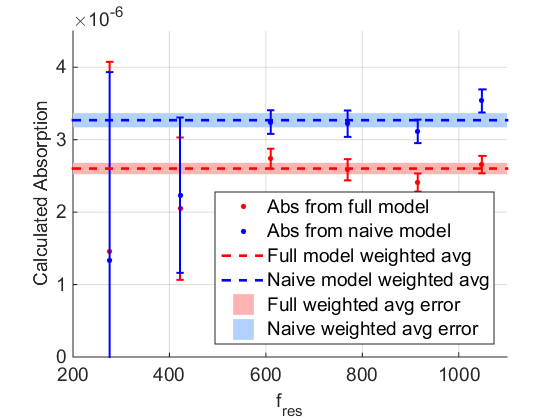
\includegraphics[width=\columnwidth]{figures/photothermal/newABS.png}%
\caption[Absorption fit for naive and full models]{Absorption fit for naive and full models. The full model absorption is consistent with a constant absorption of  $2.60\pm0.08$ ppm. The naive $1/f$ model predicts $3.27\pm0.10$ ppm. The transfer function data for the lowest two resonant frequencies was significantly noisier. Also, at lower frequencies the photo-thermal  effect has a smaller effect on the total optical spring. Both effects result in the larger error bars at low frequencies.}
\label{fig:abs}%
\end{figure}

\begin{figure}[htb]%
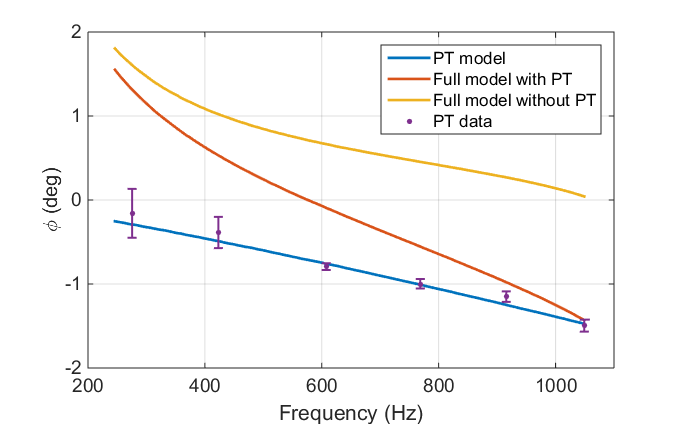
\includegraphics[width=\columnwidth]{figures/photothermal/newPhi.png}%
\caption[Feedback phase in the system]{Feedback phase in the system due to the optical spring and photo-thermal effect. The measured extra phase is consistent with $2.60$ ppm of absorption. The error bars are as small as $\pm 0.04^{\circ}$, a remarkable precision for an open loop transfer function phase measurement.
}
\label{fig:phi}%
\end{figure}

%\begin{figure}[htb]%
%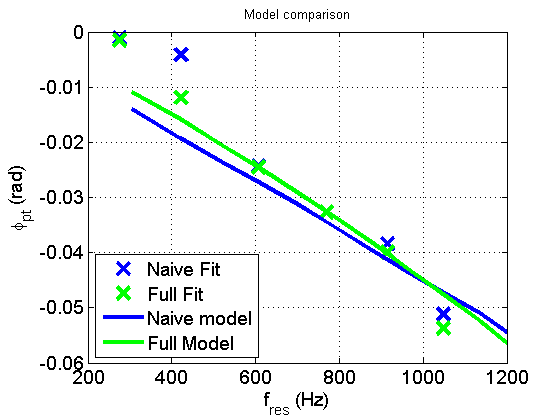
\includegraphics[width=\columnwidth]{figures/phi.png}%
%\caption{Data and model for the loss angle $\phi$ for the full model.}%
%\label{fig:phi}%
%\end{figure}



%We can use the fact that the phase of the optical spring is very closely tied to its stability to measure the absorption $A$ of the mirrors very accurately. As the optical spring system approaches instability, its quality factor (Q) rapidly increases. By measuring the Q of the optical spring and comparing to the model which does not include the photo-thermal effect, we can determine the phase of the actuation function and thus the absorption of the optic to high accuracy (see Figure \ref{fig:absvsq}).  We note that optical springs closer to the stability critical point (resonant frequency of about 500 Hz in our measurements) have a large (positive or negative) slope 
%
%The six measurements given in table \ref{tab:springs} are shown in figure \ref{fig:springs}. These are measurements of the locked trap cavity open loop transfer function. In this case we drive the locked servo, which in turn actuates on the laser PZT and input mirror position, in high and low frequency ranges, respectively. We measure the signal immediately before the servo. From figure \ref{fig:springs}, we can identify that three of the configurations are stable (with phase dropping 180 degrees at the resonant frequency) and three are unstable (with phase rising 180 degrees instead).
%
%
%\begin{figure}[ht]
%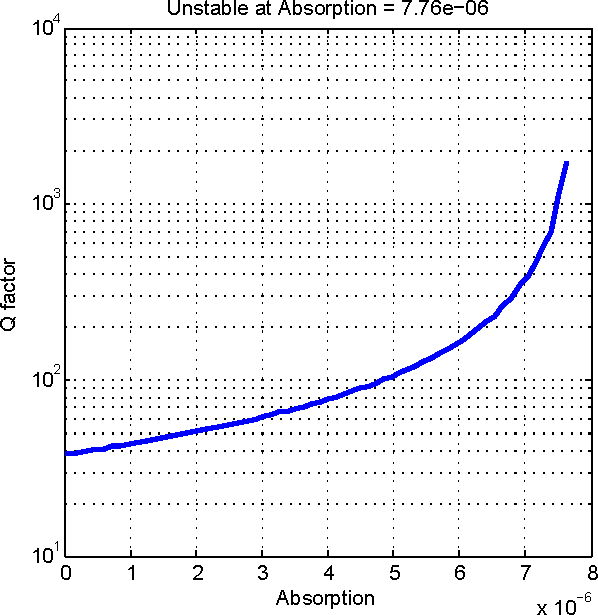
\includegraphics[width=.8\columnwidth]{figures/AbsVsQ.png}%
%\caption{Model for optical spring Q as a function of absorption. Given a set of input parameters for an optical spring, the Q will be directly related to the absorption coefficient.  Optical springs that are closer to the stability critical point have a higher absolute slope, which means that we can measure the absorption more precisely.}%
%\label{fig:absvsq}%
%\end{figure}
%
%\newpage
%
%\begin{figure}[ht]
%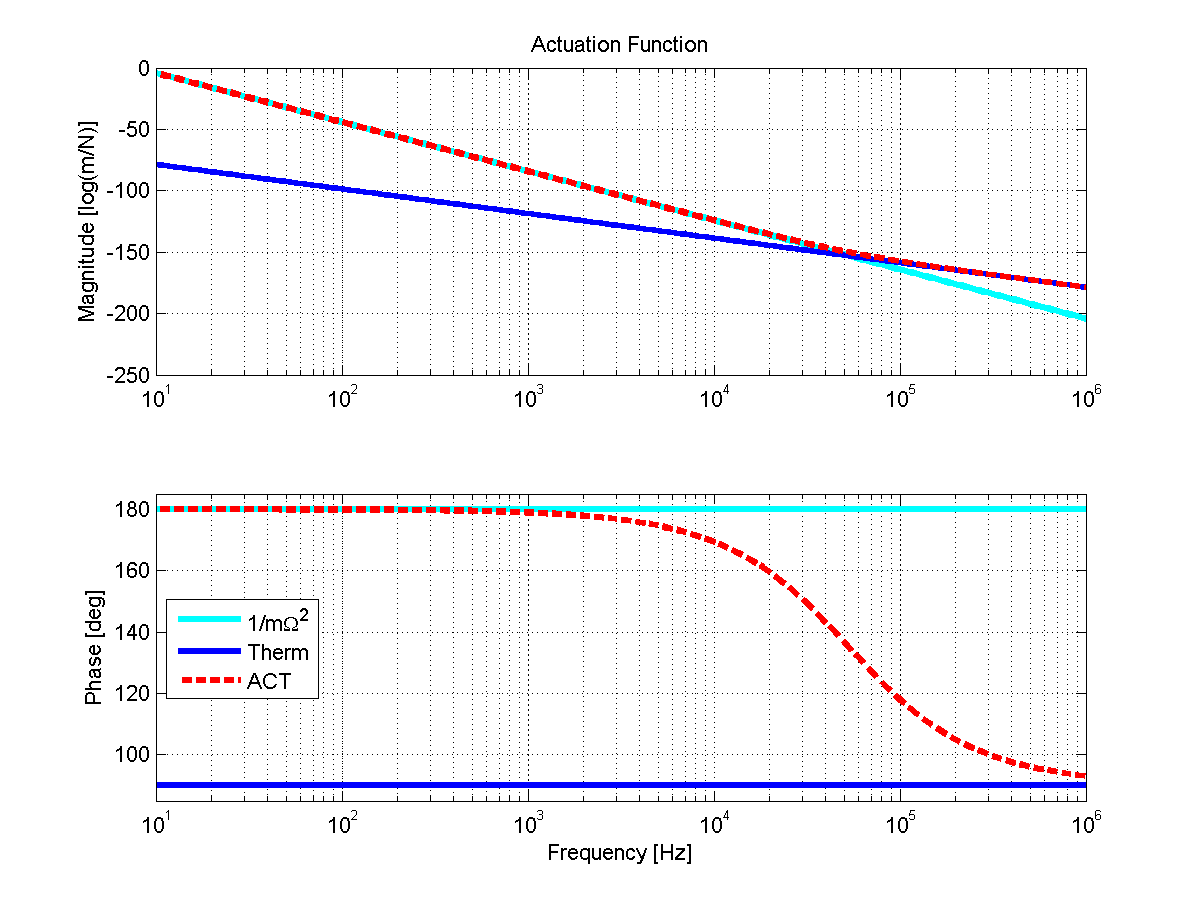
\includegraphics[width=.8\columnwidth]{figures/ACT.png}%
%\caption{Actuation function for small mass. As the frequency increases, the phase contribution from the photo-thermal effect becomes significant.\tcb{should go in intro}}%
%\label{fig:act}%
%\end{figure}
%
%
%Using this method, we can measure the absorption of the mirrors to be $6 \pm x$ ppm \tcm{need to verify this number}, which is \tcb{more accurate/as accurate/cooler} than previous measurements.

%A frequency-dependent thermal expansion of the optic can accurately reproduce the stability behavior observed \cite{BallmerThesis}. This effect is due to absorption of intra-cavity light (about 5 ppm) on the surface of the optic which causes local heating following the thermal diffusion law:
%
%\begin{equation}
%C \rho \frac{\partial T}{\partial t} = \kappa \nabla^2 T
%\label{eq:fourier}
%\end{equation}
%
%Where $C$ is the heat capacity, $\rho$ is the density, and $\kappa$ is the thermal diffusivity.  The heated areas expand at a rate governed by thermal expansion coefficient $\alpha$; because this heating is local, the only possible direction of expanion is the optical axis, towards the center of the cavity. This introduces a factor of $\eta$, Poisson's ratio.
%
%
%\begin{equation}
%\delta z = \alpha(1+\eta) \int_0^\infty{T dz}
%\label{eq:deltaz}
%\end{equation}
%
%The low frequency behavior of this effect is easy to understand and model.  However, when the cavity length is fluctuating, there is frequency dependent behavior that is interesting.
%
%\begin{eqnarray}
%\frac{\delta z}{F_{ext}} = \imath\frac{c}{2 C \rho} \frac{1+\eta}{\pi w^2} \frac{2 \alpha A}{\Omega}\\
%\frac{\delta z}{\delta L} = -m\Omega^2\imath\frac{c}{2 C \rho} \frac{1+\eta}{\pi w^2} \frac{2 \alpha A}{\Omega}
%\label{eq:}
%\end{eqnarray}




%We found a range of stable and unstable springs and we can model the behavior well (see figure \ref{fig:springs}). The largest uncertainty in the measurement was the intra-cavity power.  This is affected by mode matching, cavity alignment, cavity finesse, and input power. As we mentioned earlier, we were very careful to maintain the coatings of the mirror during the cavity construction process.  \tcb{We do have a question about whether the cavity finesse is affected by mode matching.}  We know the input power and the power fluctuation from the laser data sheet \tcb{(and we can predict how much intensity noise the Subcarrier Servo introduces)}. This leaves one big question: the cavity alignment. Because of our digital system design, we do not have any feedback at very low frequencies, instead relying on the pendulum behavior of the suspension.  This can cause trouble with drifting, which we expect is the single largest contributor to variances in the intra-cavity power.
%
%Intensity fluctuations also couple to cavity length via heating of the surface of the mirrors. It's a lot weaker than other noise sources at low frequencies, but only drops as $1/f$, compared to $1/f^2$ for most other noise sources. With this coupling (on both mirrors) and an assumed absorption of 5 ppm, the data can be fairly well explained\cite{BallmerThesis}.



%From our model, we can estimate the length of the stability region of a particular optical trap based on the detuning and power parameters. For the parameters \tcb{$\delta_{C} = 285 \mbox{KHz}$, $\delta_S = -35\mbox{KHz}$, and $P_C/P_S = 3.50$} we find a stable region of \tcb{27 \mbox{pm}}. Thus, if we can lower our RMS length noise to about \tcb{14 pm} we could feasibly turn off or significantly reduce active feedback.
%
%Figure \ref{fig:trapnoise} shows the various noise sources in our experiment. \tcb{Once we get the final plot, we should describe interesting things in it.} At high frequency, our current limitation is the laser frequency noise.  At lower frequencies, we have laser intensity noise and seismic motion to contend with.

%It looks like the intensity noise contribution is much higher than it is plotted on the graph.
%
%The behavior of the intensity noise at 500 Hz could use some explaining. Is this because we are dividing by the closed loop tf?
%
%What do we have in terms of optical trap for this measurement?
%
%Subcarrier: -50KHz, Carrier: 280KHz, Transmitted power ratio C/SC 0.720
%\tcb{We need the updated plot!}
%\tcb{Using this noise measurement, we can see that by doing X, Y, and maybe Z, we could feasibly run the trap with NO active feedback to the cavity length.}

%\begin{figure}[htb]
%\centering
  %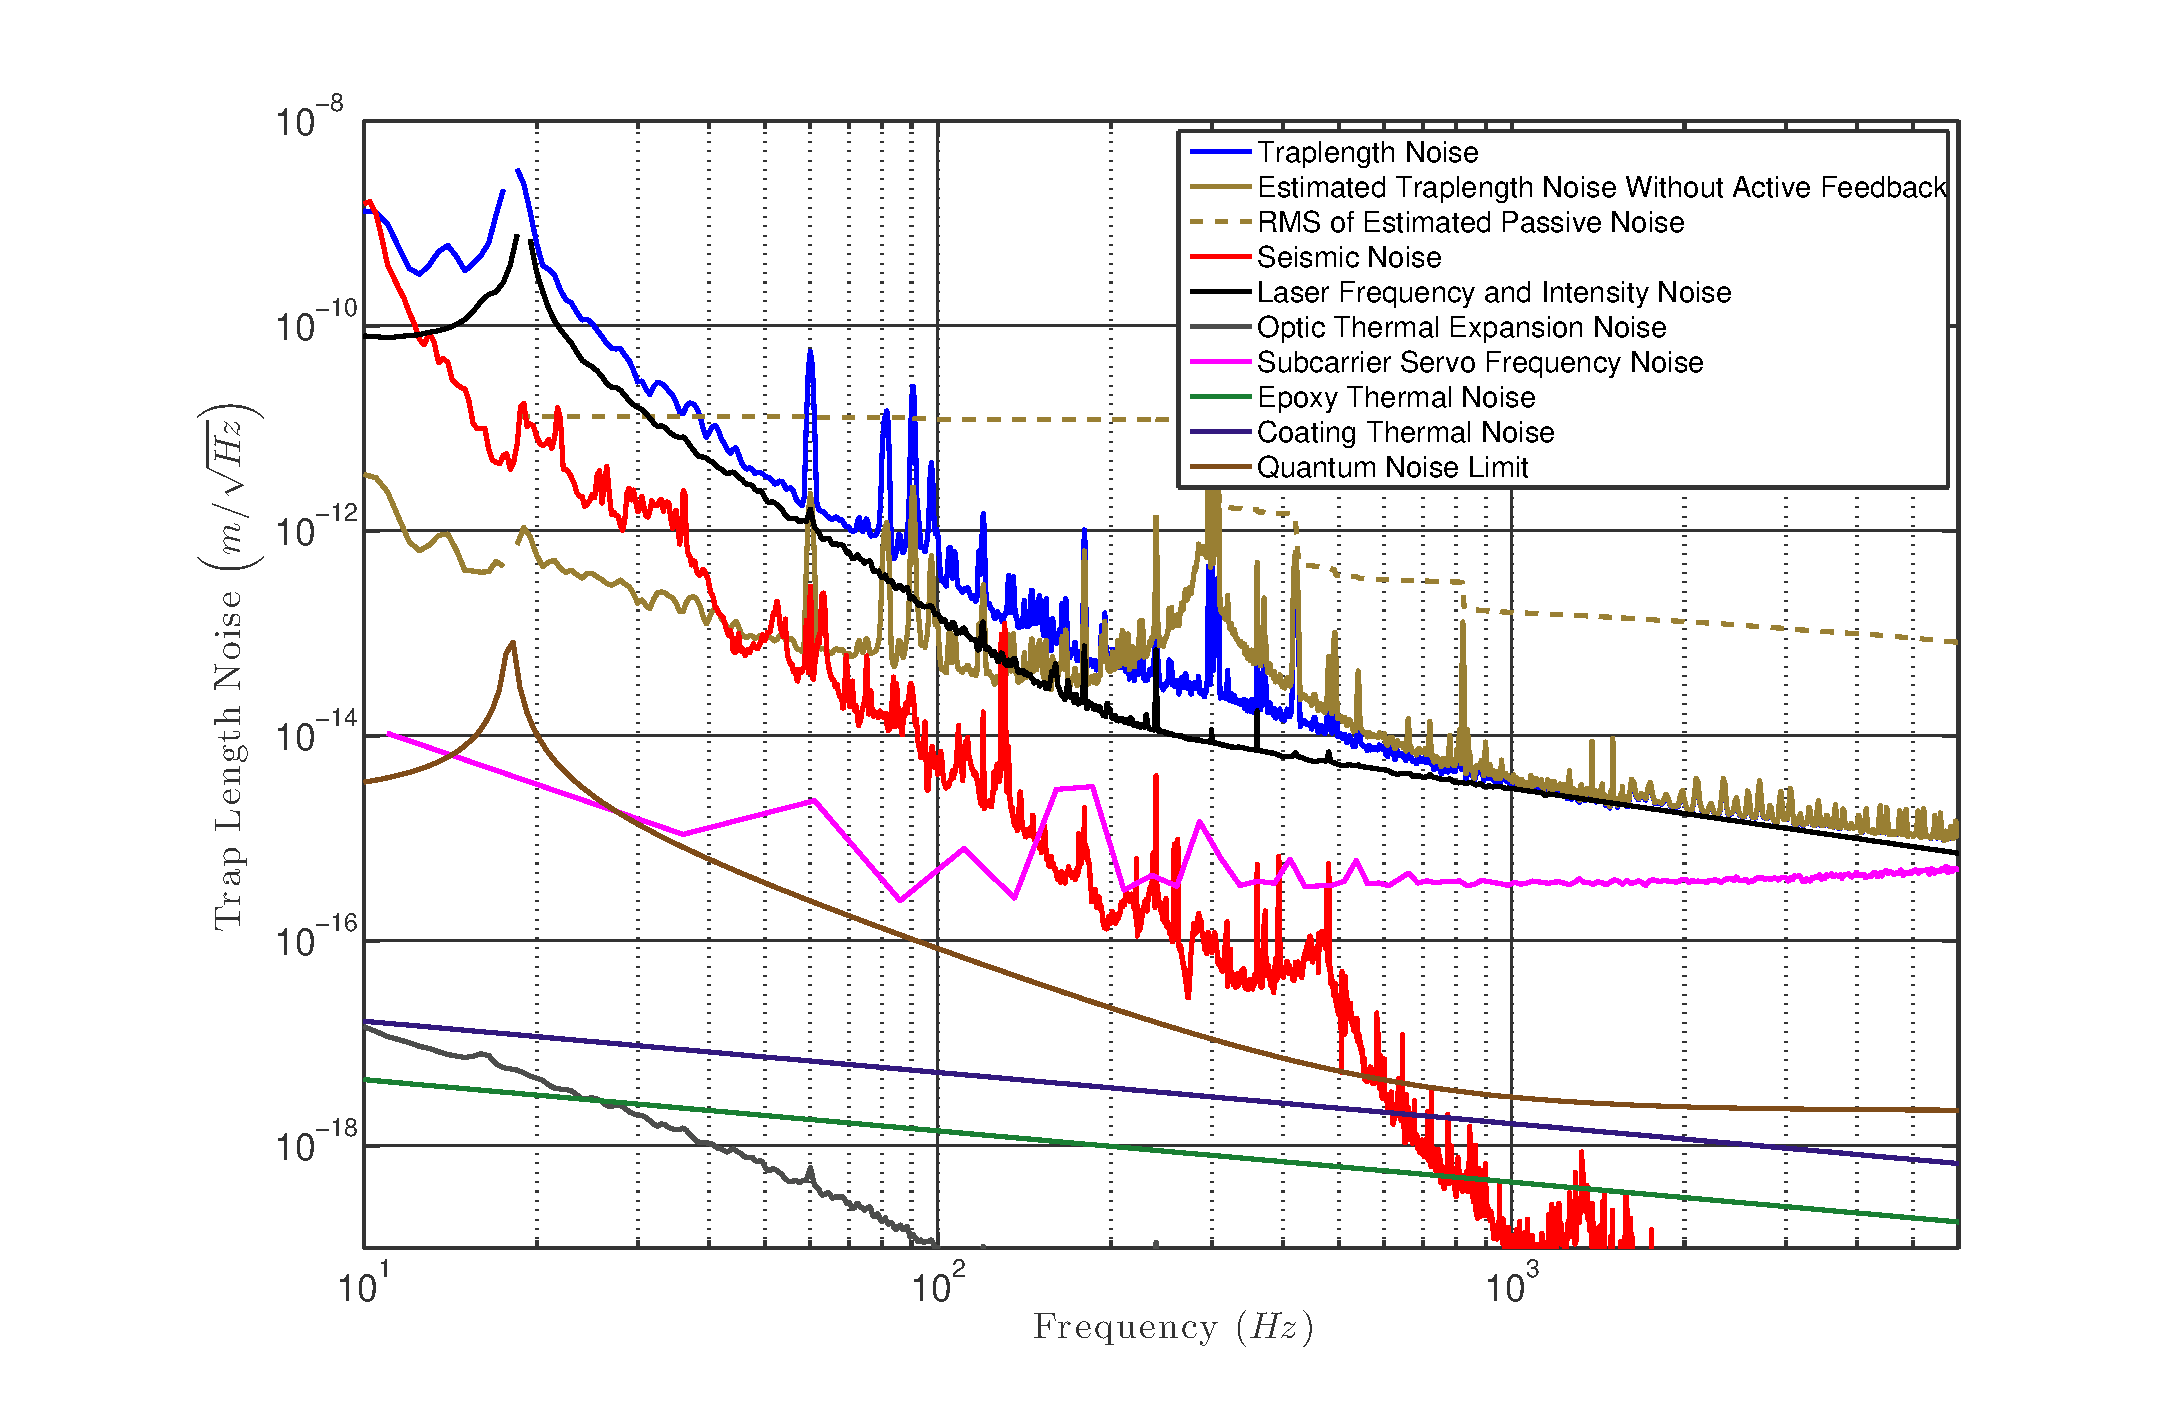
\includegraphics[width=0.8\columnwidth]{figures/trapnoise}
  %\caption{This is the noise budget for the experiment. SC: -50 C: 280
    %TPR .720.
    %\tcb{Updated plot (14.08.02). We may want to have a separate plot
    %for the estimated noise without active feedback.}
    %}
  %\label{fig:trapnoise}
%\end{figure}

\section{Stable single-carrier optical spring}
\label{sec:SCs}
In the experiment at hand the photo-thermal feed-back always pushed the optical spring resonance closer to instability.
Perhaps the most interesting question is whether we can change the sign of this feed-back path and exploit it to stabilize an otherwise unstable optical spring. It was pointed out in \cite{PhysRevD.91.023010} that this naturally occurs above about $100~{\rm kHz}$ for a regular dielectric coating. 
At those frequencies the thermal diffusion length only affects the first few layers of the coating, which affect the overall coating reflected phase differently than the rest of the coating.
However it is actually quite simple to get this sign inversion to occur at a much lower frequency. Increasing the thickness of the inital half-wavelength $SiO_2$ layer - but keeping it an odd multiple of half the wavelength - will boost the effect from the first layer, thus lowering the frequency at which this sign inversion occurs. Indeed this effect can be strong enough that the damping effect from the sub-carrier is not needed to generate a stable optical spring. To illustrate this, figure \ref{fig:SCsprings} shows a set of six optical springs with parameters identical to the ones shown in figure \ref{fig:springs}, except that we set the sub-carrier power to zero (i.e. they are single-carrier optical springs), and we increased the first $SiO_2$ coating layer from $0.5$ wavelength to $20.5$ wavelength.

Such a modified coating would thus allow detuned self-locking  of an optical cavity, using just one laser frequency. It does rely on a small amount (order 1 ppm) of optical absorption in the coating, but this level of absorption is often unavoidable anyway, and does not prevent high-finesse cavities. 
\begin{figure*}[thb]
\centering
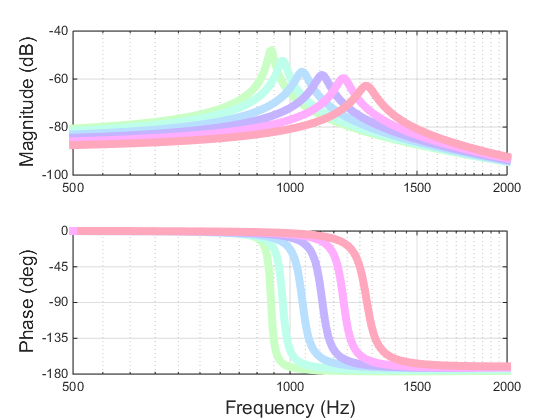
\includegraphics[width=.7\paperwidth]{figures/photothermal/singleCarrierSprings}
\caption[Stable single-carrier optical springs]{Stable single-carrier optical springs (no sub-carrier) with modified coating - the first coating layer is $20.5$ wavelength thick. See text for details. The six traces otherwise have the same parameters as the best-fit optical springs in figure \ref{fig:springs}. }
\label{fig:SCsprings}
\end{figure*}








\section{Conclusions}
We observed photo-thermal feedback in an experimental optical spring setup for a 0.4 gram mirror. We made measurements for a range of optical spring resonant frequencies, and used a least squares fit to calculate the absorption. The data is consistent with the predictions of the complete model presented in Section \ref{sec:PTE}, but only sligthly prefers it over a simple model that ignores any heat diffusion in the coating and transverse to the optical axis. We also show that a small modification of the first layer of the high-reflectivity coating would be enough to reverse the sign of the photo-thermal feed-back, to the extent that a single-carrier, dynamically and statically stable optical spring becomes feasable.

%We presented a model for a complete photo-thermal effect in a cavity optical springs. This model included radial diffusion behavior, coating expansion, and bulk expansion. We described the optical trap experiment at Syracuse University as it relates to the creation of optical springs influenced by the photo-thermal effect. We measured stable and unstable optical springs, which showed more instability than the basic optical spring model predicted. We used a naive model and a complete model of the photo-thermal effect to fit the data. We found excellent agreement between the measured data and the complete photo-thermal effect model.

Repeating the presented measurement with a folding mirror in a cavity should also allow us to confirm the predicted enhancement of thermal noise for folding mirrors \cite{PhysRevD.90.042001} . This noise will affect any gravitational-wave interferometer design making use of folding mirrors in the arm cavities \cite{Ballmer13}.



%This also has implications for the angular trap we are currently developing. We plan to have a folded cavity which will have a standing wave interference pattern on the small mirror. Choosing a large angle for the folded side cavity reduces the peak separation of the interference pattern. This peak separation determines the characteristic time for the front surface to reach thermal equilibrium. If this time is comparable to or greater than than the beam fluctuation period, there can be extra thermal expansion in the regions with the interference peaks. This effect adds coherently, causing the amplification of the photo-thermal effect above a cutoff frequency.

%We also plan to use a lower resonant frequency, which will also reduce the magnitude of the photo-thermal effect.


%We expect this effect will become increasingly important as intra-cavity power increases and optical springs are considered in the new generation of advanced gravitational-wave detectors.

%
%We set optical springs near the critical point between stable and unstable, then used the quality factor of the spring to determine the absorption of the mirrors.  We were able to measure the photo-thermal effect to ??? precision. The measured behavior matched the predictions of the low ($f< 2$ KHz) frequency regime of the photo-thermal effect.
%
%We don't expect much in the way of exciting deviations from the Gaussian 0,0 behavior in the angular trap.

%What have we learned from building the longitudinal trap?
%\begin{itemize}
	%\item We are intensity limited in the 10-200ish HZ range, so the ISS could potentially help.
	%\item PMC would be nice, but we have to make it work with the laser drive, adding a potentially fragile loop in the middle of everything.
	%\item The current FSS is downright incompatable with our trap locking scheme.  It might be possible to make an adder of sorts if we need it. we are dominated at high frequency by laser frequency noise
	%\item Position and laser feedback is a reasonable way to get optical spring behavior
	%\item seismic isolation is really important below 20 HZ... we may have to improve it
%\end{itemize}
%plan: 
%\begin{itemize}
	%\item lock main cavity on subcarrier using position and laser feedback
	%\item lock side cavity on subcarrier, using yaw feedback
	%\item gradually ramp up carrier light into both using waveplate between PBS0's
%\end{itemize}
%
%What are the big challenges?
%
%\begin{itemize}
	%\item design and build the new layout
%\end{itemize}
 
\begin{table}[htp]
\begin{tabular}{llrrl}
Parameters ${\rm Ta_2O_5\!:\!SiO_2}$  & Symbol                   & ${\rm SiO_2}$    & ${\rm Ta_2O_5}$     & Unit                   \\
\hline
Refractive Index (@1064 nm) & $n$                             & 1.45                      & 2.06 & -                      \\
Specific Heat                               & $C$                        & 746                       & 306 & J/kg/K                 \\
Density                                         & $\rho$                    & 2200                      & 6850 & kg/m${}^3$ \\
Thermal Conductivity                 & $\kappa$               & 1.38                      &  33  & W/m/K                  \\
Thermal expansion coef.           & $\alpha$                & 0.51                      & 3.6 & ppm/K                  \\
Thermo-Optic coef.  ($\rm 1{\mu}m$)& $\beta = \frac{dn}{dT}$ & 8             & 14 & ppm/K                  \\
Poisson ratio                                & $\sigma$               & 0.17                       &  0.23 & -                 \\
Young’s Modulus                        & $E$                        & 72.80                     & 140 & GPa
\end{tabular}
\caption[Parameters for fused silica (${\rm SiO_2}$) and tantulum-pentoxide (${\rm Ta_2O_5}$)]{Parameters for fused silica (${\rm SiO_2}$) and tantulum-pentoxide (${\rm Ta_2O_5}$). The values are taken from \cite{PhysRevD.78.102003} and \cite{PhysRevD.70.082003}.  }
\label{SiO2}
\end{table}

%\Chapter{Angular}
%\label{ch:angular}
%\section{Introduction}

%LIGO is getting bigger and better, and running into new noise sources as the noise floor drops. Other detectors with an even better low frequency sensitivity will have a lot to worry about with angular controls.
%
%Angular traps are interesting to study because they have a number of potential uses in controlling the motion of optical components. They have the advantage of a much lower minimum noise than conventional sensing methods. They have the potential to   
%
%we demonstrate a trap for a 0.4 gram mirror in the position and yaw degrees of freedom.


The Laser Interferometer Gravitational-wave Observatory (LIGO) is part of a world-wide 
effort to detect gravitational waves and use them to study the universe \cite{BPAbbott09}. Construction of 
LIGO's advanced detectors has finished and the first science runs will begin soon. The goal of Advanced LIGO (aLIGO) is the first direct detection of gravitational-waves 
from astrophysical sources such as coalescing compact binaries and core-collapse supernovae.
These detections will open a new spectrum for observing the universe and establish the field of 
gravitational-wave astronomy. 
These initial observations will also show the potential science gain of further increasing the state-of-the-art sensitivity of gravitational wave detectors \cite{Smith09,Harry10,Losurdo12}. Such detectors operate near the Standard Quantum Limit, meaning that the contributions from quantum radiation pressure and shot noise are about equal in the observation band \cite{Caves80, Ni86}.

To design a successor to aLIGO, techniques to operate gravitational-wave interferometers below 
the Standard Quantum Limit need to be developed \cite{Dan12, Chen13}. Dual carrier control systems and angular control 
using stable optical springs are promising methods for evading quantum-mechanical limitations on 
detector sensitivity \cite{LIGO10, Braginsky02b, Arcizet06b, Corbitt06b, Kippenberg05, Sheard04}. 
In 2007 Corbitt et al. at the LIGO Laboratory at the Massachusetts Institute of Technology 
demonstrated a one-dimensional optical trap of a one gram mirror using a novel two-carrier scheme \cite{Corbitt07}. 
%Although they did not completely turn off the low frequency feedback to the trapped mirror, 
Their work 
clearly demonstrated the potential of this technique. Extended to angular degrees of freedom, it has 
the prospect of opening a completely new approach to the angular control problem in future generation 
gravitational-wave detectors \cite{Punturo10}. 
Sidles and Sigg have shown that, for a Fabry-Perot cavity with a single 
resonating laser field, the radiation pressure force will couple the two end mirrors, always creating one 
soft (unstable) and one hard (stable) mode \cite{Sidles06}. This sets a lower limit on the required angular control 
bandwidth, which inevitably results in higher noise contamination by angular control noise and limits the angular control performance in the first and second generation 
gravitational-wave interferometers \cite{LIGO10, Braginsky01, Dooley13, Hirose10}. 
Angular optical trapping can bypass the Sidles-Sigg instability. Its fundamental noise limit is quantum radiation pressure noise, making it a promising candidate for low-noise angular control.


\section{Optical Springs}

In a previous paper, we have derived the behavior of a single optical spring.

\begin{eqnarray}
\label{eq:KOSlong}
K_{OS} & {\approx} & P_0 t_1^2 \frac{8k}{c(1-r_1r_2)^3}\frac{ \frac{\delta}{\gamma}}{(1+\frac{\delta^2}{\gamma^2})} 
\frac{1}{1+\frac{\delta^2}{\gamma^2}-\frac{\Omega^2}{\gamma^2}+i2\frac{\Omega}{\gamma} }
\end{eqnarray}

In the appendix, we demonstrate the optical spring behavior of a folded cavity optical spring.
\begin{eqnarray}
\label{eq:KOSfolded}
K_{OS} & {\approx} & P_0 t_1^2 \frac{32k}{c(1-(r_1r_2)^2)^3}\frac{ \frac{\delta}{\gamma}}{(1+\frac{\delta^2}{\gamma^2})} 
\frac{1}{1+\frac{\delta^2}{\gamma^2}-\frac{\Omega^2}{\gamma^2}+i2\frac{\Omega}{\gamma} }
\end{eqnarray}

This thing may not be quite right, but that's what we're looking for.

We expect some crossover from one optical spring to the other, though we have attempted to minimize this though our choice of spot locations on the mirror (see appendix \ref{ap:beamseparation}).


\section{Setup}
Our experiment (see fig. \ref{f:experimentLayout}) uses a 1064 nm Nd:YAG laser. The laser beam is split into a carrier beam and a subcarrier beam, then the subcarrier is frequency shifted by a tunable amount, described in more detail in section IV of our previous paper \cite{Kelley15}. The two beams are mode matched and spatially recombined (in opposite linear polarizations) in a Mach-Zehnder-style setup. The recombined beam is then split using an unpolarized beamsplitter into main and side beams. The main beam enters the straight cavity, while the side beam enters the folded cavity. Both polarizations of both beams are monitored in transmission and reflection.



\begin{table}[h]
\begin{tabular}{|l|l|l|}
\hline
Parameter & Straight & Folded \\ \hline
$\lambda_0$ & 1064 nm & 1064 nm \\ \hline
Mirror1,3,4 RoC & 7.5 cm & 7.5 cm \\ \hline
Mirror2 RoC & 5.0 cm & 5.0 cm \\ \hline
$L_0$ & 10.0 cm & 20.0 cm \\ \hline
M1,3,4 Spot size  & 268 $\mu$m & 268 $\mu$m\\ \hline
M2 Spot size  & 155 $\mu$m & 155 $\mu$m\\ \hline
FSR      & 1.50 GHz & 0.75 GHz \\ \hline
Finesse & 7500 & 3750 \\ \hline
Cavity Pole & 98.6 KHz & 98.6 KHz\\ \hline
Folded cavity angle, $\theta$ & 11 deg\\ \hline
\end{tabular}
%\end{table}
%
%\begin{table}[h]
\begin{tabular}{|l|l|}
\hline
$\delta f_{C}$ & 213-290 KHz \\ \hline
$\delta f_{SC}$ & 27-36 KHz \\ \hline
$P_{C}$ input& 225-239 mW \\ \hline
$P_{SC}$ input & 65-78 mW \\ \hline
\end{tabular}
\caption[4 km angular parameters]{RIGHT TABLE IS NONSENSE.}
\label{tab:longAngParams}
\end{table}


\begin{figure}[p]
\begin{center}
\includegraphics[width=.9\textwidth]{figures/Angular/simplifiedLayout}
\end{center}
\caption[Angular trap experiment layout]{%
\label{f:experimentLayout}
Layout of the angular trap cavity experiment.
The light from the laser is split into the carrier and subcarrier paths with a polarizing beam splitter (PBS), with a ratio determined by the $\lambda/2$ plate.
The subcarrier path is frequency shifted by two AOMs under the control of the subcarrier servo then recombined with the carrier with another PBS. 
The co-aligned mode-matched beams are then split into main and side paths, which enter the trap cavity.
The main beam has a straight optical path and is read out in transmission by broadband photodiodes and in reflection by RFPD1.
The side beam has a folded optical path and is read out in transmission by broadband photodiodes and in reflection by RFPD2.
We can use the 35 MHz modulation from the EOM with the two RFPDs in a PDH scheme to read out the cavity
lengths or lock the cavities.
}
\end{figure}


\section{Appendix}
To determine the behavior of a folded optical spring, we can compare it to the standard optical spring derivation \cite{Perreca14}.

We begin with a folded cavity with three mirrors, shown in fig. \ref{f:angularLayout}. We assume that M3 and M4 have the same amplitude reflectivity as M1, $r_1$, while we allow the end mirror to have a different reflectivity, $r_2$. The incoming field is $E=e^{\frac{i 2 \pi c t}{\lambda}}$. The average round-trip path length is $L = 2L_0$, where $L_0$ is the optical patch length between mirrors M3 and M4. We consider microscopic changes in cavity length $d_n$, which are discreet samples of a harmonic oscillation $d(t) =  x_0 e^{i\Omega t}$. The light travel time between M3 and M4 is $\tau = \frac{L_0}{c}$. It is important to note that the cavity length $L_0$ of the folded cavity is twice that of the straight cavity in our experiment.

\begin{figure}[p]
\vspace{5pt}
\begin{center}
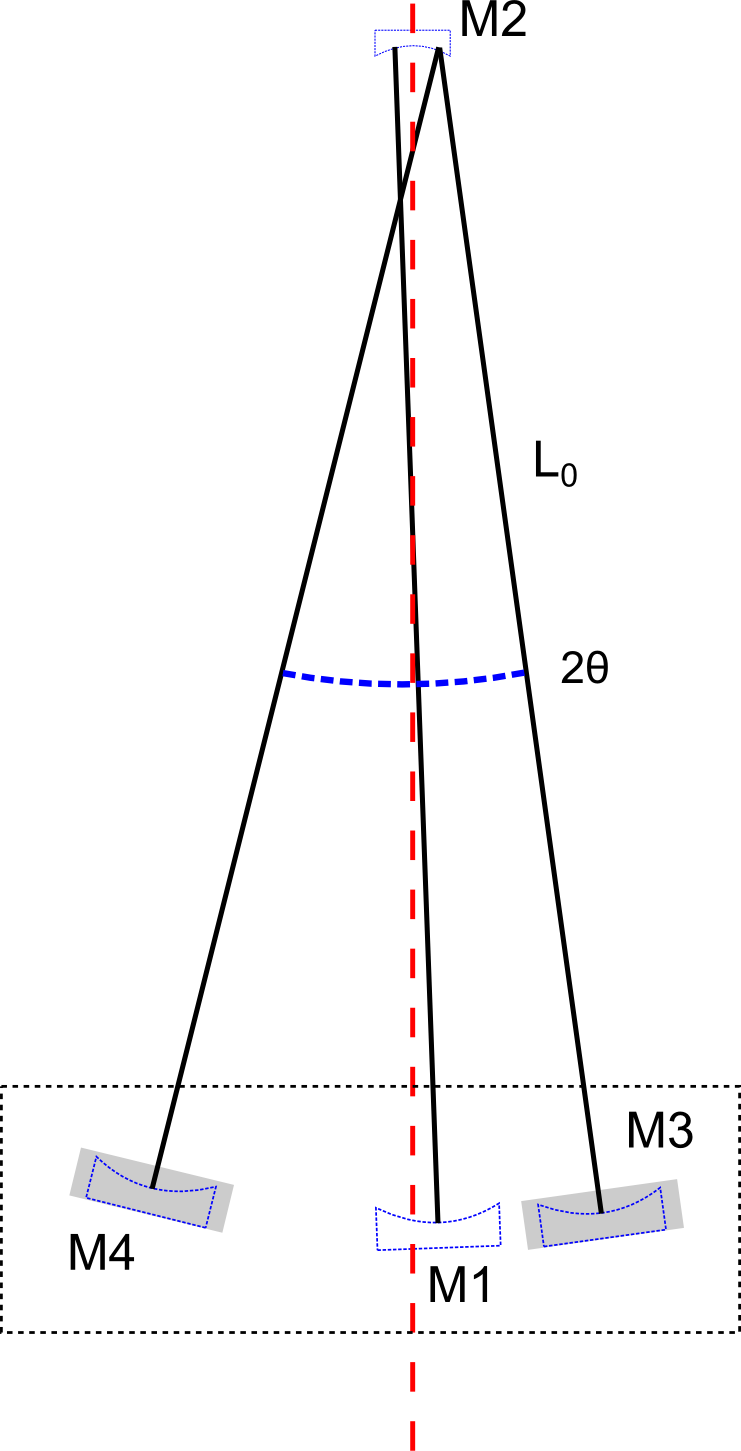
\includegraphics[width=.5\textwidth]{figures/Angular/angularLayout}
\end{center}
\caption[Folded cavity layout]{%
\label{f:angularLayout}
Layout of the angular trap cavity. Light enters through mirrors M1 and M3. The angle $\theta$ of the folded cavity is measured from the normal of M1. 
}
\end{figure}

We can use the same $X$ and $Y$ notation as the original derivation with one small change. $Y=e^{-i\Omega 2\tau}$ is the same, but now $X=(r_1r_2)^2 e^{\frac{-i2\pi L}{\lambda}}$ because the optical path touches M3 and M4 once and M2 twice.

We consider a set of displacements $d_n$, discretely sampled from a continuously oscilating function. This is equivelent to driving the cavity length at angular frequency $\Omega$.  
\begin{eqnarray}
d(t) = x_0e^{i \Omega(t-(2n-1)\tau)}\\
d_1 = x_0e^{i \Omega(t-\tau)}\\
d_n = Y^{2n-2}d_1  
\end{eqnarray}

Following \cite{Perreca14}, we get an equation for the electric field in the cavity, which we must change to reflect that we can only have real values for $d_1$.

\begin{eqnarray}
\label{e:Etot}
E_{tot} = \frac{t_1 E}{1-X}\left[ 1- \frac{4i\pi d_1}{\lambda}\frac{X}{1-Y^2X}\right]\nonumber\\
E_{tot} = \frac{t_1 E}{1-X}\left[ 1- \frac{4i\pi}{\lambda}\left(\frac{ d_1}{1-Y^2X}+\frac{ \overline{d}_1}{1-\overline{Y}^2X}\right)\right]
\end{eqnarray}

Then we get the cavity power:

\begin{eqnarray}
\label{e:P}
P&=&E_{tot}\cdot \overline{E}_{tot}=P_0 t^2\left[ \frac{i 2\pi Y}{\lambda(1-X)(1-\overline{X})}\left(\frac{X}{1-Y^2X}-\frac{\overline{X}}{1-Y^2\overline{X}}\right)\delta L+cc\right]  
%&-&\frac{ikX xY}{(1-\overline{X})(1-X)(1-Y^2 X)} -
%\frac{ikX \bar{x}\overline{Y}}{(1-\overline{X})(1-X)(1-\overline{Y}^2 X)}\nonumber \\
%&+&\frac{ik\overline{X} \bar{x}\overline{Y} } {(1-\overline{X})(1-X)(1-\overline{Y}^2 \overline{X})}+ 
%\frac{ik\overline{X} xY}{(1-\overline{X})(1-X)(1-Y^2 \overline{X})}]  \nonumber \\
%P &=&-P_0t^2 \left[ \frac{ikY}{(1-\overline{X})(1-X)} \left( \frac{X(1+Y^2)}{1-Y^2 X}-\frac{\overline{X}(1+\overline{Y}^2)}{1-Y^2\overline{X}} \right) x + cc \right]?
\end{eqnarray}

We add an extra $Y^{1/2}$ term to get to the other side of the cavity.
It is important to note that the change in cavity length $\delta L$ used here is strictly that: the cavity length. If we want to transpose that into longitudinal change, we need to multiply by a geometric factor (see fig. \ref{f:angularLayout}):

\begin{equation}
\delta L = \frac{2 \delta z}{\mbox{Cos}(\theta)}
\label{e:deltaL}
\end{equation}

There is similarly a geometric correction when calculating the radiation pressure force $F_{rad}$

\begin{eqnarray}
F_{rad} &=& \frac{2r_2^2}{c} P (2 \mbox{Cos}(\theta)) = K_z \delta z\\
&=& \frac{2r_2^2}{c} (2 \mbox{Cos}(\theta)) P_0 t^2\left[ \frac{i 2\pi Y^{3/2}}{\lambda(1-X)(1-\overline{X})}\left(\frac{X}{1-Y^2X}-\frac{\overline{X}}{1-Y^2\overline{X}}\right)\frac{2 \delta z}{\mbox{Cos}(\theta)}+cc\right] 
\label{e:Frad}
\end{eqnarray}

thus 
\begin{equation}
K_z=\frac{4r_2^2}{c} P_0 t^2 \frac{i 4\pi Y^{3/2}}{\lambda(1-X)(1-\overline{X})}\left(\frac{X}{1-Y^2X}-\frac{\overline{X}}{1-Y^2\overline{X}}\right)
\label{eq:Kz}
\end{equation}

With detuning:

\begin{equation}
X \rightarrow X=(r_1r_2)^2 e^{-i2\delta\tau}
\label{e:Xdet}
\end{equation}

Here $\delta = \omega_0-\omega_{res}$, the angular frequency detuning from the cavity resonance, $\omega_{res} = 2\pi n c/L$, and $\omega_0$ is the frequency of the laser.

\begin{eqnarray}
K_{OS}=&-P_0 t^2 r_2^2 \frac{16i\pi e^{-\frac{3}{2}i\Omega\tau}}{\lambda c(1-(r_1r_2)^2e^{i2\delta\tau})(1-(r_1r_2)^2e^{-i2\delta\tau})}\times\nonumber\\
 & \left( \frac{(r_1r_2)^2e^{-i\delta \tau}}{1-(r_1r_2)^2e^{-2i\Omega\tau} e^{-i2\delta\tau}}
 -\frac{(r_1r_2)^2e^{i2\delta\tau}}{1-(r_1r_2)^2e^{-2i\Omega\tau}e^{i2\delta\tau}} \right) 
\end{eqnarray}

Considering the finesse for the folded cavity to be $F = \pi\frac{FSR}{\gamma} \approx \frac{\pi}{1-(r_1r_2)^2} $

keep in mind that we have half the FSR of a non-folded cavity and half the finesse, so $\gamma$ is the same here as it is for the longitudinal trap.

\begin{eqnarray}
\label{eq:KOSfold}
K_{OS} & {\approx} & P_0 t_1^2 \frac{32k}{c(1-(r_1r_2)^2)^3}\frac{ \frac{\delta}{\gamma}}{(1+\frac{\delta^2}{\gamma^2})} 
\frac{1}{1+\frac{\delta^2}{\gamma^2}-\frac{\Omega^2}{\gamma^2}+i2\frac{\Omega}{\gamma} }
\end{eqnarray}

This is important because it means that a folded cavity angular spring will behave differently. Namely, the folded cavity spring constant is four times larger in magnitude than a similar straight cavity.

\subsection{angular issues}
worried about the change in beam shape
not an issue (but did lock on TEM01)
\begin{figure}[htp]%
\begin{center}
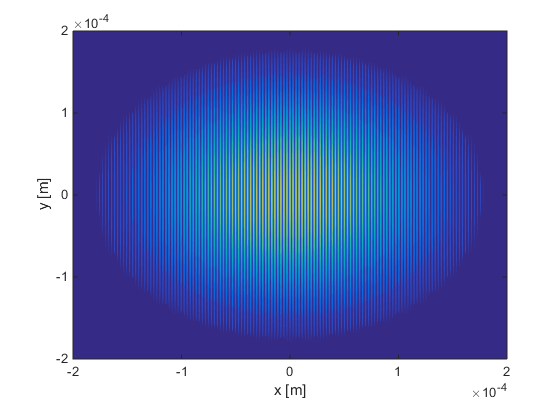
\includegraphics[width=.8\textwidth]{figures/Angular/11deginterference}%lab\lab2014\OpticalLayout\20140903_angular_options
\caption[Folded cavity interference pattern]{Simulated folded cavity interference pattern on the surface of M2. This corresponds to the power deposited into the mirror and thus the amplitude of the photothermal effect. Using this and the diffusion length as a function of frequency, we showed that there would be no significant amplification of the photothermal effect due to this distribution of absorbed power.}%
\end{center}
\label{fig:foldedinterference}%
\end{figure}

shape of power distribution on end mirror.

%\Chapter{Application}
%\label{ch:application}
%\section{Motivation}

Angular control in LIGO is an important contribution to the noise budget at the frequencies of highest sensitivity \cite{T0900511}. 

There are four different angular modes for the two Fabry-Perot arms in the LIGO interferometer, shown in figure \ref{fig:sidlessiggmodes}. 
The two hard modes are stable as the power increases, which means that the radiation pressure will push the mirrors back to an equilibrium position.
The two soft modes are unstable as the power increases, pushing the mirrors away from equilibrium. 
Despite being stable, the hard modes still exhibit a resonant behavior that will need to be damped.

\begin{figure}[htp]%
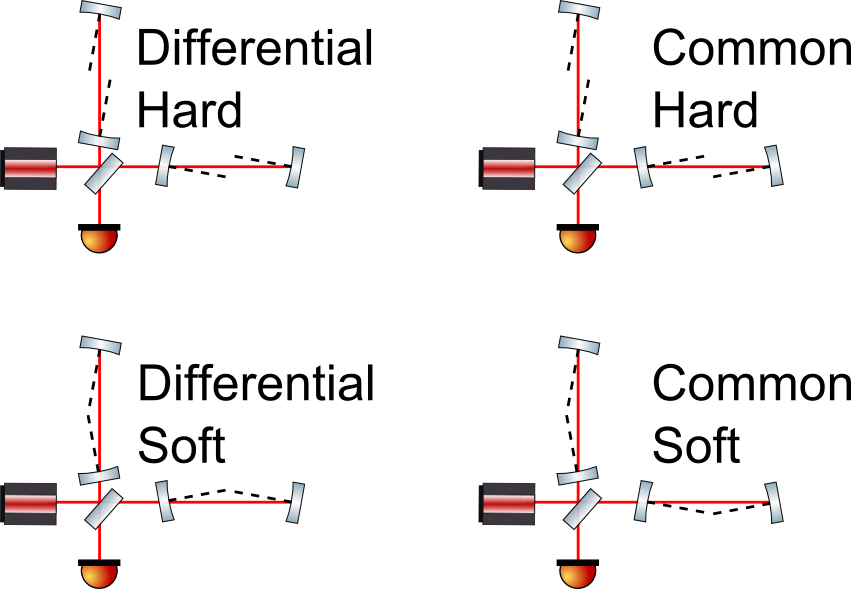
\includegraphics[width=.8\textwidth]{figures/application/SidlesSigg}%
\caption[Sidles-Sigg Modes]{The four Sidles-sigg modes of the Fabry-Perot cavities in LIGO. The two hard modes are stable and the two soft modes are unstable. All of modes must be damped with control loops.}%
\label{fig:sidlessiggmodes}%
\end{figure}

Angular noise can couple in to differential arm length (DARM) though the interaction between beam spot motion (BSM) and angular motion ($\theta$) on mirrors. This happens in two ways: both a static offset in the BSM with mirror angular noise and a static angular offset with BSM noise can create DARM noise. 

\begin{equation}
\hat{\Delta L}(f) = \hat{d}_{spot}(f)*\hat{\theta}_{Mirror}(f) \approx \hat{d}_{spot}(f)*\theta_{Mirror}^{RMS}(f) + d_{spot}^{RMS}(f)*\hat{\theta}_{Mirror}(f)
\label{eq:darmcouple}
\end{equation}

Barsotti and Evans showed that in Science Mode, angular noise from Common Soft and Differential Soft (the two modes of the arms that are unstable at high power) contribute the most to DARM noise. They also showed that in the final design of aLIGO, the soft mode is unstable with frequencies of -.17 and -.21 Hz for pitch and yaw, respectively. The control systems currently used for angular control must be used to damp the unstable modes and the resonances of the stable modes, which leads to injected sensing noise. For an optical angular control system to be useful, it must provide damping in that frequency range to stabilize the modes.

Using angular trapping methods, we can reduce the sensing noise injection by damping the angular motion $\hat{\theta}_{Mirror}(f)$.

\section{Applying angular control}

For our discussion, we will disregard the distinction between common and differential modes of the interferometer.

%I have considered two possible options that could (with some effort) be implemented in a LIGO-style interferometer.
%
%\subsection{Local damping}
%
%Damping relative to something very heavy in the end station. This is analogous to (and much harder than) just increasing the mass of the test mass.
%
%BSC4 layout: D0901154
%
%Pros:
%
%\begin{itemize}
	%\item Can keep the same ETM/ITM suspensions
	%\item Modular: easy to modify and/or disable
	%\item Easier to build, align and lock
	%\item Affects Soft and Hard modes equally.
%\end{itemize}
%
%Cons:
%\begin{itemize}
  %\item	Different parameters for ETM and ITM
	%\item Folded Cavities
	%\item worry about ISI weight limit
%\end{itemize}
%
%
%
%\begin{figure}[htp]%
%\begin{center}
%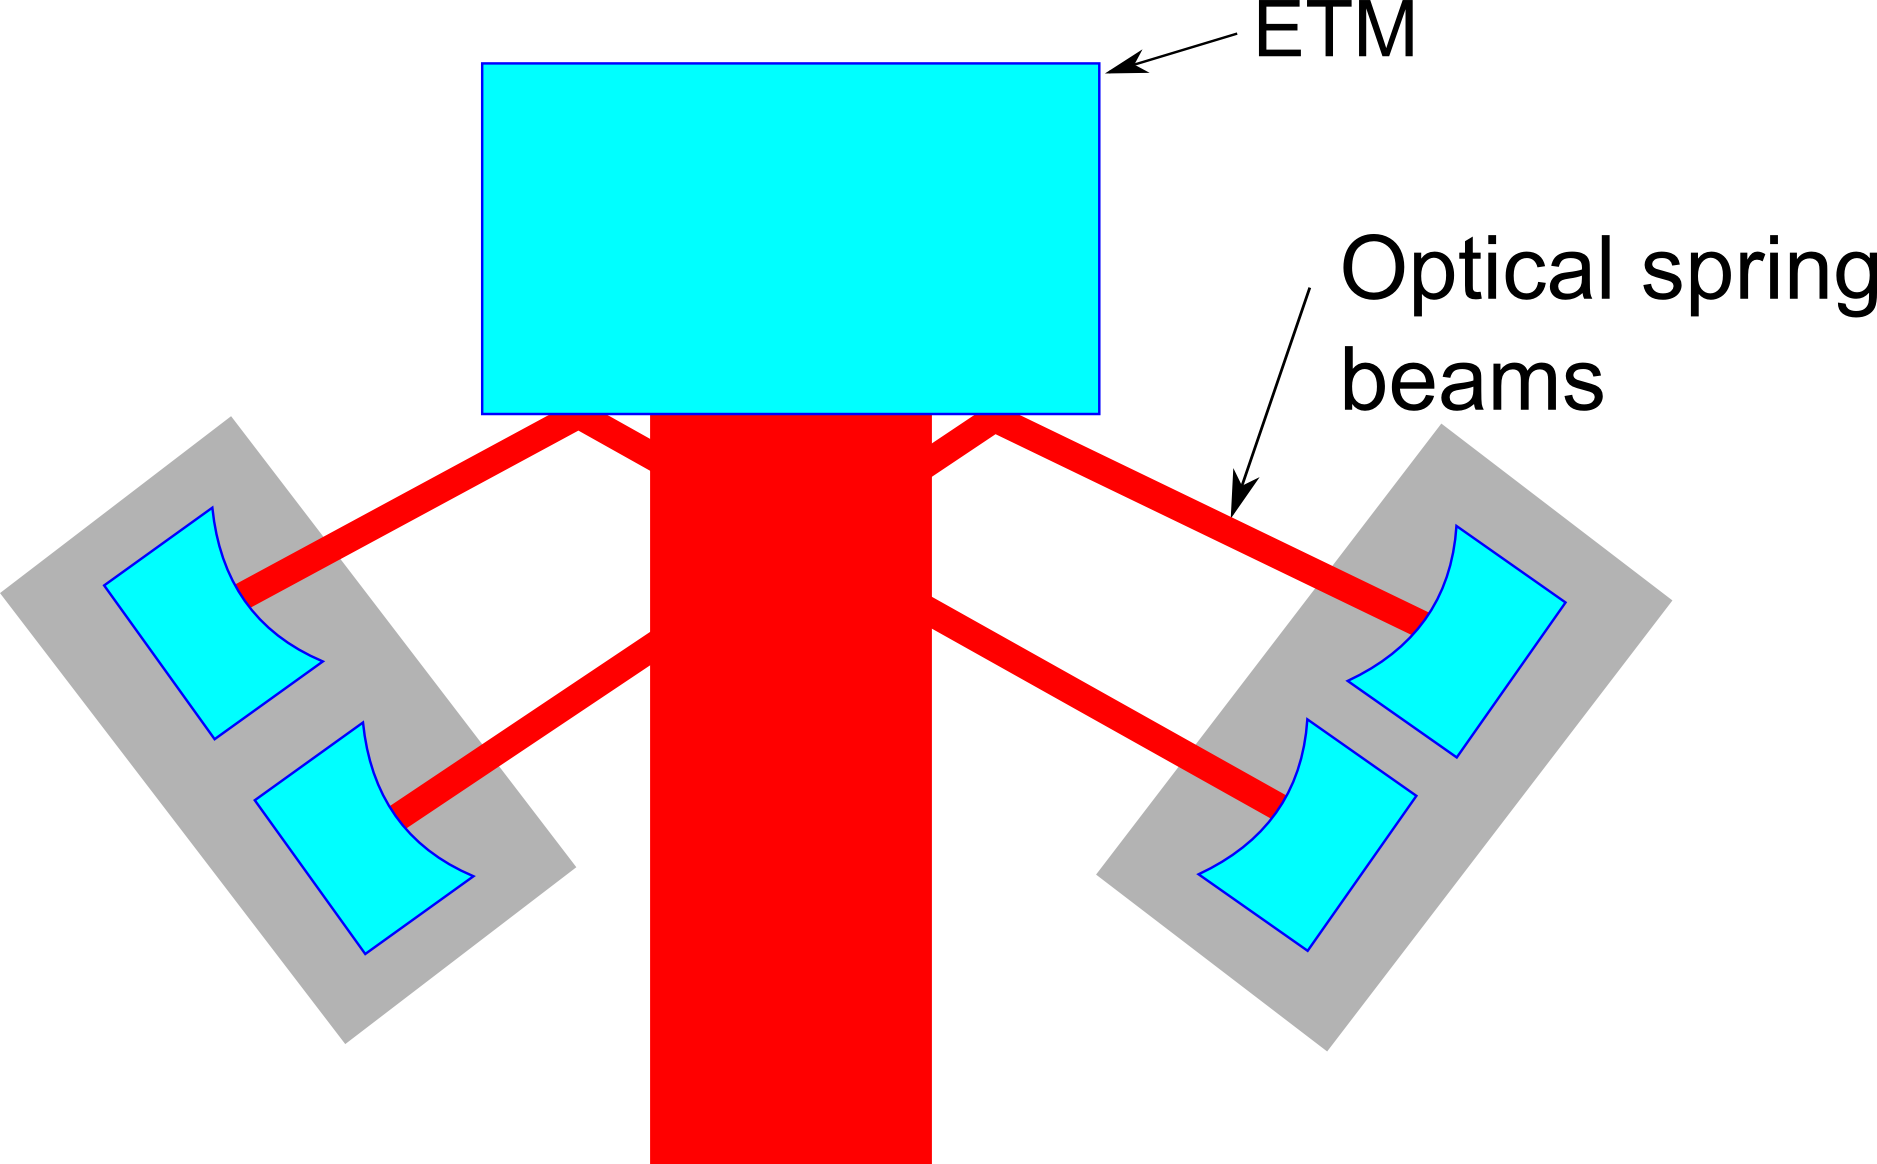
\includegraphics[width=.8\textwidth]{figures/application/shortTrapDiagram}%
%\caption[Local angular control]{Diagram of a local angular control scheme. This relies on the small mirrors being mounted in something heavier than the test mass.}%
%\label{fig:shorttrapdiagram}%
%\end{center}
%\end{figure}
%
%
%\begin{table}[htp]
%\centering
%\begin{tabular}{ l | l | }
%\bf{Parameter}& \bf{Metric}  \\ \hline
%Cavity length, $L$ & 2 m \\ \hline
%ETM power transmission, $T2$ & 5 ppm \\ \hline
%ETM $r2$ &0.9999975 \\ \hline
%ETM Diameter $D$ & 34 cm \\ \hline
%ETM Thickness $t$ & 20 cm \\ \hline
%Side diameter $D_s$ & 48 cm \\ \hline
%Side thickness $t_s$ & 30 cm \\ \hline
%Side ROC & 1.5 m \\ \hline
%Cavity $FSR$ & 75 MHz \\ \hline
%
%\end{tabular}
%\caption[Local angular design]{Characteristics of proposed local angular design}
%\label{tab:localproposal}
%\end{table}
%
%\begin{table}[htp]
%\centering
%\begin{tabular}{ l | l | }
%\bf{Parameter}& \bf{Metric}  \\ \hline
%Carrier Power $P_c$ & 10 W \\ \hline
%Subcarrier Power $P_s$ & 2 W \\ \hline
%Carrier Detuning $df_c$ & 9000 Hz \\ \hline
%Subcarrier Detuning $df_s$ & -2500 Hz \\ \hline
%OS Angle $\theta$ & 45 deg \\ \hline
%\end{tabular}
%\caption[Local angular optical springs]{Characteristics of proposed local angular optical spring}
%\label{tab:localos}
%\end{table}
%
%In this design, we use radiation pressure to couple e.g. the ETM (about 40 kg) to two much larger masses (about 400 kg each) made out of stainless steel. In this fashion, we can damp the angular motion of the test mass relative to the hopefully much more stable masses on the side. 
%
%With the control beams at \~ 45 degrees to the optical axis, we expect that the coating will be significantly lower reflectivity. Er-glass lasers at 1540 nm 
%
%\subsection{4 km damping}
%
%\begin{figure}[htp]%
%\begin{center}
%\includegraphics[width=.8\textwidth]{figures/application/longTrapDiagram}%
%\caption[4 km angular control]{Diagram of a 4km angular control scheme. This relies on control mirrors attached to the side of the test mass.}%
%\label{fig:longtrapdiagram}%
%\end{center}
%\end{figure}
%
%Damping ETM relative to ITM. This will have significant changes because the masses of the ETM and ITM are currently the same. The angular trap we have damps the motion of one mirror by pushing on the other. In a system with equal masses, this just couples the mirrors, it doesn't damp. 
%
%Pros:
%
%\begin{itemize}
	%\item Straight cavities
	%\item Lower vacuum chamber volume
	%\item Damp only Soft mode
%\end{itemize}
%
%Cons:
%\begin{itemize}
	%\item Does not see Hard mode motion of cavity
	%\item Modify test masses and probably suspensions
	%\item Hard/risky to adjust
%\end{itemize}
%
%
%\begin{table}[htp]
%\centering
%\begin{tabular}{ l | l | }
%\bf{Parameter}& \bf{Metric}  \\ \hline
%Cavity length, $L$ & 3994.5 m \\ \hline
%ITM power transmission, $T1$ & 1.4\% \\ \hline %T0900043

%ETM power transmission, $T2$ & 5 ppm \\ \hline
%ITM $r1$ & 0.99298 \\ \hline
%ETM $r2$ &0.9999975 \\ \hline
%Cavity $FSR$ & 37.52 kHz \\ \hline
%\end{tabular}
%\caption{Characteristics of proposed long angular design}
%\label{tab:longproposal}
%\end{table}
%
\subsection{Single spring 4km damping}

If we assume that the length will be stabilized with the main beam of the interferometer, we only really need to control the angular motion. We will consider only the yaw of the mirrors for this exploration, but there should not be any obstacles to applying the method to both pitch and yaw. 

It seems like we could do this with a single folded cavity (see fig \ref{fig:longtrapfoldeddiagram}). In this configuration, ETMs and ITMs would have `Buddy' mirrors attached to the sides to create an angular optical spring cavity.

This has several benefits that look quite appealing. The yaw of the ETM is damped relative to the ITM. If implemented ideally, the radiation pressure will be independent of small angular motions of the ETM. This particular configuration (see table \ref{tab:foldedos} has a UGF of about 8 Hz, so it should also damp the hard mode (Barsotti and Evans give a hard mode frequency of 3.05 Hz). This would also, as a byproduct, give a very sensitive readout of the yaw of the ETM via the PDH error signal.

There are several concerns that would need to be addressed. This configuration could actively couple angular noise in the ITM into length noise at the ETM. It would also require massive engineering changes to manufacture and align a monolithic test mass with Buddy mirrors bonded onto the sides. These mirrors would also need to be very carefully manufactured and attached, because the cavity could not be realigned once assembled.  

The design has to be careful of losses due to long-storage-time optical cavities\cite{Isogai13}, but the finesse is low enough in this configuration ($F=7850$) to avoid a significant impact from the effects. The design also has the potential to introduce increased thermal noise to the length degree of freedom, due to the added buddy mirrors. We have neglected the thermal noise effects in this analysis, but it should be addressed.


\begin{table}[htp]
\centering
\begin{tabular}{ l | l | }
\bf{Parameter}& \bf{Metric}  \\ \hline
Cavity round-trip length, $4L$ & 16 Km \\ \hline
Buddy Mirror power transmission, T1,T2 & 200 ppm \\ \hline
Buddy Mirror power absorption, T1, T2 & 2 ppm \\ \hline
Buddy Diameter $D$ & 15 cm \\ \hline
Buddy Thickness $t$ & 10 cm \\ \hline
Buddy ROC & 3.5 km \\ \hline
Cavity $FSR$ & 18.7  kHz \\ \hline
Cavity Finesse & 7850 \\ \hline

\end{tabular}
\caption[Folded angular design]{Characteristics of proposed angular design. The transmissivity and absorption values are easily achievable with current dielectric coatings.}
\label{tab:foldedproposal}
\end{table}

\begin{table}[htp]
\centering
\begin{tabular}{ l | l | }
\bf{Parameter}& \bf{Metric}  \\ \hline
Carrier input power $P_c$ & 6 W \\ \hline
Subcarrier input power $P_s$ & .15 W \\ \hline
Carrier Detuning $df_c$ & 19 Hz \\ \hline
Subcarrier Detuning $df_s$ & -5 Hz \\ \hline
OS Angle $\theta$ & 62.5 $\mu rad$ \\ \hline
OLG UGF & 7.9 Hz \\ \hline
Phase at UGF & -169.3 deg \\ \hline
\end{tabular}
\caption[Folded angular optical springs]{Characteristics of proposed angular optical spring. The relatively low power (about 6 watts) is easily achievable. The detunings will require careful design because they are very small.}
\label{tab:foldedos}
\end{table}

Table \ref{tab:foldedos} lists the parameters for a possible optical spring design. If we lock the laser to the frequency of the main cavity laser, we can take advantage of the fantastic frequency stabilization of a 4 km cavity, and also remove the common mode length noise of associated with relative frequency fluctuations. The very small frequency detunings would still present a significant challenge to implement and maintain.

\begin{figure}[htp]%
\begin{center}
\includegraphics[width=.6\textwidth]{figures/application/longFoldedDiagram}%
\caption[4 km angular control]{Diagram of a folded cavity 4km angular control scheme. This configuration relies on `Buddy' mirrors attached to the side of the test masses.}%
\label{fig:longtrapfoldeddiagram}%
\end{center}
\end{figure}

\begin{figure}[htp]%
\begin{center}
\includegraphics[width=\textwidth]{figures/application/OLG}%
\caption[4 km angular open loop gain]{Open loop gain ($OLG$) of the angular control scheme and optical springs. The optical springs shown are the carrier and subcarrier optical spring constants ($KOS_C$ and $KOS_S$) and the total optical spring ($KOS_T$).}%
\label{fig:longtrapfoldedOLG}%
\end{center}
\end{figure}

\begin{figure}[htp]%
\begin{center}
\includegraphics[width=\textwidth]{figures/application/SAF}%
\caption[4 km angular closed loop gain]{The actuation function ($ACF$) and spring actuation function ($SAF = CLG\times ACF$) of the proposed angular control scheme. The actuation function includes the yaw pendulum behavior ($1/f^2$) of the mass and the yaw resonant frequency (chosen to be 0.5 Hz) of the ETM. }%
\label{fig:longtrapfoldedSAF}%
\end{center}
\end{figure}



%\section{noise benefits}
%
%The cool thing about this method is that it can work independently and in tandem with existing control systems. 

%\section{path to angular damping with optical springs in aLIGO}
%
%I think we might want to get rid of this section.
%\Chapter{Conclusion}
%\label{ch:conclusion}
%\section{Summary}

aLIGO has begun taking data and will achieve design sensitivity over the next few years. At that point, the next generation of upgrades and improvements must be nearly ready to implement. One possible such upgrade would be to damp the unwanted angular motion in the test masses using radiation pressure feedback. This has the potential benefits of reducing the angular noise of the system and thus also reducing the amount of noise that couples from angular motion into cavity length.  
 
We have explored the implementation and uses of radiation pressure feedback, optical springs, to control the motion of a mirror. 
We demonstrated in several ways the underlying principles and behavior of optical springs, in both straight and folded cavities.
We discussed the mechanical design of the experiment, with the addition of blade springs to reduce the influence of seismic noise on the experiment.
We reviewed the feedback and controls in use for the optical traps. 
We measured and modeled the causes and effects of the photothermal effect in an optical spring system.
We explored one- and two-degree-of-freedom traps, and, while we could not get the angular trap stably locked for more than two seconds, we have laid out the path to do so.
We designed and modeled a full-scale implementation of angular optical springs to damp the Sidles-Sigg instability in the aLIGO configuration.

These developments should lay a strong groundwork for continued research into the applications and uses of radiation pressure feedback in aLIGO and beyond.

\section{Future work}

There are several things left unfinished that will hopefully deliver interesting results:

\begin{enumerate}
	\item Improving the stability  of the SU angular optical trap experiment and damping the 66 Hz resonance that seems to be preventing extended locks.
	There are a number of possibilities to increase the bandwidth and damp the motion outlined in Section \ref{sec:bandwidth}.
	\item Exploring the possibility of a a single stable optical spring with a specialized optical coating.
	We expect that dielectric coating manufacturers could do a custom run with a very thick first layer to create a ``self-locking'' cavity. The mirror could be mounted using the same cold weld method described in Section \ref{sec:endMirror}, then tested with the single-mirror input coupler from Chapter \ref{ch:photothermal}. 
	\item Designing and demonstrating a large scale angular trap in aLIGO.
	A detailed noise budget needs to be drafted using a modified version of GWINC or a similar tool to insure that we would not be introducing too much thermal noise.
	After that, a prototype of the design would need to be built at e.g. the Caltech 40 m interferometer to develop control systems and test predictions.
\end{enumerate}

%For each bullet, add at lease one more sentence that discusses how you would go about these items.
%What is the first thing to be done? What hardware needs to be purchased, changed? Etc.


%% $Id$
%
%Although the upper limit that we have placed on the rate of binary black hole
%MACHO inspirals in the galaxy is lower than the upper bound of the predicted
%rates, the LIGO interferometers were not at design sensitivity when the S2
%data was taken. At present, the sensitivities of the instruments are
%significantly better than during S2, as can be seen from
%figure~\ref{f:s3strain}, and progress on reducing noise in the interferometers
%continues apace.  The increase in detector sensitivity makes a larger volume
%of the Universe accessible to searches for binary inspirals. In addition to
%this, the amount of data is also increasing as the interferometers become more
%stable.
%
%These improvements in the instruments will increase the chance of detecting
%gravitational waves from binary inspirals. If the rates of binary black hole
%MACHO coalescence are truly as high as predicted, then initial LIGO would
%stand an excellent chance of detecting an inspiral. The first detection of
%gravitational waves will be a major scientific breakthrough and will yield and
%enormous amount of scientific information, particularly if the detection came
%from a binary black hole MACHO. The length of binary black hole MACHO
%inspirals in the sensitive band of the interferometer will allow extremely
%accurate parameter estimation as well as tests of post-Newtonian theory. For
%systems with total mass greater than $\sim 0.64\,\mathrm{M}_\odot$ LIGO will
%be sensitive to the coalescence of the binary and will be able to study the
%strong gravitational field effects when two binary black holes merge. When
%this is coupled with the accurate parameter estimation available from the
%earlier part of the waveform, the inspiral of a binary black hole MACHO could
%be an excellent laboratory for General Relativity.  A detection would also
%impact the studies of halo dark matter and early universe physics, providing a
%MACHO component to the halo and suggesting that primordial black holes do
%indeed form in the universe.
%
%In the absence of detection, the improvements in detector sensitivity will
%dramatically improve the upper limits placed on the rate of binary black hole
%MACHO inspirals. Once these rates are below the predicted rates, we may begin
%to use observations from gravitational wave interferometers to constrain the
%fraction of galactic halos in the form of primordial black hole MACHOs. While
%this may not be as significant as a detection, it will still be of interest to
%the astrophysical community.
%
%\newpage 
%
%\begin{figure}[p]
%\vspace{5pt}
%\begin{center}
%\includegraphics[width=\textwidth]{figures/conclusion/s3strain}
%\end{center}
%\caption[Comparison of Best LIGO Interferometer Sensitivity]{%
%\label{f:s3strain}
%Comparison of the best sensitivities of the LIGO interferometers between
%science runs. The solid curve shows the design sensitivity for the $4$~km
%interferometers: the LHO $4$~km is only a factor of $\sim 2$ away from design
%at $100$~Hz during S3.
%}
%\end{figure}
%


%\appendix
%\Chapter{Beam Separation}
%\label{ap:beamseparation}
%%\documentclass[12pt]{article}
%\usepackage{fullpage,graphicx}
%\title{Beam seperation}
%\author{David Kelley}
%\begin{document}
%\maketitle

\section{Definitions}
\begin{itemize}
\item $P_m$ Input power of the main beam 
\item $P_s$ Input power of the side beam
\item $f_m$ Main cavity finesse
\item $f_s$ Side cavity finesse
\item $R_c$ Radius of curvature of payload mirror (5 cm)
\item $\theta_m$ Main beam angle from optical axis.  Origin is at center of curvature.
\item $\theta_s$ Side beam angle from optical axis.  Origin is at center of curvature.
\item $c$ Speed of light
\item $R$ Payload mirror radius
\item $h$ Payload mirror thickness
\item $m$ Payload mirror mass
\item $I = \frac{m}{12}(3R^2+h^2)$ Payload mirror moment of inertia
\item $G = \frac{P_mf_m}{P_sf_s}$ Handy constant
\item $d = \theta_mR_c - \theta_sR_c$ Beam spot seperation
\end{itemize}


\newpage
\section{Balancing torques}
We want the mirror to be stationary, so the net torque on the mirror should be zero.

Force on payload mirror due to radiation pressure of the two beams:

$$ F_m = \frac{2P_mf_m}{c} \hspace{20 pt} F_s = \frac{2P_sf_s}{c}$$

$$\tau = F_m\theta_mR_c+F_s\theta_sR_c = 0$$

substituting in $d$,

$$\theta_m = \frac{d}{R_c(1+G)}$$

\section{Eliminating beam coupling}

We propose that there is a spot somewhere on the surface of the payload mirror where the sum of torque and force due to one beam makes the net force zero.  We place one beam spot at $r_1$.  We'd like to put the other beam in the null spot $r_2$ so that there is no force coupling between the two.  

$$Fs=\frac{2P_sf_s}{c} = m\omega^2x \hspace{20pt} x = \frac{F_s}{m\omega^2}$$ 
$$\tau_s = F_sr_1=I\omega^2\phi \hspace{20pt} \phi = \frac{F_s r_1}{I\omega^2}$$

Let's find a point these effects cancel:

$$r_2\phi-x=0 \hspace{20 pt} r_2=\frac{x}{\phi}=\frac{I}{mr_1}$$

It should be noted that the previously used $d$ can also be expressed as $d =r_2-r_1$.

$$r_2 = \theta_2R_c = \theta_mR_c$$

$$r_2 = \frac{d}{1+G}$$

$$\frac{I}{m} = \frac{(r_2-r_1)r_1}{1+G} = \frac{\left(\frac{I}{mr_1}+r_1\right)r_1}{1+G}$$

$$r_1 = \sqrt{\frac{I}{mG}} \hspace{20pt} r_2 = \sqrt{\frac{IG}{m}}$$

These radii are the ideal horizontal distances from the payload mirror optical axis to the beam spots.
%A MATLAB script that computes this seperation is included in this directory, named cavityAngles.m. 



%\end{document}

\clearpage
\bibliographystyle{unsrt}
\bibliography{references}

\addcontentsline{toc}{chapter}{\numberline {Bibliography}}

\clearpage
\birthplacedate{Poughkeepsie, New York \>\>December 3, 1987}
\collegewherewhen{%
\>Massachusetts Institute of Technology \>\>2006--2010, \>B.S.\\
\>\su	\>\>2010--2015, \>Ph.D.}

\newpage
\null\vskip1in%
\begin{center}
{\Large\bf Curriculum Vitae}
\end{center}
\vskip 2em
\begin{tabbing}
\tabset
Title of Dissertation\\
\>Angular trapping of a mirror using radiation pressure
\end{tabbing}
\vskip 1em

\begin{startvita}
\end{startvita}

\renewenvironment{thebibliography}[1]%
  {\begin{list}{\labelenumi\hss}%
     {\usecounter{enumi}\setlength{\labelwidth}{3em}%
      \setlength{\leftmargin}{5em}}}%
  {\end{list}}
\renewcommand{\bibitem}[1]{\item\label{#1}\relax}%
\renewcommand{\theenumi}{\arabic{enumi}}%
\begin{publications}
\putbib[papers]
\end{publications}

\begin{honorarysocieties}
2010 \> Fellowship??\\
\end{honorarysocieties}

\finishvita
\end{document}
